% AUTO-GENERATED by writeup/make_rehaul_channels.py -- do not edit; re-run the script.
\ifdefined\rhchNBars\else% AUTO-GENERATED by writeup/make_rehaul_channels.py -- do not edit; re-run the script.
% \rhch... macros: the two channels of the pooled gain (results/channels_2026-10-26/RULE.txt items 1-3):
% FOMC statement days (EVENT) and ordinary days, Table 1's scored bars, the FOMC-patched design of record;
% DM (HLN) on daily average loss, lag 8.  Names in the generator's docstring.
% \rhchX... = ADDITIONAL, NOT PRE-REGISTERED (coordinator, 2026-10-26, after the first scoring): the full set
% against HAR + the futures' realized moments (FullVsRm) and HAR + realized moments against HAR (RmVsHar).
\providecommand{\rhPending}{\textit{pending}}
\providecommand{\rhchNBars}{}\renewcommand{\rhchNBars}{33{,}527}  % scored bars (Table 1)
\providecommand{\rhchNDays}{}\renewcommand{\rhchNDays}{2{,}579}  % scored days
\providecommand{\rhchNEventDays}{}\renewcommand{\rhchNEventDays}{81}  % EVENT days: scheduled FOMC statement days of the span
\providecommand{\rhchNOrdDays}{}\renewcommand{\rhchNOrdDays}{2{,}498}  % ORDINARY days
\providecommand{\rhchNEventBars}{}\renewcommand{\rhchNEventBars}{1{,}053}  % bars on EVENT days
\providecommand{\rhchEventBarPct}{}\renewcommand{\rhchEventBarPct}{3.1}  % EVENT-day bars, % of the scored bars
\providecommand{\rhchHacLag}{}\renewcommand{\rhchHacLag}{8}  % Newey-West lag of every DM test
\providecommand{\rhchAgreePp}{}\renewcommand{\rhchAgreePp}{2}  % item 1: the corrections agree within this many percentage points
\providecommand{\rhchLadderDesign}{}\renewcommand{\rhchLadderDesign}{patched}  % design of the ladder
\providecommand{\rhchRidgeTabOnePct}{}\renewcommand{\rhchRidgeTabOnePct}{$-$6.0}  % ridge: full vs HAR, every bar (Table 1): % QLIKE change
\providecommand{\rhchRidgeTabOneDm}{}\renewcommand{\rhchRidgeTabOneDm}{$-$6.28}  % ridge: full vs HAR, every bar (Table 1): DM
\providecommand{\rhchRidgeTabOneP}{}\renewcommand{\rhchRidgeTabOneP}{\ensuremath{<}0.001}  % ridge: full vs HAR, every bar (Table 1): DM p
\providecommand{\rhchRidgeTabOneMsePct}{}\renewcommand{\rhchRidgeTabOneMsePct}{100.6}  % ridge: full vs HAR, every bar (Table 1): % MSE change
\providecommand{\rhchRidgeTabOneMseP}{}\renewcommand{\rhchRidgeTabOneMseP}{0.261}  % ridge: full vs HAR, every bar (Table 1): DM p on MSE
\providecommand{\rhchRidgeCorrAPct}{}\renewcommand{\rhchRidgeCorrAPct}{$-$3.0}  % ridge: full vs HAR+FOMC, every bar: % QLIKE change
\providecommand{\rhchRidgeCorrADm}{}\renewcommand{\rhchRidgeCorrADm}{$-$3.64}  % ridge: full vs HAR+FOMC, every bar: DM
\providecommand{\rhchRidgeCorrAP}{}\renewcommand{\rhchRidgeCorrAP}{\ensuremath{<}0.001}  % ridge: full vs HAR+FOMC, every bar: DM p
\providecommand{\rhchRidgeCorrAMsePct}{}\renewcommand{\rhchRidgeCorrAMsePct}{100.8}  % ridge: full vs HAR+FOMC, every bar: % MSE change
\providecommand{\rhchRidgeCorrAMseP}{}\renewcommand{\rhchRidgeCorrAMseP}{0.258}  % ridge: full vs HAR+FOMC, every bar: DM p on MSE
\providecommand{\rhchRidgeCorrBPct}{}\renewcommand{\rhchRidgeCorrBPct}{$-$3.2}  % ridge: full without FOMC vs HAR, every bar: % QLIKE change
\providecommand{\rhchRidgeCorrBDm}{}\renewcommand{\rhchRidgeCorrBDm}{$-$3.74}  % ridge: full without FOMC vs HAR, every bar: DM
\providecommand{\rhchRidgeCorrBP}{}\renewcommand{\rhchRidgeCorrBP}{\ensuremath{<}0.001}  % ridge: full without FOMC vs HAR, every bar: DM p
\providecommand{\rhchRidgeCorrBMsePct}{}\renewcommand{\rhchRidgeCorrBMsePct}{102.3}  % ridge: full without FOMC vs HAR, every bar: % MSE change
\providecommand{\rhchRidgeCorrBMseP}{}\renewcommand{\rhchRidgeCorrBMseP}{0.258}  % ridge: full without FOMC vs HAR, every bar: DM p on MSE
\providecommand{\rhchRidgeCorrCPct}{}\renewcommand{\rhchRidgeCorrCPct}{$-$3.2}  % ridge: full vs HAR, ORDINARY days: % QLIKE change
\providecommand{\rhchRidgeCorrCDm}{}\renewcommand{\rhchRidgeCorrCDm}{$-$3.51}  % ridge: full vs HAR, ORDINARY days: DM
\providecommand{\rhchRidgeCorrCP}{}\renewcommand{\rhchRidgeCorrCP}{\ensuremath{<}0.001}  % ridge: full vs HAR, ORDINARY days: DM p
\providecommand{\rhchRidgeCorrCMsePct}{}\renewcommand{\rhchRidgeCorrCMsePct}{110.2}  % ridge: full vs HAR, ORDINARY days: % MSE change
\providecommand{\rhchRidgeCorrCMseP}{}\renewcommand{\rhchRidgeCorrCMseP}{0.258}  % ridge: full vs HAR, ORDINARY days: DM p on MSE
\providecommand{\rhchRidgeCorrAgree}{}\renewcommand{\rhchRidgeCorrAgree}{agree}  % ridge: the three corrections within 2.0 pp?
\providecommand{\rhchRidgeCorrSpread}{}\renewcommand{\rhchRidgeCorrSpread}{0.2}  % ridge: max - min of the three (pp)
\providecommand{\rhchLassoTabOnePct}{}\renewcommand{\rhchLassoTabOnePct}{$-$9.0}  % lasso: full vs HAR, every bar (Table 1): % QLIKE change
\providecommand{\rhchLassoTabOneDm}{}\renewcommand{\rhchLassoTabOneDm}{$-$6.34}  % lasso: full vs HAR, every bar (Table 1): DM
\providecommand{\rhchLassoTabOneP}{}\renewcommand{\rhchLassoTabOneP}{\ensuremath{<}0.001}  % lasso: full vs HAR, every bar (Table 1): DM p
\providecommand{\rhchLassoTabOneMsePct}{}\renewcommand{\rhchLassoTabOneMsePct}{114.7}  % lasso: full vs HAR, every bar (Table 1): % MSE change
\providecommand{\rhchLassoTabOneMseP}{}\renewcommand{\rhchLassoTabOneMseP}{0.247}  % lasso: full vs HAR, every bar (Table 1): DM p on MSE
\providecommand{\rhchLassoCorrAPct}{}\renewcommand{\rhchLassoCorrAPct}{$-$3.4}  % lasso: full vs HAR+FOMC, every bar: % QLIKE change
\providecommand{\rhchLassoCorrADm}{}\renewcommand{\rhchLassoCorrADm}{$-$3.20}  % lasso: full vs HAR+FOMC, every bar: DM
\providecommand{\rhchLassoCorrAP}{}\renewcommand{\rhchLassoCorrAP}{0.001}  % lasso: full vs HAR+FOMC, every bar: DM p
\providecommand{\rhchLassoCorrAMsePct}{}\renewcommand{\rhchLassoCorrAMsePct}{114.4}  % lasso: full vs HAR+FOMC, every bar: % MSE change
\providecommand{\rhchLassoCorrAMseP}{}\renewcommand{\rhchLassoCorrAMseP}{0.243}  % lasso: full vs HAR+FOMC, every bar: DM p on MSE
\providecommand{\rhchLassoCorrBPct}{}\renewcommand{\rhchLassoCorrBPct}{$-$2.8}  % lasso: full without FOMC vs HAR, every bar: % QLIKE change
\providecommand{\rhchLassoCorrBDm}{}\renewcommand{\rhchLassoCorrBDm}{$-$2.75}  % lasso: full without FOMC vs HAR, every bar: DM
\providecommand{\rhchLassoCorrBP}{}\renewcommand{\rhchLassoCorrBP}{0.006}  % lasso: full without FOMC vs HAR, every bar: DM p
\providecommand{\rhchLassoCorrBMsePct}{}\renewcommand{\rhchLassoCorrBMsePct}{115.3}  % lasso: full without FOMC vs HAR, every bar: % MSE change
\providecommand{\rhchLassoCorrBMseP}{}\renewcommand{\rhchLassoCorrBMseP}{0.245}  % lasso: full without FOMC vs HAR, every bar: DM p on MSE
\providecommand{\rhchLassoCorrCPct}{}\renewcommand{\rhchLassoCorrCPct}{$-$2.4}  % lasso: full vs HAR, ORDINARY days: % QLIKE change
\providecommand{\rhchLassoCorrCDm}{}\renewcommand{\rhchLassoCorrCDm}{$-$2.08}  % lasso: full vs HAR, ORDINARY days: DM
\providecommand{\rhchLassoCorrCP}{}\renewcommand{\rhchLassoCorrCP}{0.037}  % lasso: full vs HAR, ORDINARY days: DM p
\providecommand{\rhchLassoCorrCMsePct}{}\renewcommand{\rhchLassoCorrCMsePct}{126.0}  % lasso: full vs HAR, ORDINARY days: % MSE change
\providecommand{\rhchLassoCorrCMseP}{}\renewcommand{\rhchLassoCorrCMseP}{0.243}  % lasso: full vs HAR, ORDINARY days: DM p on MSE
\providecommand{\rhchLassoCorrAgree}{}\renewcommand{\rhchLassoCorrAgree}{agree}  % lasso: the three corrections within 2.0 pp?
\providecommand{\rhchLassoCorrSpread}{}\renewcommand{\rhchLassoCorrSpread}{1.0}  % lasso: max - min of the three (pp)
\providecommand{\rhchEnetTabOnePct}{}\renewcommand{\rhchEnetTabOnePct}{$-$6.7}  % enet: full vs HAR, every bar (Table 1): % QLIKE change
\providecommand{\rhchEnetTabOneDm}{}\renewcommand{\rhchEnetTabOneDm}{$-$7.36}  % enet: full vs HAR, every bar (Table 1): DM
\providecommand{\rhchEnetTabOneP}{}\renewcommand{\rhchEnetTabOneP}{\ensuremath{<}0.001}  % enet: full vs HAR, every bar (Table 1): DM p
\providecommand{\rhchEnetTabOneMsePct}{}\renewcommand{\rhchEnetTabOneMsePct}{117.7}  % enet: full vs HAR, every bar (Table 1): % MSE change
\providecommand{\rhchEnetTabOneMseP}{}\renewcommand{\rhchEnetTabOneMseP}{0.263}  % enet: full vs HAR, every bar (Table 1): DM p on MSE
\providecommand{\rhchEnetCorrAPct}{}\renewcommand{\rhchEnetCorrAPct}{$-$3.7}  % enet: full vs HAR+FOMC, every bar: % QLIKE change
\providecommand{\rhchEnetCorrADm}{}\renewcommand{\rhchEnetCorrADm}{$-$4.89}  % enet: full vs HAR+FOMC, every bar: DM
\providecommand{\rhchEnetCorrAP}{}\renewcommand{\rhchEnetCorrAP}{\ensuremath{<}0.001}  % enet: full vs HAR+FOMC, every bar: DM p
\providecommand{\rhchEnetCorrAMsePct}{}\renewcommand{\rhchEnetCorrAMsePct}{117.8}  % enet: full vs HAR+FOMC, every bar: % MSE change
\providecommand{\rhchEnetCorrAMseP}{}\renewcommand{\rhchEnetCorrAMseP}{0.261}  % enet: full vs HAR+FOMC, every bar: DM p on MSE
\providecommand{\rhchEnetCorrBPct}{}\renewcommand{\rhchEnetCorrBPct}{$-$3.8}  % enet: full without FOMC vs HAR, every bar: % QLIKE change
\providecommand{\rhchEnetCorrBDm}{}\renewcommand{\rhchEnetCorrBDm}{$-$5.00}  % enet: full without FOMC vs HAR, every bar: DM
\providecommand{\rhchEnetCorrBP}{}\renewcommand{\rhchEnetCorrBP}{\ensuremath{<}0.001}  % enet: full without FOMC vs HAR, every bar: DM p
\providecommand{\rhchEnetCorrBMsePct}{}\renewcommand{\rhchEnetCorrBMsePct}{117.8}  % enet: full without FOMC vs HAR, every bar: % MSE change
\providecommand{\rhchEnetCorrBMseP}{}\renewcommand{\rhchEnetCorrBMseP}{0.259}  % enet: full without FOMC vs HAR, every bar: DM p on MSE
\providecommand{\rhchEnetCorrCPct}{}\renewcommand{\rhchEnetCorrCPct}{$-$4.0}  % enet: full vs HAR, ORDINARY days: % QLIKE change
\providecommand{\rhchEnetCorrCDm}{}\renewcommand{\rhchEnetCorrCDm}{$-$4.73}  % enet: full vs HAR, ORDINARY days: DM
\providecommand{\rhchEnetCorrCP}{}\renewcommand{\rhchEnetCorrCP}{\ensuremath{<}0.001}  % enet: full vs HAR, ORDINARY days: DM p
\providecommand{\rhchEnetCorrCMsePct}{}\renewcommand{\rhchEnetCorrCMsePct}{128.9}  % enet: full vs HAR, ORDINARY days: % MSE change
\providecommand{\rhchEnetCorrCMseP}{}\renewcommand{\rhchEnetCorrCMseP}{0.260}  % enet: full vs HAR, ORDINARY days: DM p on MSE
\providecommand{\rhchEnetCorrAgree}{}\renewcommand{\rhchEnetCorrAgree}{agree}  % enet: the three corrections within 2.0 pp?
\providecommand{\rhchEnetCorrSpread}{}\renewcommand{\rhchEnetCorrSpread}{0.2}  % enet: max - min of the three (pp)
\providecommand{\rhchLgbmTabOnePct}{}\renewcommand{\rhchLgbmTabOnePct}{$-$14.1}  % lgbm: full vs HAR, every bar (Table 1): % QLIKE change
\providecommand{\rhchLgbmTabOneDm}{}\renewcommand{\rhchLgbmTabOneDm}{$-$10.26}  % lgbm: full vs HAR, every bar (Table 1): DM
\providecommand{\rhchLgbmTabOneP}{}\renewcommand{\rhchLgbmTabOneP}{\ensuremath{<}0.001}  % lgbm: full vs HAR, every bar (Table 1): DM p
\providecommand{\rhchLgbmTabOneMsePct}{}\renewcommand{\rhchLgbmTabOneMsePct}{20.0}  % lgbm: full vs HAR, every bar (Table 1): % MSE change
\providecommand{\rhchLgbmTabOneMseP}{}\renewcommand{\rhchLgbmTabOneMseP}{0.301}  % lgbm: full vs HAR, every bar (Table 1): DM p on MSE
\providecommand{\rhchLgbmCorrAPct}{}\renewcommand{\rhchLgbmCorrAPct}{$-$5.4}  % lgbm: full vs HAR+FOMC, every bar: % QLIKE change
\providecommand{\rhchLgbmCorrADm}{}\renewcommand{\rhchLgbmCorrADm}{$-$11.63}  % lgbm: full vs HAR+FOMC, every bar: DM
\providecommand{\rhchLgbmCorrAP}{}\renewcommand{\rhchLgbmCorrAP}{\ensuremath{<}0.001}  % lgbm: full vs HAR+FOMC, every bar: DM p
\providecommand{\rhchLgbmCorrAMsePct}{}\renewcommand{\rhchLgbmCorrAMsePct}{19.4}  % lgbm: full vs HAR+FOMC, every bar: % MSE change
\providecommand{\rhchLgbmCorrAMseP}{}\renewcommand{\rhchLgbmCorrAMseP}{0.276}  % lgbm: full vs HAR+FOMC, every bar: DM p on MSE
\providecommand{\rhchLgbmCorrBPct}{}\renewcommand{\rhchLgbmCorrBPct}{$-$5.3}  % lgbm: full without FOMC vs HAR, every bar: % QLIKE change
\providecommand{\rhchLgbmCorrBDm}{}\renewcommand{\rhchLgbmCorrBDm}{$-$9.62}  % lgbm: full without FOMC vs HAR, every bar: DM
\providecommand{\rhchLgbmCorrBP}{}\renewcommand{\rhchLgbmCorrBP}{\ensuremath{<}0.001}  % lgbm: full without FOMC vs HAR, every bar: DM p
\providecommand{\rhchLgbmCorrBMsePct}{}\renewcommand{\rhchLgbmCorrBMsePct}{21.6}  % lgbm: full without FOMC vs HAR, every bar: % MSE change
\providecommand{\rhchLgbmCorrBMseP}{}\renewcommand{\rhchLgbmCorrBMseP}{0.269}  % lgbm: full without FOMC vs HAR, every bar: DM p on MSE
\providecommand{\rhchLgbmCorrCPct}{}\renewcommand{\rhchLgbmCorrCPct}{$-$6.0}  % lgbm: full vs HAR, ORDINARY days: % QLIKE change
\providecommand{\rhchLgbmCorrCDm}{}\renewcommand{\rhchLgbmCorrCDm}{$-$10.70}  % lgbm: full vs HAR, ORDINARY days: DM
\providecommand{\rhchLgbmCorrCP}{}\renewcommand{\rhchLgbmCorrCP}{\ensuremath{<}0.001}  % lgbm: full vs HAR, ORDINARY days: DM p
\providecommand{\rhchLgbmCorrCMsePct}{}\renewcommand{\rhchLgbmCorrCMsePct}{22.8}  % lgbm: full vs HAR, ORDINARY days: % MSE change
\providecommand{\rhchLgbmCorrCMseP}{}\renewcommand{\rhchLgbmCorrCMseP}{0.275}  % lgbm: full vs HAR, ORDINARY days: DM p on MSE
\providecommand{\rhchLgbmCorrAgree}{}\renewcommand{\rhchLgbmCorrAgree}{agree}  % lgbm: the three corrections within 2.0 pp?
\providecommand{\rhchLgbmCorrSpread}{}\renewcommand{\rhchLgbmCorrSpread}{0.8}  % lgbm: max - min of the three (pp)
\providecommand{\rhchXgbTabOnePct}{}\renewcommand{\rhchXgbTabOnePct}{$-$14.6}  % xgb: full vs HAR, every bar (Table 1): % QLIKE change
\providecommand{\rhchXgbTabOneDm}{}\renewcommand{\rhchXgbTabOneDm}{$-$9.94}  % xgb: full vs HAR, every bar (Table 1): DM
\providecommand{\rhchXgbTabOneP}{}\renewcommand{\rhchXgbTabOneP}{\ensuremath{<}0.001}  % xgb: full vs HAR, every bar (Table 1): DM p
\providecommand{\rhchXgbTabOneMsePct}{}\renewcommand{\rhchXgbTabOneMsePct}{16.3}  % xgb: full vs HAR, every bar (Table 1): % MSE change
\providecommand{\rhchXgbTabOneMseP}{}\renewcommand{\rhchXgbTabOneMseP}{0.301}  % xgb: full vs HAR, every bar (Table 1): DM p on MSE
\providecommand{\rhchXgbCorrAPct}{}\renewcommand{\rhchXgbCorrAPct}{$-$5.7}  % xgb: full vs HAR+FOMC, every bar: % QLIKE change
\providecommand{\rhchXgbCorrADm}{}\renewcommand{\rhchXgbCorrADm}{$-$12.60}  % xgb: full vs HAR+FOMC, every bar: DM
\providecommand{\rhchXgbCorrAP}{}\renewcommand{\rhchXgbCorrAP}{\ensuremath{<}0.001}  % xgb: full vs HAR+FOMC, every bar: DM p
\providecommand{\rhchXgbCorrAMsePct}{}\renewcommand{\rhchXgbCorrAMsePct}{15.4}  % xgb: full vs HAR+FOMC, every bar: % MSE change
\providecommand{\rhchXgbCorrAMseP}{}\renewcommand{\rhchXgbCorrAMseP}{0.282}  % xgb: full vs HAR+FOMC, every bar: DM p on MSE
\providecommand{\rhchXgbCorrBPct}{}\renewcommand{\rhchXgbCorrBPct}{$-$5.8}  % xgb: full without FOMC vs HAR, every bar: % QLIKE change
\providecommand{\rhchXgbCorrBDm}{}\renewcommand{\rhchXgbCorrBDm}{$-$10.81}  % xgb: full without FOMC vs HAR, every bar: DM
\providecommand{\rhchXgbCorrBP}{}\renewcommand{\rhchXgbCorrBP}{\ensuremath{<}0.001}  % xgb: full without FOMC vs HAR, every bar: DM p
\providecommand{\rhchXgbCorrBMsePct}{}\renewcommand{\rhchXgbCorrBMsePct}{17.9}  % xgb: full without FOMC vs HAR, every bar: % MSE change
\providecommand{\rhchXgbCorrBMseP}{}\renewcommand{\rhchXgbCorrBMseP}{0.268}  % xgb: full without FOMC vs HAR, every bar: DM p on MSE
\providecommand{\rhchXgbCorrCPct}{}\renewcommand{\rhchXgbCorrCPct}{$-$6.1}  % xgb: full vs HAR, ORDINARY days: % QLIKE change
\providecommand{\rhchXgbCorrCDm}{}\renewcommand{\rhchXgbCorrCDm}{$-$10.42}  % xgb: full vs HAR, ORDINARY days: DM
\providecommand{\rhchXgbCorrCP}{}\renewcommand{\rhchXgbCorrCP}{\ensuremath{<}0.001}  % xgb: full vs HAR, ORDINARY days: DM p
\providecommand{\rhchXgbCorrCMsePct}{}\renewcommand{\rhchXgbCorrCMsePct}{18.9}  % xgb: full vs HAR, ORDINARY days: % MSE change
\providecommand{\rhchXgbCorrCMseP}{}\renewcommand{\rhchXgbCorrCMseP}{0.268}  % xgb: full vs HAR, ORDINARY days: DM p on MSE
\providecommand{\rhchXgbCorrAgree}{}\renewcommand{\rhchXgbCorrAgree}{agree}  % xgb: the three corrections within 2.0 pp?
\providecommand{\rhchXgbCorrSpread}{}\renewcommand{\rhchXgbCorrSpread}{0.4}  % xgb: max - min of the three (pp)
\providecommand{\rhchRfTabOnePct}{}\renewcommand{\rhchRfTabOnePct}{$-$11.3}  % rf: full vs HAR, every bar (Table 1): % QLIKE change
\providecommand{\rhchRfTabOneDm}{}\renewcommand{\rhchRfTabOneDm}{$-$9.74}  % rf: full vs HAR, every bar (Table 1): DM
\providecommand{\rhchRfTabOneP}{}\renewcommand{\rhchRfTabOneP}{\ensuremath{<}0.001}  % rf: full vs HAR, every bar (Table 1): DM p
\providecommand{\rhchRfTabOneMsePct}{}\renewcommand{\rhchRfTabOneMsePct}{10.9}  % rf: full vs HAR, every bar (Table 1): % MSE change
\providecommand{\rhchRfTabOneMseP}{}\renewcommand{\rhchRfTabOneMseP}{0.271}  % rf: full vs HAR, every bar (Table 1): DM p on MSE
\providecommand{\rhchRfCorrAPct}{}\renewcommand{\rhchRfCorrAPct}{$-$4.0}  % rf: full vs HAR+FOMC, every bar: % QLIKE change
\providecommand{\rhchRfCorrADm}{}\renewcommand{\rhchRfCorrADm}{$-$9.06}  % rf: full vs HAR+FOMC, every bar: DM
\providecommand{\rhchRfCorrAP}{}\renewcommand{\rhchRfCorrAP}{\ensuremath{<}0.001}  % rf: full vs HAR+FOMC, every bar: DM p
\providecommand{\rhchRfCorrAMsePct}{}\renewcommand{\rhchRfCorrAMsePct}{11.3}  % rf: full vs HAR+FOMC, every bar: % MSE change
\providecommand{\rhchRfCorrAMseP}{}\renewcommand{\rhchRfCorrAMseP}{0.255}  % rf: full vs HAR+FOMC, every bar: DM p on MSE
\providecommand{\rhchRfCorrBPct}{}\renewcommand{\rhchRfCorrBPct}{--}  % rf: full without FOMC vs HAR, every bar: not run
\providecommand{\rhchRfCorrBDm}{}\renewcommand{\rhchRfCorrBDm}{--}  % rf: full without FOMC vs HAR, every bar: not run
\providecommand{\rhchRfCorrBP}{}\renewcommand{\rhchRfCorrBP}{--}  % rf: full without FOMC vs HAR, every bar: not run
\providecommand{\rhchRfCorrBMsePct}{}\renewcommand{\rhchRfCorrBMsePct}{--}  % rf: full without FOMC vs HAR, every bar: not run
\providecommand{\rhchRfCorrBMseP}{}\renewcommand{\rhchRfCorrBMseP}{--}  % rf: full without FOMC vs HAR, every bar: not run
\providecommand{\rhchRfCorrCPct}{}\renewcommand{\rhchRfCorrCPct}{$-$5.3}  % rf: full vs HAR, ORDINARY days: % QLIKE change
\providecommand{\rhchRfCorrCDm}{}\renewcommand{\rhchRfCorrCDm}{$-$11.16}  % rf: full vs HAR, ORDINARY days: DM
\providecommand{\rhchRfCorrCP}{}\renewcommand{\rhchRfCorrCP}{\ensuremath{<}0.001}  % rf: full vs HAR, ORDINARY days: DM p
\providecommand{\rhchRfCorrCMsePct}{}\renewcommand{\rhchRfCorrCMsePct}{12.4}  % rf: full vs HAR, ORDINARY days: % MSE change
\providecommand{\rhchRfCorrCMseP}{}\renewcommand{\rhchRfCorrCMseP}{0.247}  % rf: full vs HAR, ORDINARY days: DM p on MSE
\providecommand{\rhchRfCorrAgree}{}\renewcommand{\rhchRfCorrAgree}{--}  % rf: the three corrections within 2.0 pp?
\providecommand{\rhchRfCorrSpread}{}\renewcommand{\rhchRfCorrSpread}{1.3}  % rf: max - min of the three (pp)
\providecommand{\rhchNCorrAgree}{}\renewcommand{\rhchNCorrAgree}{5}  % classes whose corrections agree
\providecommand{\rhchNCorrDisagree}{}\renewcommand{\rhchNCorrDisagree}{0}  % classes whose corrections disagree
\providecommand{\rhchNCorrPending}{}\renewcommand{\rhchNCorrPending}{0}  % classes with a correction pending
\providecommand{\rhchRidgeShareEvent}{}\renewcommand{\rhchRidgeShareEvent}{54}  % ridge: % of the every-bar gain on EVENT days
\providecommand{\rhchRidgeShareEventPm}{}\renewcommand{\rhchRidgeShareEventPm}{56}  % ridge: % of the gain on EVENT days 14:30-16:00
\providecommand{\rhchRidgeEventPeakBar}{}\renewcommand{\rhchRidgeEventPeakBar}{14:30}  % ridge: event: bar end with the most negative mean diff
\providecommand{\rhchRidgeEventPeakDiff}{}\renewcommand{\rhchRidgeEventPeakDiff}{$-$1583.6}  % ridge: event: that mean diff (full - HAR) x 10^3
\providecommand{\rhchRidgeOrdPeakBar}{}\renewcommand{\rhchRidgeOrdPeakBar}{14:30}  % ridge: ord: bar end with the most negative mean diff
\providecommand{\rhchRidgeOrdPeakDiff}{}\renewcommand{\rhchRidgeOrdPeakDiff}{$-$15.9}  % ridge: ord: that mean diff (full - HAR) x 10^3
\providecommand{\rhchLassoShareEvent}{}\renewcommand{\rhchLassoShareEvent}{77}  % lasso: % of the every-bar gain on EVENT days
\providecommand{\rhchLassoShareEventPm}{}\renewcommand{\rhchLassoShareEventPm}{78}  % lasso: % of the gain on EVENT days 14:30-16:00
\providecommand{\rhchLassoEventPeakBar}{}\renewcommand{\rhchLassoEventPeakBar}{14:30}  % lasso: event: bar end with the most negative mean diff
\providecommand{\rhchLassoEventPeakDiff}{}\renewcommand{\rhchLassoEventPeakDiff}{$-$4302.3}  % lasso: event: that mean diff (full - HAR) x 10^3
\providecommand{\rhchLassoOrdPeakBar}{}\renewcommand{\rhchLassoOrdPeakBar}{14:30}  % lasso: ord: bar end with the most negative mean diff
\providecommand{\rhchLassoOrdPeakDiff}{}\renewcommand{\rhchLassoOrdPeakDiff}{$-$16.4}  % lasso: ord: that mean diff (full - HAR) x 10^3
\providecommand{\rhchEnetShareEvent}{}\renewcommand{\rhchEnetShareEvent}{49}  % enet: % of the every-bar gain on EVENT days
\providecommand{\rhchEnetShareEventPm}{}\renewcommand{\rhchEnetShareEventPm}{51}  % enet: % of the gain on EVENT days 14:30-16:00
\providecommand{\rhchEnetEventPeakBar}{}\renewcommand{\rhchEnetEventPeakBar}{14:30}  % enet: event: bar end with the most negative mean diff
\providecommand{\rhchEnetEventPeakDiff}{}\renewcommand{\rhchEnetEventPeakDiff}{$-$1610.3}  % enet: event: that mean diff (full - HAR) x 10^3
\providecommand{\rhchEnetOrdPeakBar}{}\renewcommand{\rhchEnetOrdPeakBar}{15:00}  % enet: ord: bar end with the most negative mean diff
\providecommand{\rhchEnetOrdPeakDiff}{}\renewcommand{\rhchEnetOrdPeakDiff}{$-$15.8}  % enet: ord: that mean diff (full - HAR) x 10^3
\providecommand{\rhchLgbmShareEvent}{}\renewcommand{\rhchLgbmShareEvent}{63}  % lgbm: % of the every-bar gain on EVENT days
\providecommand{\rhchLgbmShareEventPm}{}\renewcommand{\rhchLgbmShareEventPm}{63}  % lgbm: % of the gain on EVENT days 14:30-16:00
\providecommand{\rhchLgbmEventPeakBar}{}\renewcommand{\rhchLgbmEventPeakBar}{14:30}  % lgbm: event: bar end with the most negative mean diff
\providecommand{\rhchLgbmEventPeakDiff}{}\renewcommand{\rhchLgbmEventPeakDiff}{$-$6012.1}  % lgbm: event: that mean diff (full - HAR) x 10^3
\providecommand{\rhchLgbmOrdPeakBar}{}\renewcommand{\rhchLgbmOrdPeakBar}{12:30}  % lgbm: ord: bar end with the most negative mean diff
\providecommand{\rhchLgbmOrdPeakDiff}{}\renewcommand{\rhchLgbmOrdPeakDiff}{$-$15.9}  % lgbm: ord: that mean diff (full - HAR) x 10^3
\providecommand{\rhchXgbShareEvent}{}\renewcommand{\rhchXgbShareEvent}{64}  % xgb: % of the every-bar gain on EVENT days
\providecommand{\rhchXgbShareEventPm}{}\renewcommand{\rhchXgbShareEventPm}{63}  % xgb: % of the gain on EVENT days 14:30-16:00
\providecommand{\rhchXgbEventPeakBar}{}\renewcommand{\rhchXgbEventPeakBar}{14:30}  % xgb: event: bar end with the most negative mean diff
\providecommand{\rhchXgbEventPeakDiff}{}\renewcommand{\rhchXgbEventPeakDiff}{$-$6274.7}  % xgb: event: that mean diff (full - HAR) x 10^3
\providecommand{\rhchXgbOrdPeakBar}{}\renewcommand{\rhchXgbOrdPeakBar}{12:30}  % xgb: ord: bar end with the most negative mean diff
\providecommand{\rhchXgbOrdPeakDiff}{}\renewcommand{\rhchXgbOrdPeakDiff}{$-$16.3}  % xgb: ord: that mean diff (full - HAR) x 10^3
\providecommand{\rhchRfShareEvent}{}\renewcommand{\rhchRfShareEvent}{60}  % rf: % of the every-bar gain on EVENT days
\providecommand{\rhchRfShareEventPm}{}\renewcommand{\rhchRfShareEventPm}{59}  % rf: % of the gain on EVENT days 14:30-16:00
\providecommand{\rhchRfEventPeakBar}{}\renewcommand{\rhchRfEventPeakBar}{14:30}  % rf: event: bar end with the most negative mean diff
\providecommand{\rhchRfEventPeakDiff}{}\renewcommand{\rhchRfEventPeakDiff}{$-$4773.7}  % rf: event: that mean diff (full - HAR) x 10^3
\providecommand{\rhchRfOrdPeakBar}{}\renewcommand{\rhchRfOrdPeakBar}{12:30}  % rf: ord: bar end with the most negative mean diff
\providecommand{\rhchRfOrdPeakDiff}{}\renewcommand{\rhchRfOrdPeakDiff}{$-$15.2}  % rf: ord: that mean diff (full - HAR) x 10^3
\providecommand{\rhchEventPmBarPct}{}\renewcommand{\rhchEventPmBarPct}{1.0}  % EVENT 14:30-16:00 bars, % of all bars
\providecommand{\rhchLinShareEventMin}{}\renewcommand{\rhchLinShareEventMin}{49}  % Lin: lowest share_event_pct
\providecommand{\rhchLinShareEventMax}{}\renewcommand{\rhchLinShareEventMax}{77}  % Lin: highest share_event_pct
\providecommand{\rhchLinShareEventPmMin}{}\renewcommand{\rhchLinShareEventPmMin}{51}  % Lin: lowest share_event_pm_pct
\providecommand{\rhchLinShareEventPmMax}{}\renewcommand{\rhchLinShareEventPmMax}{78}  % Lin: highest share_event_pm_pct
\providecommand{\rhchTreeShareEventMin}{}\renewcommand{\rhchTreeShareEventMin}{60}  % Tree: lowest share_event_pct
\providecommand{\rhchTreeShareEventMax}{}\renewcommand{\rhchTreeShareEventMax}{64}  % Tree: highest share_event_pct
\providecommand{\rhchTreeShareEventPmMin}{}\renewcommand{\rhchTreeShareEventPmMin}{59}  % Tree: lowest share_event_pm_pct
\providecommand{\rhchTreeShareEventPmMax}{}\renewcommand{\rhchTreeShareEventPmMax}{63}  % Tree: highest share_event_pm_pct
\providecommand{\rhchLassoRidgeBarPct}{}\renewcommand{\rhchLassoRidgeBarPct}{$-$3.1}  % lasso vs ridge, full sets, all: % QLIKE change
\providecommand{\rhchLassoRidgeBarDm}{}\renewcommand{\rhchLassoRidgeBarDm}{$-$4.82}  % lasso vs ridge, all: DM
\providecommand{\rhchLassoRidgeBarP}{}\renewcommand{\rhchLassoRidgeBarP}{\ensuremath{<}0.001}  % lasso vs ridge, all: DM p
\providecommand{\rhchLassoRidgeEventPct}{}\renewcommand{\rhchLassoRidgeEventPct}{$-$31.9}  % lasso vs ridge, full sets, event: % QLIKE change
\providecommand{\rhchLassoRidgeEventDm}{}\renewcommand{\rhchLassoRidgeEventDm}{$-$8.42}  % lasso vs ridge, event: DM
\providecommand{\rhchLassoRidgeEventP}{}\renewcommand{\rhchLassoRidgeEventP}{\ensuremath{<}0.001}  % lasso vs ridge, event: DM p
\providecommand{\rhchLassoRidgeOrdPct}{}\renewcommand{\rhchLassoRidgeOrdPct}{0.8}  % lasso vs ridge, full sets, ord: % QLIKE change
\providecommand{\rhchLassoRidgeOrdDm}{}\renewcommand{\rhchLassoRidgeOrdDm}{2.28}  % lasso vs ridge, ord: DM
\providecommand{\rhchLassoRidgeOrdP}{}\renewcommand{\rhchLassoRidgeOrdP}{0.023}  % lasso vs ridge, ord: DM p
\providecommand{\rhchLassoEnetBarPct}{}\renewcommand{\rhchLassoEnetBarPct}{$-$2.4}  % lasso vs enet, full sets, all: % QLIKE change
\providecommand{\rhchLassoEnetBarDm}{}\renewcommand{\rhchLassoEnetBarDm}{$-$3.49}  % lasso vs enet, all: DM
\providecommand{\rhchLassoEnetBarP}{}\renewcommand{\rhchLassoEnetBarP}{\ensuremath{<}0.001}  % lasso vs enet, all: DM p
\providecommand{\rhchLassoEnetEventPct}{}\renewcommand{\rhchLassoEnetEventPct}{$-$31.8}  % lasso vs enet, full sets, event: % QLIKE change
\providecommand{\rhchLassoEnetEventDm}{}\renewcommand{\rhchLassoEnetEventDm}{$-$7.69}  % lasso vs enet, event: DM
\providecommand{\rhchLassoEnetEventP}{}\renewcommand{\rhchLassoEnetEventP}{\ensuremath{<}0.001}  % lasso vs enet, event: DM p
\providecommand{\rhchLassoEnetOrdPct}{}\renewcommand{\rhchLassoEnetOrdPct}{1.6}  % lasso vs enet, full sets, ord: % QLIKE change
\providecommand{\rhchLassoEnetOrdDm}{}\renewcommand{\rhchLassoEnetOrdDm}{3.35}  % lasso vs enet, ord: DM
\providecommand{\rhchLassoEnetOrdP}{}\renewcommand{\rhchLassoEnetOrdP}{\ensuremath{<}0.001}  % lasso vs enet, ord: DM p
\providecommand{\rhchRidgeBarJointPct}{}\renewcommand{\rhchRidgeBarJointPct}{$-$6.0}  % ridge all: full vs HAR, % QLIKE change
\providecommand{\rhchRidgeBarJointDm}{}\renewcommand{\rhchRidgeBarJointDm}{$-$6.28}  % ridge all: full vs HAR, DM
\providecommand{\rhchRidgeBarJointP}{}\renewcommand{\rhchRidgeBarJointP}{\ensuremath{<}0.001}  % ridge all: full vs HAR, DM p
\providecommand{\rhchRidgeBarAddRmPct}{}\renewcommand{\rhchRidgeBarAddRmPct}{$-$2.6}  % ridge all add_rm vs ols|har: %
\providecommand{\rhchRidgeBarAddRmP}{}\renewcommand{\rhchRidgeBarAddRmP}{\ensuremath{<}0.001}  % ridge all add_rm: DM p
\providecommand{\rhchRidgeBarLoRmPct}{}\renewcommand{\rhchRidgeBarLoRmPct}{1.8}  % ridge all lo_rm vs ridge|full: %
\providecommand{\rhchRidgeBarLoRmP}{}\renewcommand{\rhchRidgeBarLoRmP}{\ensuremath{<}0.001}  % ridge all lo_rm: DM p
\providecommand{\rhchRidgeBarAddLiqPct}{}\renewcommand{\rhchRidgeBarAddLiqPct}{$-$0.4}  % ridge all add_liq vs ols|har: %
\providecommand{\rhchRidgeBarAddLiqP}{}\renewcommand{\rhchRidgeBarAddLiqP}{0.326}  % ridge all add_liq: DM p
\providecommand{\rhchRidgeBarLoLiqPct}{}\renewcommand{\rhchRidgeBarLoLiqPct}{0.2}  % ridge all lo_liq vs ridge|full: %
\providecommand{\rhchRidgeBarLoLiqP}{}\renewcommand{\rhchRidgeBarLoLiqP}{0.467}  % ridge all lo_liq: DM p
\providecommand{\rhchRidgeBarAddEwPct}{}\renewcommand{\rhchRidgeBarAddEwPct}{$-$0.9}  % ridge all add_ew vs ols|har: %
\providecommand{\rhchRidgeBarAddEwP}{}\renewcommand{\rhchRidgeBarAddEwP}{0.024}  % ridge all add_ew: DM p
\providecommand{\rhchRidgeBarLoEwPct}{}\renewcommand{\rhchRidgeBarLoEwPct}{$-$0.1}  % ridge all lo_ew vs ridge|full: %
\providecommand{\rhchRidgeBarLoEwP}{}\renewcommand{\rhchRidgeBarLoEwP}{0.381}  % ridge all lo_ew: DM p
\providecommand{\rhchRidgeBarAddVwPct}{}\renewcommand{\rhchRidgeBarAddVwPct}{$-$0.9}  % ridge all add_vw vs ols|har: %
\providecommand{\rhchRidgeBarAddVwP}{}\renewcommand{\rhchRidgeBarAddVwP}{0.114}  % ridge all add_vw: DM p
\providecommand{\rhchRidgeBarLoVwPct}{}\renewcommand{\rhchRidgeBarLoVwPct}{$-$0.1}  % ridge all lo_vw vs ridge|full: %
\providecommand{\rhchRidgeBarLoVwP}{}\renewcommand{\rhchRidgeBarLoVwP}{0.487}  % ridge all lo_vw: DM p
\providecommand{\rhchRidgeBarAddSentPct}{}\renewcommand{\rhchRidgeBarAddSentPct}{0.2}  % ridge all add_sent vs ols|har: %
\providecommand{\rhchRidgeBarAddSentP}{}\renewcommand{\rhchRidgeBarAddSentP}{0.411}  % ridge all add_sent: DM p
\providecommand{\rhchRidgeBarLoSentPct}{}\renewcommand{\rhchRidgeBarLoSentPct}{0.1}  % ridge all lo_sent vs ridge|full: %
\providecommand{\rhchRidgeBarLoSentP}{}\renewcommand{\rhchRidgeBarLoSentP}{0.637}  % ridge all lo_sent: DM p
\providecommand{\rhchRidgeBarAddIvPct}{}\renewcommand{\rhchRidgeBarAddIvPct}{0.2}  % ridge all add_iv vs ols|har: %
\providecommand{\rhchRidgeBarAddIvP}{}\renewcommand{\rhchRidgeBarAddIvP}{0.506}  % ridge all add_iv: DM p
\providecommand{\rhchRidgeBarLoIvPct}{}\renewcommand{\rhchRidgeBarLoIvPct}{0.1}  % ridge all lo_iv vs ridge|full: %
\providecommand{\rhchRidgeBarLoIvP}{}\renewcommand{\rhchRidgeBarLoIvP}{0.675}  % ridge all lo_iv: DM p
\providecommand{\rhchRidgeBarAddVdPct}{}\renewcommand{\rhchRidgeBarAddVdPct}{0.5}  % ridge all add_vd vs ols|har: %
\providecommand{\rhchRidgeBarAddVdP}{}\renewcommand{\rhchRidgeBarAddVdP}{0.002}  % ridge all add_vd: DM p
\providecommand{\rhchRidgeBarLoVdPct}{}\renewcommand{\rhchRidgeBarLoVdPct}{$-$0.1}  % ridge all lo_vd vs ridge|full: %
\providecommand{\rhchRidgeBarLoVdP}{}\renewcommand{\rhchRidgeBarLoVdP}{0.472}  % ridge all lo_vd: DM p
\providecommand{\rhchRidgeBarAddFomcPct}{}\renewcommand{\rhchRidgeBarAddFomcPct}{$-$3.1}  % ridge all add_fomc vs ols|har: %
\providecommand{\rhchRidgeBarAddFomcP}{}\renewcommand{\rhchRidgeBarAddFomcP}{\ensuremath{<}0.001}  % ridge all add_fomc: DM p
\providecommand{\rhchRidgeBarLoFomcPct}{}\renewcommand{\rhchRidgeBarLoFomcPct}{3.1}  % ridge all lo_fomc vs ridge|full: %
\providecommand{\rhchRidgeBarLoFomcP}{}\renewcommand{\rhchRidgeBarLoFomcP}{\ensuremath{<}0.001}  % ridge all lo_fomc: DM p
\providecommand{\rhchRidgeEventJointPct}{}\renewcommand{\rhchRidgeEventJointPct}{$-$22.4}  % ridge event: full vs HAR, % QLIKE change
\providecommand{\rhchRidgeEventJointDm}{}\renewcommand{\rhchRidgeEventJointDm}{$-$6.45}  % ridge event: full vs HAR, DM
\providecommand{\rhchRidgeEventJointP}{}\renewcommand{\rhchRidgeEventJointP}{\ensuremath{<}0.001}  % ridge event: full vs HAR, DM p
\providecommand{\rhchRidgeEventAddRmPct}{}\renewcommand{\rhchRidgeEventAddRmPct}{4.4}  % ridge event add_rm vs ols|har: %
\providecommand{\rhchRidgeEventAddRmP}{}\renewcommand{\rhchRidgeEventAddRmP}{0.023}  % ridge event add_rm: DM p
\providecommand{\rhchRidgeEventLoRmPct}{}\renewcommand{\rhchRidgeEventLoRmPct}{$-$1.1}  % ridge event lo_rm vs ridge|full: %
\providecommand{\rhchRidgeEventLoRmP}{}\renewcommand{\rhchRidgeEventLoRmP}{0.133}  % ridge event lo_rm: DM p
\providecommand{\rhchRidgeEventAddLiqPct}{}\renewcommand{\rhchRidgeEventAddLiqPct}{5.4}  % ridge event add_liq vs ols|har: %
\providecommand{\rhchRidgeEventAddLiqP}{}\renewcommand{\rhchRidgeEventAddLiqP}{0.010}  % ridge event add_liq: DM p
\providecommand{\rhchRidgeEventLoLiqPct}{}\renewcommand{\rhchRidgeEventLoLiqPct}{$-$0.6}  % ridge event lo_liq vs ridge|full: %
\providecommand{\rhchRidgeEventLoLiqP}{}\renewcommand{\rhchRidgeEventLoLiqP}{0.230}  % ridge event lo_liq: DM p
\providecommand{\rhchRidgeEventAddEwPct}{}\renewcommand{\rhchRidgeEventAddEwPct}{$-$1.8}  % ridge event add_ew vs ols|har: %
\providecommand{\rhchRidgeEventAddEwP}{}\renewcommand{\rhchRidgeEventAddEwP}{0.176}  % ridge event add_ew: DM p
\providecommand{\rhchRidgeEventLoEwPct}{}\renewcommand{\rhchRidgeEventLoEwPct}{0.0}  % ridge event lo_ew vs ridge|full: %
\providecommand{\rhchRidgeEventLoEwP}{}\renewcommand{\rhchRidgeEventLoEwP}{0.968}  % ridge event lo_ew: DM p
\providecommand{\rhchRidgeEventAddVwPct}{}\renewcommand{\rhchRidgeEventAddVwPct}{$-$2.5}  % ridge event add_vw vs ols|har: %
\providecommand{\rhchRidgeEventAddVwP}{}\renewcommand{\rhchRidgeEventAddVwP}{0.143}  % ridge event add_vw: DM p
\providecommand{\rhchRidgeEventLoVwPct}{}\renewcommand{\rhchRidgeEventLoVwPct}{0.1}  % ridge event lo_vw vs ridge|full: %
\providecommand{\rhchRidgeEventLoVwP}{}\renewcommand{\rhchRidgeEventLoVwP}{0.704}  % ridge event lo_vw: DM p
\providecommand{\rhchRidgeEventAddSentPct}{}\renewcommand{\rhchRidgeEventAddSentPct}{$-$0.1}  % ridge event add_sent vs ols|har: %
\providecommand{\rhchRidgeEventAddSentP}{}\renewcommand{\rhchRidgeEventAddSentP}{0.970}  % ridge event add_sent: DM p
\providecommand{\rhchRidgeEventLoSentPct}{}\renewcommand{\rhchRidgeEventLoSentPct}{1.7}  % ridge event lo_sent vs ridge|full: %
\providecommand{\rhchRidgeEventLoSentP}{}\renewcommand{\rhchRidgeEventLoSentP}{0.322}  % ridge event lo_sent: DM p
\providecommand{\rhchRidgeEventAddIvPct}{}\renewcommand{\rhchRidgeEventAddIvPct}{2.8}  % ridge event add_iv vs ols|har: %
\providecommand{\rhchRidgeEventAddIvP}{}\renewcommand{\rhchRidgeEventAddIvP}{0.011}  % ridge event add_iv: DM p
\providecommand{\rhchRidgeEventLoIvPct}{}\renewcommand{\rhchRidgeEventLoIvPct}{$-$0.2}  % ridge event lo_iv vs ridge|full: %
\providecommand{\rhchRidgeEventLoIvP}{}\renewcommand{\rhchRidgeEventLoIvP}{0.823}  % ridge event lo_iv: DM p
\providecommand{\rhchRidgeEventAddVdPct}{}\renewcommand{\rhchRidgeEventAddVdPct}{1.9}  % ridge event add_vd vs ols|har: %
\providecommand{\rhchRidgeEventAddVdP}{}\renewcommand{\rhchRidgeEventAddVdP}{0.028}  % ridge event add_vd: DM p
\providecommand{\rhchRidgeEventLoVdPct}{}\renewcommand{\rhchRidgeEventLoVdPct}{0.0}  % ridge event lo_vd vs ridge|full: %
\providecommand{\rhchRidgeEventLoVdP}{}\renewcommand{\rhchRidgeEventLoVdP}{0.971}  % ridge event lo_vd: DM p
\providecommand{\rhchRidgeEventAddFomcPct}{}\renewcommand{\rhchRidgeEventAddFomcPct}{$-$23.4}  % ridge event add_fomc vs ols|har: %
\providecommand{\rhchRidgeEventAddFomcP}{}\renewcommand{\rhchRidgeEventAddFomcP}{\ensuremath{<}0.001}  % ridge event add_fomc: DM p
\providecommand{\rhchRidgeEventLoFomcPct}{}\renewcommand{\rhchRidgeEventLoFomcPct}{28.6}  % ridge event lo_fomc vs ridge|full: %
\providecommand{\rhchRidgeEventLoFomcP}{}\renewcommand{\rhchRidgeEventLoFomcP}{\ensuremath{<}0.001}  % ridge event lo_fomc: DM p
\providecommand{\rhchRidgeEventReading}{}\renewcommand{\rhchRidgeEventReading}{concentrated}  % ridge event: item 3 reading
\providecommand{\rhchRidgeEventTopAddShare}{}\renewcommand{\rhchRidgeEventTopAddShare}{104}  % ridge event: largest add-alone gain, % of the joint gain (fomc)
\providecommand{\rhchRidgeEventSumAddRatio}{}\renewcommand{\rhchRidgeEventSumAddRatio}{0.60}  % ridge event: add-alone gains summed over groups / joint gain
\providecommand{\rhchRidgeEventNLoSig}{}\renewcommand{\rhchRidgeEventNLoSig}{1}  % ridge event: significant leave-one-outs
\providecommand{\rhchRidgeEventNLoRun}{}\renewcommand{\rhchRidgeEventNLoRun}{8}  % ridge event: leave-one-outs available (of 8)
\providecommand{\rhchRidgeEventConcTest}{}\renewcommand{\rhchRidgeEventConcTest}{yes}  % ridge event: the CONC definition on its own (pending: undetermined)
\providecommand{\rhchRidgeEventRedTest}{}\renewcommand{\rhchRidgeEventRedTest}{no}  % ridge event: the RED definition on its own (pending: undetermined)
\providecommand{\rhchRidgeEventReadingRedFirst}{}\renewcommand{\rhchRidgeEventReadingRedFirst}{concentrated}  % ridge event: reading with REDUNDANT tested before CONCENTRATED (the RULE tests CONCENTRATED first)
\providecommand{\rhchRidgeOrdJointPct}{}\renewcommand{\rhchRidgeOrdJointPct}{$-$3.2}  % ridge ord: full vs HAR, % QLIKE change
\providecommand{\rhchRidgeOrdJointDm}{}\renewcommand{\rhchRidgeOrdJointDm}{$-$3.51}  % ridge ord: full vs HAR, DM
\providecommand{\rhchRidgeOrdJointP}{}\renewcommand{\rhchRidgeOrdJointP}{\ensuremath{<}0.001}  % ridge ord: full vs HAR, DM p
\providecommand{\rhchRidgeOrdAddRmPct}{}\renewcommand{\rhchRidgeOrdAddRmPct}{$-$3.8}  % ridge ord add_rm vs ols|har: %
\providecommand{\rhchRidgeOrdAddRmP}{}\renewcommand{\rhchRidgeOrdAddRmP}{\ensuremath{<}0.001}  % ridge ord add_rm: DM p
\providecommand{\rhchRidgeOrdLoRmPct}{}\renewcommand{\rhchRidgeOrdLoRmPct}{2.2}  % ridge ord lo_rm vs ridge|full: %
\providecommand{\rhchRidgeOrdLoRmP}{}\renewcommand{\rhchRidgeOrdLoRmP}{\ensuremath{<}0.001}  % ridge ord lo_rm: DM p
\providecommand{\rhchRidgeOrdAddLiqPct}{}\renewcommand{\rhchRidgeOrdAddLiqPct}{$-$1.4}  % ridge ord add_liq vs ols|har: %
\providecommand{\rhchRidgeOrdAddLiqP}{}\renewcommand{\rhchRidgeOrdAddLiqP}{\ensuremath{<}0.001}  % ridge ord add_liq: DM p
\providecommand{\rhchRidgeOrdLoLiqPct}{}\renewcommand{\rhchRidgeOrdLoLiqPct}{0.3}  % ridge ord lo_liq vs ridge|full: %
\providecommand{\rhchRidgeOrdLoLiqP}{}\renewcommand{\rhchRidgeOrdLoLiqP}{0.261}  % ridge ord lo_liq: DM p
\providecommand{\rhchRidgeOrdAddEwPct}{}\renewcommand{\rhchRidgeOrdAddEwPct}{$-$0.7}  % ridge ord add_ew vs ols|har: %
\providecommand{\rhchRidgeOrdAddEwP}{}\renewcommand{\rhchRidgeOrdAddEwP}{0.044}  % ridge ord add_ew: DM p
\providecommand{\rhchRidgeOrdLoEwPct}{}\renewcommand{\rhchRidgeOrdLoEwPct}{$-$0.1}  % ridge ord lo_ew vs ridge|full: %
\providecommand{\rhchRidgeOrdLoEwP}{}\renewcommand{\rhchRidgeOrdLoEwP}{0.316}  % ridge ord lo_ew: DM p
\providecommand{\rhchRidgeOrdAddVwPct}{}\renewcommand{\rhchRidgeOrdAddVwPct}{$-$0.6}  % ridge ord add_vw vs ols|har: %
\providecommand{\rhchRidgeOrdAddVwP}{}\renewcommand{\rhchRidgeOrdAddVwP}{0.309}  % ridge ord add_vw: DM p
\providecommand{\rhchRidgeOrdLoVwPct}{}\renewcommand{\rhchRidgeOrdLoVwPct}{$-$0.1}  % ridge ord lo_vw vs ridge|full: %
\providecommand{\rhchRidgeOrdLoVwP}{}\renewcommand{\rhchRidgeOrdLoVwP}{0.405}  % ridge ord lo_vw: DM p
\providecommand{\rhchRidgeOrdAddSentPct}{}\renewcommand{\rhchRidgeOrdAddSentPct}{0.3}  % ridge ord add_sent vs ols|har: %
\providecommand{\rhchRidgeOrdAddSentP}{}\renewcommand{\rhchRidgeOrdAddSentP}{0.246}  % ridge ord add_sent: DM p
\providecommand{\rhchRidgeOrdLoSentPct}{}\renewcommand{\rhchRidgeOrdLoSentPct}{$-$0.1}  % ridge ord lo_sent vs ridge|full: %
\providecommand{\rhchRidgeOrdLoSentP}{}\renewcommand{\rhchRidgeOrdLoSentP}{0.271}  % ridge ord lo_sent: DM p
\providecommand{\rhchRidgeOrdAddIvPct}{}\renewcommand{\rhchRidgeOrdAddIvPct}{$-$0.2}  % ridge ord add_iv vs ols|har: %
\providecommand{\rhchRidgeOrdAddIvP}{}\renewcommand{\rhchRidgeOrdAddIvP}{0.580}  % ridge ord add_iv: DM p
\providecommand{\rhchRidgeOrdLoIvPct}{}\renewcommand{\rhchRidgeOrdLoIvPct}{0.2}  % ridge ord lo_iv vs ridge|full: %
\providecommand{\rhchRidgeOrdLoIvP}{}\renewcommand{\rhchRidgeOrdLoIvP}{0.611}  % ridge ord lo_iv: DM p
\providecommand{\rhchRidgeOrdAddVdPct}{}\renewcommand{\rhchRidgeOrdAddVdPct}{0.3}  % ridge ord add_vd vs ols|har: %
\providecommand{\rhchRidgeOrdAddVdP}{}\renewcommand{\rhchRidgeOrdAddVdP}{0.069}  % ridge ord add_vd: DM p
\providecommand{\rhchRidgeOrdLoVdPct}{}\renewcommand{\rhchRidgeOrdLoVdPct}{$-$0.1}  % ridge ord lo_vd vs ridge|full: %
\providecommand{\rhchRidgeOrdLoVdP}{}\renewcommand{\rhchRidgeOrdLoVdP}{0.437}  % ridge ord lo_vd: DM p
\providecommand{\rhchRidgeOrdAddFomcPct}{}\renewcommand{\rhchRidgeOrdAddFomcPct}{0.4}  % ridge ord add_fomc vs ols|har: %
\providecommand{\rhchRidgeOrdAddFomcP}{}\renewcommand{\rhchRidgeOrdAddFomcP}{\ensuremath{<}0.001}  % ridge ord add_fomc: DM p
\providecommand{\rhchRidgeOrdLoFomcPct}{}\renewcommand{\rhchRidgeOrdLoFomcPct}{$-$0.4}  % ridge ord lo_fomc vs ridge|full: %
\providecommand{\rhchRidgeOrdLoFomcP}{}\renewcommand{\rhchRidgeOrdLoFomcP}{\ensuremath{<}0.001}  % ridge ord lo_fomc: DM p
\providecommand{\rhchRidgeOrdReading}{}\renewcommand{\rhchRidgeOrdReading}{concentrated}  % ridge ord: item 3 reading
\providecommand{\rhchRidgeOrdTopAddShare}{}\renewcommand{\rhchRidgeOrdTopAddShare}{118}  % ridge ord: largest add-alone gain, % of the joint gain (rm)
\providecommand{\rhchRidgeOrdSumAddRatio}{}\renewcommand{\rhchRidgeOrdSumAddRatio}{1.79}  % ridge ord: add-alone gains summed over groups / joint gain
\providecommand{\rhchRidgeOrdNLoSig}{}\renewcommand{\rhchRidgeOrdNLoSig}{1}  % ridge ord: significant leave-one-outs
\providecommand{\rhchRidgeOrdNLoRun}{}\renewcommand{\rhchRidgeOrdNLoRun}{8}  % ridge ord: leave-one-outs available (of 8)
\providecommand{\rhchRidgeOrdConcTest}{}\renewcommand{\rhchRidgeOrdConcTest}{yes}  % ridge ord: the CONC definition on its own (pending: undetermined)
\providecommand{\rhchRidgeOrdRedTest}{}\renewcommand{\rhchRidgeOrdRedTest}{yes}  % ridge ord: the RED definition on its own (pending: undetermined)
\providecommand{\rhchRidgeOrdReadingRedFirst}{}\renewcommand{\rhchRidgeOrdReadingRedFirst}{redundant}  % ridge ord: reading with REDUNDANT tested before CONCENTRATED (the RULE tests CONCENTRATED first)
\providecommand{\rhchLassoBarJointPct}{}\renewcommand{\rhchLassoBarJointPct}{$-$9.0}  % lasso all: full vs HAR, % QLIKE change
\providecommand{\rhchLassoBarJointDm}{}\renewcommand{\rhchLassoBarJointDm}{$-$6.34}  % lasso all: full vs HAR, DM
\providecommand{\rhchLassoBarJointP}{}\renewcommand{\rhchLassoBarJointP}{\ensuremath{<}0.001}  % lasso all: full vs HAR, DM p
\providecommand{\rhchLassoBarAddRmPct}{}\renewcommand{\rhchLassoBarAddRmPct}{$-$2.1}  % lasso all add_rm vs ols|har: %
\providecommand{\rhchLassoBarAddRmP}{}\renewcommand{\rhchLassoBarAddRmP}{0.008}  % lasso all add_rm: DM p
\providecommand{\rhchLassoBarLoRmPct}{}\renewcommand{\rhchLassoBarLoRmPct}{1.6}  % lasso all lo_rm vs lasso|full: %
\providecommand{\rhchLassoBarLoRmP}{}\renewcommand{\rhchLassoBarLoRmP}{0.010}  % lasso all lo_rm: DM p
\providecommand{\rhchLassoBarAddLiqPct}{}\renewcommand{\rhchLassoBarAddLiqPct}{$-$0.3}  % lasso all add_liq vs ols|har: %
\providecommand{\rhchLassoBarAddLiqP}{}\renewcommand{\rhchLassoBarAddLiqP}{0.583}  % lasso all add_liq: DM p
\providecommand{\rhchLassoBarLoLiqPct}{}\renewcommand{\rhchLassoBarLoLiqPct}{0.1}  % lasso all lo_liq vs lasso|full: %
\providecommand{\rhchLassoBarLoLiqP}{}\renewcommand{\rhchLassoBarLoLiqP}{0.783}  % lasso all lo_liq: DM p
\providecommand{\rhchLassoBarAddEwPct}{}\renewcommand{\rhchLassoBarAddEwPct}{$-$0.8}  % lasso all add_ew vs ols|har: %
\providecommand{\rhchLassoBarAddEwP}{}\renewcommand{\rhchLassoBarAddEwP}{0.045}  % lasso all add_ew: DM p
\providecommand{\rhchLassoBarLoEwPct}{}\renewcommand{\rhchLassoBarLoEwPct}{$-$0.1}  % lasso all lo_ew vs lasso|full: %
\providecommand{\rhchLassoBarLoEwP}{}\renewcommand{\rhchLassoBarLoEwP}{0.583}  % lasso all lo_ew: DM p
\providecommand{\rhchLassoBarAddVwPct}{}\renewcommand{\rhchLassoBarAddVwPct}{$-$0.6}  % lasso all add_vw vs ols|har: %
\providecommand{\rhchLassoBarAddVwP}{}\renewcommand{\rhchLassoBarAddVwP}{0.309}  % lasso all add_vw: DM p
\providecommand{\rhchLassoBarLoVwPct}{}\renewcommand{\rhchLassoBarLoVwPct}{$-$0.2}  % lasso all lo_vw vs lasso|full: %
\providecommand{\rhchLassoBarLoVwP}{}\renewcommand{\rhchLassoBarLoVwP}{0.428}  % lasso all lo_vw: DM p
\providecommand{\rhchLassoBarAddSentPct}{}\renewcommand{\rhchLassoBarAddSentPct}{0.1}  % lasso all add_sent vs ols|har: %
\providecommand{\rhchLassoBarAddSentP}{}\renewcommand{\rhchLassoBarAddSentP}{0.550}  % lasso all add_sent: DM p
\providecommand{\rhchLassoBarLoSentPct}{}\renewcommand{\rhchLassoBarLoSentPct}{0.1}  % lasso all lo_sent vs lasso|full: %
\providecommand{\rhchLassoBarLoSentP}{}\renewcommand{\rhchLassoBarLoSentP}{0.693}  % lasso all lo_sent: DM p
\providecommand{\rhchLassoBarAddIvPct}{}\renewcommand{\rhchLassoBarAddIvPct}{$-$0.3}  % lasso all add_iv vs ols|har: %
\providecommand{\rhchLassoBarAddIvP}{}\renewcommand{\rhchLassoBarAddIvP}{0.430}  % lasso all add_iv: DM p
\providecommand{\rhchLassoBarLoIvPct}{}\renewcommand{\rhchLassoBarLoIvPct}{0.5}  % lasso all lo_iv vs lasso|full: %
\providecommand{\rhchLassoBarLoIvP}{}\renewcommand{\rhchLassoBarLoIvP}{0.313}  % lasso all lo_iv: DM p
\providecommand{\rhchLassoBarAddVdPct}{}\renewcommand{\rhchLassoBarAddVdPct}{0.6}  % lasso all add_vd vs ols|har: %
\providecommand{\rhchLassoBarAddVdP}{}\renewcommand{\rhchLassoBarAddVdP}{0.002}  % lasso all add_vd: DM p
\providecommand{\rhchLassoBarLoVdPct}{}\renewcommand{\rhchLassoBarLoVdPct}{0.0}  % lasso all lo_vd vs lasso|full: %
\providecommand{\rhchLassoBarLoVdP}{}\renewcommand{\rhchLassoBarLoVdP}{0.807}  % lasso all lo_vd: DM p
\providecommand{\rhchLassoBarAddFomcPct}{}\renewcommand{\rhchLassoBarAddFomcPct}{$-$5.8}  % lasso all add_fomc vs ols|har: %
\providecommand{\rhchLassoBarAddFomcP}{}\renewcommand{\rhchLassoBarAddFomcP}{\ensuremath{<}0.001}  % lasso all add_fomc: DM p
\providecommand{\rhchLassoBarLoFomcPct}{}\renewcommand{\rhchLassoBarLoFomcPct}{6.8}  % lasso all lo_fomc vs lasso|full: %
\providecommand{\rhchLassoBarLoFomcP}{}\renewcommand{\rhchLassoBarLoFomcP}{\ensuremath{<}0.001}  % lasso all lo_fomc: DM p
\providecommand{\rhchLassoEventJointPct}{}\renewcommand{\rhchLassoEventJointPct}{$-$47.2}  % lasso event: full vs HAR, % QLIKE change
\providecommand{\rhchLassoEventJointDm}{}\renewcommand{\rhchLassoEventJointDm}{$-$7.56}  % lasso event: full vs HAR, DM
\providecommand{\rhchLassoEventJointP}{}\renewcommand{\rhchLassoEventJointP}{\ensuremath{<}0.001}  % lasso event: full vs HAR, DM p
\providecommand{\rhchLassoEventAddRmPct}{}\renewcommand{\rhchLassoEventAddRmPct}{4.7}  % lasso event add_rm vs ols|har: %
\providecommand{\rhchLassoEventAddRmP}{}\renewcommand{\rhchLassoEventAddRmP}{0.024}  % lasso event add_rm: DM p
\providecommand{\rhchLassoEventLoRmPct}{}\renewcommand{\rhchLassoEventLoRmPct}{$-$0.8}  % lasso event lo_rm vs lasso|full: %
\providecommand{\rhchLassoEventLoRmP}{}\renewcommand{\rhchLassoEventLoRmP}{0.265}  % lasso event lo_rm: DM p
\providecommand{\rhchLassoEventAddLiqPct}{}\renewcommand{\rhchLassoEventAddLiqPct}{6.1}  % lasso event add_liq vs ols|har: %
\providecommand{\rhchLassoEventAddLiqP}{}\renewcommand{\rhchLassoEventAddLiqP}{0.007}  % lasso event add_liq: DM p
\providecommand{\rhchLassoEventLoLiqPct}{}\renewcommand{\rhchLassoEventLoLiqPct}{0.1}  % lasso event lo_liq vs lasso|full: %
\providecommand{\rhchLassoEventLoLiqP}{}\renewcommand{\rhchLassoEventLoLiqP}{0.838}  % lasso event lo_liq: DM p
\providecommand{\rhchLassoEventAddEwPct}{}\renewcommand{\rhchLassoEventAddEwPct}{$-$1.7}  % lasso event add_ew vs ols|har: %
\providecommand{\rhchLassoEventAddEwP}{}\renewcommand{\rhchLassoEventAddEwP}{0.235}  % lasso event add_ew: DM p
\providecommand{\rhchLassoEventLoEwPct}{}\renewcommand{\rhchLassoEventLoEwPct}{0.1}  % lasso event lo_ew vs lasso|full: %
\providecommand{\rhchLassoEventLoEwP}{}\renewcommand{\rhchLassoEventLoEwP}{0.717}  % lasso event lo_ew: DM p
\providecommand{\rhchLassoEventAddVwPct}{}\renewcommand{\rhchLassoEventAddVwPct}{$-$2.4}  % lasso event add_vw vs ols|har: %
\providecommand{\rhchLassoEventAddVwP}{}\renewcommand{\rhchLassoEventAddVwP}{0.171}  % lasso event add_vw: DM p
\providecommand{\rhchLassoEventLoVwPct}{}\renewcommand{\rhchLassoEventLoVwPct}{$-$0.3}  % lasso event lo_vw vs lasso|full: %
\providecommand{\rhchLassoEventLoVwP}{}\renewcommand{\rhchLassoEventLoVwP}{0.438}  % lasso event lo_vw: DM p
\providecommand{\rhchLassoEventAddSentPct}{}\renewcommand{\rhchLassoEventAddSentPct}{$-$1.3}  % lasso event add_sent vs ols|har: %
\providecommand{\rhchLassoEventAddSentP}{}\renewcommand{\rhchLassoEventAddSentP}{0.464}  % lasso event add_sent: DM p
\providecommand{\rhchLassoEventLoSentPct}{}\renewcommand{\rhchLassoEventLoSentPct}{2.0}  % lasso event lo_sent vs lasso|full: %
\providecommand{\rhchLassoEventLoSentP}{}\renewcommand{\rhchLassoEventLoSentP}{0.209}  % lasso event lo_sent: DM p
\providecommand{\rhchLassoEventAddIvPct}{}\renewcommand{\rhchLassoEventAddIvPct}{2.9}  % lasso event add_iv vs ols|har: %
\providecommand{\rhchLassoEventAddIvP}{}\renewcommand{\rhchLassoEventAddIvP}{0.004}  % lasso event add_iv: DM p
\providecommand{\rhchLassoEventLoIvPct}{}\renewcommand{\rhchLassoEventLoIvPct}{$-$0.1}  % lasso event lo_iv vs lasso|full: %
\providecommand{\rhchLassoEventLoIvP}{}\renewcommand{\rhchLassoEventLoIvP}{0.868}  % lasso event lo_iv: DM p
\providecommand{\rhchLassoEventAddVdPct}{}\renewcommand{\rhchLassoEventAddVdPct}{1.9}  % lasso event add_vd vs ols|har: %
\providecommand{\rhchLassoEventAddVdP}{}\renewcommand{\rhchLassoEventAddVdP}{0.032}  % lasso event add_vd: DM p
\providecommand{\rhchLassoEventLoVdPct}{}\renewcommand{\rhchLassoEventLoVdPct}{0.3}  % lasso event lo_vd vs lasso|full: %
\providecommand{\rhchLassoEventLoVdP}{}\renewcommand{\rhchLassoEventLoVdP}{0.012}  % lasso event lo_vd: DM p
\providecommand{\rhchLassoEventAddFomcPct}{}\renewcommand{\rhchLassoEventAddFomcPct}{$-$43.9}  % lasso event add_fomc vs ols|har: %
\providecommand{\rhchLassoEventAddFomcP}{}\renewcommand{\rhchLassoEventAddFomcP}{\ensuremath{<}0.001}  % lasso event add_fomc: DM p
\providecommand{\rhchLassoEventLoFomcPct}{}\renewcommand{\rhchLassoEventLoFomcPct}{87.4}  % lasso event lo_fomc vs lasso|full: %
\providecommand{\rhchLassoEventLoFomcP}{}\renewcommand{\rhchLassoEventLoFomcP}{\ensuremath{<}0.001}  % lasso event lo_fomc: DM p
\providecommand{\rhchLassoEventReading}{}\renewcommand{\rhchLassoEventReading}{concentrated}  % lasso event: item 3 reading
\providecommand{\rhchLassoEventTopAddShare}{}\renewcommand{\rhchLassoEventTopAddShare}{93}  % lasso event: largest add-alone gain, % of the joint gain (fomc)
\providecommand{\rhchLassoEventSumAddRatio}{}\renewcommand{\rhchLassoEventSumAddRatio}{0.72}  % lasso event: add-alone gains summed over groups / joint gain
\providecommand{\rhchLassoEventNLoSig}{}\renewcommand{\rhchLassoEventNLoSig}{2}  % lasso event: significant leave-one-outs
\providecommand{\rhchLassoEventNLoRun}{}\renewcommand{\rhchLassoEventNLoRun}{8}  % lasso event: leave-one-outs available (of 8)
\providecommand{\rhchLassoEventConcTest}{}\renewcommand{\rhchLassoEventConcTest}{yes}  % lasso event: the CONC definition on its own (pending: undetermined)
\providecommand{\rhchLassoEventRedTest}{}\renewcommand{\rhchLassoEventRedTest}{no}  % lasso event: the RED definition on its own (pending: undetermined)
\providecommand{\rhchLassoEventReadingRedFirst}{}\renewcommand{\rhchLassoEventReadingRedFirst}{concentrated}  % lasso event: reading with REDUNDANT tested before CONCENTRATED (the RULE tests CONCENTRATED first)
\providecommand{\rhchLassoOrdJointPct}{}\renewcommand{\rhchLassoOrdJointPct}{$-$2.4}  % lasso ord: full vs HAR, % QLIKE change
\providecommand{\rhchLassoOrdJointDm}{}\renewcommand{\rhchLassoOrdJointDm}{$-$2.08}  % lasso ord: full vs HAR, DM
\providecommand{\rhchLassoOrdJointP}{}\renewcommand{\rhchLassoOrdJointP}{0.037}  % lasso ord: full vs HAR, DM p
\providecommand{\rhchLassoOrdAddRmPct}{}\renewcommand{\rhchLassoOrdAddRmPct}{$-$3.3}  % lasso ord add_rm vs ols|har: %
\providecommand{\rhchLassoOrdAddRmP}{}\renewcommand{\rhchLassoOrdAddRmP}{\ensuremath{<}0.001}  % lasso ord add_rm: DM p
\providecommand{\rhchLassoOrdLoRmPct}{}\renewcommand{\rhchLassoOrdLoRmPct}{1.8}  % lasso ord lo_rm vs lasso|full: %
\providecommand{\rhchLassoOrdLoRmP}{}\renewcommand{\rhchLassoOrdLoRmP}{0.007}  % lasso ord lo_rm: DM p
\providecommand{\rhchLassoOrdAddLiqPct}{}\renewcommand{\rhchLassoOrdAddLiqPct}{$-$1.3}  % lasso ord add_liq vs ols|har: %
\providecommand{\rhchLassoOrdAddLiqP}{}\renewcommand{\rhchLassoOrdAddLiqP}{0.003}  % lasso ord add_liq: DM p
\providecommand{\rhchLassoOrdLoLiqPct}{}\renewcommand{\rhchLassoOrdLoLiqPct}{0.1}  % lasso ord lo_liq vs lasso|full: %
\providecommand{\rhchLassoOrdLoLiqP}{}\renewcommand{\rhchLassoOrdLoLiqP}{0.799}  % lasso ord lo_liq: DM p
\providecommand{\rhchLassoOrdAddEwPct}{}\renewcommand{\rhchLassoOrdAddEwPct}{$-$0.7}  % lasso ord add_ew vs ols|har: %
\providecommand{\rhchLassoOrdAddEwP}{}\renewcommand{\rhchLassoOrdAddEwP}{0.077}  % lasso ord add_ew: DM p
\providecommand{\rhchLassoOrdLoEwPct}{}\renewcommand{\rhchLassoOrdLoEwPct}{$-$0.1}  % lasso ord lo_ew vs lasso|full: %
\providecommand{\rhchLassoOrdLoEwP}{}\renewcommand{\rhchLassoOrdLoEwP}{0.530}  % lasso ord lo_ew: DM p
\providecommand{\rhchLassoOrdAddVwPct}{}\renewcommand{\rhchLassoOrdAddVwPct}{$-$0.3}  % lasso ord add_vw vs ols|har: %
\providecommand{\rhchLassoOrdAddVwP}{}\renewcommand{\rhchLassoOrdAddVwP}{0.630}  % lasso ord add_vw: DM p
\providecommand{\rhchLassoOrdLoVwPct}{}\renewcommand{\rhchLassoOrdLoVwPct}{$-$0.2}  % lasso ord lo_vw vs lasso|full: %
\providecommand{\rhchLassoOrdLoVwP}{}\renewcommand{\rhchLassoOrdLoVwP}{0.501}  % lasso ord lo_vw: DM p
\providecommand{\rhchLassoOrdAddSentPct}{}\renewcommand{\rhchLassoOrdAddSentPct}{0.4}  % lasso ord add_sent vs ols|har: %
\providecommand{\rhchLassoOrdAddSentP}{}\renewcommand{\rhchLassoOrdAddSentP}{0.098}  % lasso ord add_sent: DM p
\providecommand{\rhchLassoOrdLoSentPct}{}\renewcommand{\rhchLassoOrdLoSentPct}{$-$0.1}  % lasso ord lo_sent vs lasso|full: %
\providecommand{\rhchLassoOrdLoSentP}{}\renewcommand{\rhchLassoOrdLoSentP}{0.502}  % lasso ord lo_sent: DM p
\providecommand{\rhchLassoOrdAddIvPct}{}\renewcommand{\rhchLassoOrdAddIvPct}{$-$0.9}  % lasso ord add_iv vs ols|har: %
\providecommand{\rhchLassoOrdAddIvP}{}\renewcommand{\rhchLassoOrdAddIvP}{0.042}  % lasso ord add_iv: DM p
\providecommand{\rhchLassoOrdLoIvPct}{}\renewcommand{\rhchLassoOrdLoIvPct}{0.5}  % lasso ord lo_iv vs lasso|full: %
\providecommand{\rhchLassoOrdLoIvP}{}\renewcommand{\rhchLassoOrdLoIvP}{0.292}  % lasso ord lo_iv: DM p
\providecommand{\rhchLassoOrdAddVdPct}{}\renewcommand{\rhchLassoOrdAddVdPct}{0.3}  % lasso ord add_vd vs ols|har: %
\providecommand{\rhchLassoOrdAddVdP}{}\renewcommand{\rhchLassoOrdAddVdP}{0.056}  % lasso ord add_vd: DM p
\providecommand{\rhchLassoOrdLoVdPct}{}\renewcommand{\rhchLassoOrdLoVdPct}{$-$0.1}  % lasso ord lo_vd vs lasso|full: %
\providecommand{\rhchLassoOrdLoVdP}{}\renewcommand{\rhchLassoOrdLoVdP}{0.644}  % lasso ord lo_vd: DM p
\providecommand{\rhchLassoOrdAddFomcPct}{}\renewcommand{\rhchLassoOrdAddFomcPct}{0.7}  % lasso ord add_fomc vs ols|har: %
\providecommand{\rhchLassoOrdAddFomcP}{}\renewcommand{\rhchLassoOrdAddFomcP}{\ensuremath{<}0.001}  % lasso ord add_fomc: DM p
\providecommand{\rhchLassoOrdLoFomcPct}{}\renewcommand{\rhchLassoOrdLoFomcPct}{$-$0.7}  % lasso ord lo_fomc vs lasso|full: %
\providecommand{\rhchLassoOrdLoFomcP}{}\renewcommand{\rhchLassoOrdLoFomcP}{\ensuremath{<}0.001}  % lasso ord lo_fomc: DM p
\providecommand{\rhchLassoOrdReading}{}\renewcommand{\rhchLassoOrdReading}{concentrated}  % lasso ord: item 3 reading
\providecommand{\rhchLassoOrdTopAddShare}{}\renewcommand{\rhchLassoOrdTopAddShare}{136}  % lasso ord: largest add-alone gain, % of the joint gain (rm)
\providecommand{\rhchLassoOrdSumAddRatio}{}\renewcommand{\rhchLassoOrdSumAddRatio}{2.07}  % lasso ord: add-alone gains summed over groups / joint gain
\providecommand{\rhchLassoOrdNLoSig}{}\renewcommand{\rhchLassoOrdNLoSig}{1}  % lasso ord: significant leave-one-outs
\providecommand{\rhchLassoOrdNLoRun}{}\renewcommand{\rhchLassoOrdNLoRun}{8}  % lasso ord: leave-one-outs available (of 8)
\providecommand{\rhchLassoOrdConcTest}{}\renewcommand{\rhchLassoOrdConcTest}{yes}  % lasso ord: the CONC definition on its own (pending: undetermined)
\providecommand{\rhchLassoOrdRedTest}{}\renewcommand{\rhchLassoOrdRedTest}{yes}  % lasso ord: the RED definition on its own (pending: undetermined)
\providecommand{\rhchLassoOrdReadingRedFirst}{}\renewcommand{\rhchLassoOrdReadingRedFirst}{redundant}  % lasso ord: reading with REDUNDANT tested before CONCENTRATED (the RULE tests CONCENTRATED first)
\providecommand{\rhchEnetBarJointPct}{}\renewcommand{\rhchEnetBarJointPct}{$-$6.7}  % enet all: full vs HAR, % QLIKE change
\providecommand{\rhchEnetBarJointDm}{}\renewcommand{\rhchEnetBarJointDm}{$-$7.36}  % enet all: full vs HAR, DM
\providecommand{\rhchEnetBarJointP}{}\renewcommand{\rhchEnetBarJointP}{\ensuremath{<}0.001}  % enet all: full vs HAR, DM p
\providecommand{\rhchEnetBarAddRmPct}{}\renewcommand{\rhchEnetBarAddRmPct}{$-$2.7}  % enet all add_rm vs ols|har: %
\providecommand{\rhchEnetBarAddRmP}{}\renewcommand{\rhchEnetBarAddRmP}{\ensuremath{<}0.001}  % enet all add_rm: DM p
\providecommand{\rhchEnetBarLoRmPct}{}\renewcommand{\rhchEnetBarLoRmPct}{2.0}  % enet all lo_rm vs enet|full: %
\providecommand{\rhchEnetBarLoRmP}{}\renewcommand{\rhchEnetBarLoRmP}{\ensuremath{<}0.001}  % enet all lo_rm: DM p
\providecommand{\rhchEnetBarAddLiqPct}{}\renewcommand{\rhchEnetBarAddLiqPct}{$-$0.6}  % enet all add_liq vs ols|har: %
\providecommand{\rhchEnetBarAddLiqP}{}\renewcommand{\rhchEnetBarAddLiqP}{0.124}  % enet all add_liq: DM p
\providecommand{\rhchEnetBarLoLiqPct}{}\renewcommand{\rhchEnetBarLoLiqPct}{0.1}  % enet all lo_liq vs enet|full: %
\providecommand{\rhchEnetBarLoLiqP}{}\renewcommand{\rhchEnetBarLoLiqP}{0.638}  % enet all lo_liq: DM p
\providecommand{\rhchEnetBarAddEwPct}{}\renewcommand{\rhchEnetBarAddEwPct}{$-$1.1}  % enet all add_ew vs ols|har: %
\providecommand{\rhchEnetBarAddEwP}{}\renewcommand{\rhchEnetBarAddEwP}{0.005}  % enet all add_ew: DM p
\providecommand{\rhchEnetBarLoEwPct}{}\renewcommand{\rhchEnetBarLoEwPct}{$-$0.1}  % enet all lo_ew vs enet|full: %
\providecommand{\rhchEnetBarLoEwP}{}\renewcommand{\rhchEnetBarLoEwP}{0.327}  % enet all lo_ew: DM p
\providecommand{\rhchEnetBarAddVwPct}{}\renewcommand{\rhchEnetBarAddVwPct}{$-$1.1}  % enet all add_vw vs ols|har: %
\providecommand{\rhchEnetBarAddVwP}{}\renewcommand{\rhchEnetBarAddVwP}{0.042}  % enet all add_vw: DM p
\providecommand{\rhchEnetBarLoVwPct}{}\renewcommand{\rhchEnetBarLoVwPct}{$-$0.1}  % enet all lo_vw vs enet|full: %
\providecommand{\rhchEnetBarLoVwP}{}\renewcommand{\rhchEnetBarLoVwP}{0.492}  % enet all lo_vw: DM p
\providecommand{\rhchEnetBarAddSentPct}{}\renewcommand{\rhchEnetBarAddSentPct}{0.0}  % enet all add_sent vs ols|har: %
\providecommand{\rhchEnetBarAddSentP}{}\renewcommand{\rhchEnetBarAddSentP}{0.971}  % enet all add_sent: DM p
\providecommand{\rhchEnetBarLoSentPct}{}\renewcommand{\rhchEnetBarLoSentPct}{0.2}  % enet all lo_sent vs enet|full: %
\providecommand{\rhchEnetBarLoSentP}{}\renewcommand{\rhchEnetBarLoSentP}{0.137}  % enet all lo_sent: DM p
\providecommand{\rhchEnetBarAddIvPct}{}\renewcommand{\rhchEnetBarAddIvPct}{0.1}  % enet all add_iv vs ols|har: %
\providecommand{\rhchEnetBarAddIvP}{}\renewcommand{\rhchEnetBarAddIvP}{0.817}  % enet all add_iv: DM p
\providecommand{\rhchEnetBarLoIvPct}{}\renewcommand{\rhchEnetBarLoIvPct}{0.0}  % enet all lo_iv vs enet|full: %
\providecommand{\rhchEnetBarLoIvP}{}\renewcommand{\rhchEnetBarLoIvP}{0.950}  % enet all lo_iv: DM p
\providecommand{\rhchEnetBarAddVdPct}{}\renewcommand{\rhchEnetBarAddVdPct}{0.4}  % enet all add_vd vs ols|har: %
\providecommand{\rhchEnetBarAddVdP}{}\renewcommand{\rhchEnetBarAddVdP}{0.003}  % enet all add_vd: DM p
\providecommand{\rhchEnetBarLoVdPct}{}\renewcommand{\rhchEnetBarLoVdPct}{$-$0.1}  % enet all lo_vd vs enet|full: %
\providecommand{\rhchEnetBarLoVdP}{}\renewcommand{\rhchEnetBarLoVdP}{0.264}  % enet all lo_vd: DM p
\providecommand{\rhchEnetBarAddFomcPct}{}\renewcommand{\rhchEnetBarAddFomcPct}{$-$3.1}  % enet all add_fomc vs ols|har: %
\providecommand{\rhchEnetBarAddFomcP}{}\renewcommand{\rhchEnetBarAddFomcP}{\ensuremath{<}0.001}  % enet all add_fomc: DM p
\providecommand{\rhchEnetBarLoFomcPct}{}\renewcommand{\rhchEnetBarLoFomcPct}{3.1}  % enet all lo_fomc vs enet|full: %
\providecommand{\rhchEnetBarLoFomcP}{}\renewcommand{\rhchEnetBarLoFomcP}{\ensuremath{<}0.001}  % enet all lo_fomc: DM p
\providecommand{\rhchEnetEventJointPct}{}\renewcommand{\rhchEnetEventJointPct}{$-$22.6}  % enet event: full vs HAR, % QLIKE change
\providecommand{\rhchEnetEventJointDm}{}\renewcommand{\rhchEnetEventJointDm}{$-$6.79}  % enet event: full vs HAR, DM
\providecommand{\rhchEnetEventJointP}{}\renewcommand{\rhchEnetEventJointP}{\ensuremath{<}0.001}  % enet event: full vs HAR, DM p
\providecommand{\rhchEnetEventAddRmPct}{}\renewcommand{\rhchEnetEventAddRmPct}{4.2}  % enet event add_rm vs ols|har: %
\providecommand{\rhchEnetEventAddRmP}{}\renewcommand{\rhchEnetEventAddRmP}{0.031}  % enet event add_rm: DM p
\providecommand{\rhchEnetEventLoRmPct}{}\renewcommand{\rhchEnetEventLoRmPct}{$-$1.2}  % enet event lo_rm vs enet|full: %
\providecommand{\rhchEnetEventLoRmP}{}\renewcommand{\rhchEnetEventLoRmP}{0.167}  % enet event lo_rm: DM p
\providecommand{\rhchEnetEventAddLiqPct}{}\renewcommand{\rhchEnetEventAddLiqPct}{5.3}  % enet event add_liq vs ols|har: %
\providecommand{\rhchEnetEventAddLiqP}{}\renewcommand{\rhchEnetEventAddLiqP}{0.008}  % enet event add_liq: DM p
\providecommand{\rhchEnetEventLoLiqPct}{}\renewcommand{\rhchEnetEventLoLiqPct}{$-$0.7}  % enet event lo_liq vs enet|full: %
\providecommand{\rhchEnetEventLoLiqP}{}\renewcommand{\rhchEnetEventLoLiqP}{0.104}  % enet event lo_liq: DM p
\providecommand{\rhchEnetEventAddEwPct}{}\renewcommand{\rhchEnetEventAddEwPct}{$-$2.7}  % enet event add_ew vs ols|har: %
\providecommand{\rhchEnetEventAddEwP}{}\renewcommand{\rhchEnetEventAddEwP}{0.060}  % enet event add_ew: DM p
\providecommand{\rhchEnetEventLoEwPct}{}\renewcommand{\rhchEnetEventLoEwPct}{0.0}  % enet event lo_ew vs enet|full: %
\providecommand{\rhchEnetEventLoEwP}{}\renewcommand{\rhchEnetEventLoEwP}{0.915}  % enet event lo_ew: DM p
\providecommand{\rhchEnetEventAddVwPct}{}\renewcommand{\rhchEnetEventAddVwPct}{$-$3.4}  % enet event add_vw vs ols|har: %
\providecommand{\rhchEnetEventAddVwP}{}\renewcommand{\rhchEnetEventAddVwP}{0.055}  % enet event add_vw: DM p
\providecommand{\rhchEnetEventLoVwPct}{}\renewcommand{\rhchEnetEventLoVwPct}{0.0}  % enet event lo_vw vs enet|full: %
\providecommand{\rhchEnetEventLoVwP}{}\renewcommand{\rhchEnetEventLoVwP}{0.947}  % enet event lo_vw: DM p
\providecommand{\rhchEnetEventAddSentPct}{}\renewcommand{\rhchEnetEventAddSentPct}{$-$0.9}  % enet event add_sent vs ols|har: %
\providecommand{\rhchEnetEventAddSentP}{}\renewcommand{\rhchEnetEventAddSentP}{0.519}  % enet event add_sent: DM p
\providecommand{\rhchEnetEventLoSentPct}{}\renewcommand{\rhchEnetEventLoSentPct}{1.6}  % enet event lo_sent vs enet|full: %
\providecommand{\rhchEnetEventLoSentP}{}\renewcommand{\rhchEnetEventLoSentP}{0.201}  % enet event lo_sent: DM p
\providecommand{\rhchEnetEventAddIvPct}{}\renewcommand{\rhchEnetEventAddIvPct}{2.5}  % enet event add_iv vs ols|har: %
\providecommand{\rhchEnetEventAddIvP}{}\renewcommand{\rhchEnetEventAddIvP}{0.010}  % enet event add_iv: DM p
\providecommand{\rhchEnetEventLoIvPct}{}\renewcommand{\rhchEnetEventLoIvPct}{$-$0.1}  % enet event lo_iv vs enet|full: %
\providecommand{\rhchEnetEventLoIvP}{}\renewcommand{\rhchEnetEventLoIvP}{0.865}  % enet event lo_iv: DM p
\providecommand{\rhchEnetEventAddVdPct}{}\renewcommand{\rhchEnetEventAddVdPct}{1.6}  % enet event add_vd vs ols|har: %
\providecommand{\rhchEnetEventAddVdP}{}\renewcommand{\rhchEnetEventAddVdP}{0.007}  % enet event add_vd: DM p
\providecommand{\rhchEnetEventLoVdPct}{}\renewcommand{\rhchEnetEventLoVdPct}{$-$0.1}  % enet event lo_vd vs enet|full: %
\providecommand{\rhchEnetEventLoVdP}{}\renewcommand{\rhchEnetEventLoVdP}{0.330}  % enet event lo_vd: DM p
\providecommand{\rhchEnetEventAddFomcPct}{}\renewcommand{\rhchEnetEventAddFomcPct}{$-$23.2}  % enet event add_fomc vs ols|har: %
\providecommand{\rhchEnetEventAddFomcP}{}\renewcommand{\rhchEnetEventAddFomcP}{\ensuremath{<}0.001}  % enet event add_fomc: DM p
\providecommand{\rhchEnetEventLoFomcPct}{}\renewcommand{\rhchEnetEventLoFomcPct}{28.2}  % enet event lo_fomc vs enet|full: %
\providecommand{\rhchEnetEventLoFomcP}{}\renewcommand{\rhchEnetEventLoFomcP}{\ensuremath{<}0.001}  % enet event lo_fomc: DM p
\providecommand{\rhchEnetEventReading}{}\renewcommand{\rhchEnetEventReading}{concentrated}  % enet event: item 3 reading
\providecommand{\rhchEnetEventTopAddShare}{}\renewcommand{\rhchEnetEventTopAddShare}{103}  % enet event: largest add-alone gain, % of the joint gain (fomc)
\providecommand{\rhchEnetEventSumAddRatio}{}\renewcommand{\rhchEnetEventSumAddRatio}{0.74}  % enet event: add-alone gains summed over groups / joint gain
\providecommand{\rhchEnetEventNLoSig}{}\renewcommand{\rhchEnetEventNLoSig}{1}  % enet event: significant leave-one-outs
\providecommand{\rhchEnetEventNLoRun}{}\renewcommand{\rhchEnetEventNLoRun}{8}  % enet event: leave-one-outs available (of 8)
\providecommand{\rhchEnetEventConcTest}{}\renewcommand{\rhchEnetEventConcTest}{yes}  % enet event: the CONC definition on its own (pending: undetermined)
\providecommand{\rhchEnetEventRedTest}{}\renewcommand{\rhchEnetEventRedTest}{no}  % enet event: the RED definition on its own (pending: undetermined)
\providecommand{\rhchEnetEventReadingRedFirst}{}\renewcommand{\rhchEnetEventReadingRedFirst}{concentrated}  % enet event: reading with REDUNDANT tested before CONCENTRATED (the RULE tests CONCENTRATED first)
\providecommand{\rhchEnetOrdJointPct}{}\renewcommand{\rhchEnetOrdJointPct}{$-$4.0}  % enet ord: full vs HAR, % QLIKE change
\providecommand{\rhchEnetOrdJointDm}{}\renewcommand{\rhchEnetOrdJointDm}{$-$4.73}  % enet ord: full vs HAR, DM
\providecommand{\rhchEnetOrdJointP}{}\renewcommand{\rhchEnetOrdJointP}{\ensuremath{<}0.001}  % enet ord: full vs HAR, DM p
\providecommand{\rhchEnetOrdAddRmPct}{}\renewcommand{\rhchEnetOrdAddRmPct}{$-$3.9}  % enet ord add_rm vs ols|har: %
\providecommand{\rhchEnetOrdAddRmP}{}\renewcommand{\rhchEnetOrdAddRmP}{\ensuremath{<}0.001}  % enet ord add_rm: DM p
\providecommand{\rhchEnetOrdLoRmPct}{}\renewcommand{\rhchEnetOrdLoRmPct}{2.5}  % enet ord lo_rm vs enet|full: %
\providecommand{\rhchEnetOrdLoRmP}{}\renewcommand{\rhchEnetOrdLoRmP}{\ensuremath{<}0.001}  % enet ord lo_rm: DM p
\providecommand{\rhchEnetOrdAddLiqPct}{}\renewcommand{\rhchEnetOrdAddLiqPct}{$-$1.6}  % enet ord add_liq vs ols|har: %
\providecommand{\rhchEnetOrdAddLiqP}{}\renewcommand{\rhchEnetOrdAddLiqP}{\ensuremath{<}0.001}  % enet ord add_liq: DM p
\providecommand{\rhchEnetOrdLoLiqPct}{}\renewcommand{\rhchEnetOrdLoLiqPct}{0.2}  % enet ord lo_liq vs enet|full: %
\providecommand{\rhchEnetOrdLoLiqP}{}\renewcommand{\rhchEnetOrdLoLiqP}{0.282}  % enet ord lo_liq: DM p
\providecommand{\rhchEnetOrdAddEwPct}{}\renewcommand{\rhchEnetOrdAddEwPct}{$-$0.9}  % enet ord add_ew vs ols|har: %
\providecommand{\rhchEnetOrdAddEwP}{}\renewcommand{\rhchEnetOrdAddEwP}{0.018}  % enet ord add_ew: DM p
\providecommand{\rhchEnetOrdLoEwPct}{}\renewcommand{\rhchEnetOrdLoEwPct}{$-$0.1}  % enet ord lo_ew vs enet|full: %
\providecommand{\rhchEnetOrdLoEwP}{}\renewcommand{\rhchEnetOrdLoEwP}{0.220}  % enet ord lo_ew: DM p
\providecommand{\rhchEnetOrdAddVwPct}{}\renewcommand{\rhchEnetOrdAddVwPct}{$-$0.7}  % enet ord add_vw vs ols|har: %
\providecommand{\rhchEnetOrdAddVwP}{}\renewcommand{\rhchEnetOrdAddVwP}{0.195}  % enet ord add_vw: DM p
\providecommand{\rhchEnetOrdLoVwPct}{}\renewcommand{\rhchEnetOrdLoVwPct}{$-$0.1}  % enet ord lo_vw vs enet|full: %
\providecommand{\rhchEnetOrdLoVwP}{}\renewcommand{\rhchEnetOrdLoVwP}{0.491}  % enet ord lo_vw: DM p
\providecommand{\rhchEnetOrdAddSentPct}{}\renewcommand{\rhchEnetOrdAddSentPct}{0.2}  % enet ord add_sent vs ols|har: %
\providecommand{\rhchEnetOrdAddSentP}{}\renewcommand{\rhchEnetOrdAddSentP}{0.407}  % enet ord add_sent: DM p
\providecommand{\rhchEnetOrdLoSentPct}{}\renewcommand{\rhchEnetOrdLoSentPct}{0.0}  % enet ord lo_sent vs enet|full: %
\providecommand{\rhchEnetOrdLoSentP}{}\renewcommand{\rhchEnetOrdLoSentP}{0.998}  % enet ord lo_sent: DM p
\providecommand{\rhchEnetOrdAddIvPct}{}\renewcommand{\rhchEnetOrdAddIvPct}{$-$0.3}  % enet ord add_iv vs ols|har: %
\providecommand{\rhchEnetOrdAddIvP}{}\renewcommand{\rhchEnetOrdAddIvP}{0.319}  % enet ord add_iv: DM p
\providecommand{\rhchEnetOrdLoIvPct}{}\renewcommand{\rhchEnetOrdLoIvPct}{0.0}  % enet ord lo_iv vs enet|full: %
\providecommand{\rhchEnetOrdLoIvP}{}\renewcommand{\rhchEnetOrdLoIvP}{0.912}  % enet ord lo_iv: DM p
\providecommand{\rhchEnetOrdAddVdPct}{}\renewcommand{\rhchEnetOrdAddVdPct}{0.2}  % enet ord add_vd vs ols|har: %
\providecommand{\rhchEnetOrdAddVdP}{}\renewcommand{\rhchEnetOrdAddVdP}{0.127}  % enet ord add_vd: DM p
\providecommand{\rhchEnetOrdLoVdPct}{}\renewcommand{\rhchEnetOrdLoVdPct}{$-$0.1}  % enet ord lo_vd vs enet|full: %
\providecommand{\rhchEnetOrdLoVdP}{}\renewcommand{\rhchEnetOrdLoVdP}{0.345}  % enet ord lo_vd: DM p
\providecommand{\rhchEnetOrdAddFomcPct}{}\renewcommand{\rhchEnetOrdAddFomcPct}{0.4}  % enet ord add_fomc vs ols|har: %
\providecommand{\rhchEnetOrdAddFomcP}{}\renewcommand{\rhchEnetOrdAddFomcP}{\ensuremath{<}0.001}  % enet ord add_fomc: DM p
\providecommand{\rhchEnetOrdLoFomcPct}{}\renewcommand{\rhchEnetOrdLoFomcPct}{$-$0.4}  % enet ord lo_fomc vs enet|full: %
\providecommand{\rhchEnetOrdLoFomcP}{}\renewcommand{\rhchEnetOrdLoFomcP}{\ensuremath{<}0.001}  % enet ord lo_fomc: DM p
\providecommand{\rhchEnetOrdReading}{}\renewcommand{\rhchEnetOrdReading}{concentrated}  % enet ord: item 3 reading
\providecommand{\rhchEnetOrdTopAddShare}{}\renewcommand{\rhchEnetOrdTopAddShare}{97}  % enet ord: largest add-alone gain, % of the joint gain (rm)
\providecommand{\rhchEnetOrdSumAddRatio}{}\renewcommand{\rhchEnetOrdSumAddRatio}{1.68}  % enet ord: add-alone gains summed over groups / joint gain
\providecommand{\rhchEnetOrdNLoSig}{}\renewcommand{\rhchEnetOrdNLoSig}{1}  % enet ord: significant leave-one-outs
\providecommand{\rhchEnetOrdNLoRun}{}\renewcommand{\rhchEnetOrdNLoRun}{8}  % enet ord: leave-one-outs available (of 8)
\providecommand{\rhchEnetOrdConcTest}{}\renewcommand{\rhchEnetOrdConcTest}{yes}  % enet ord: the CONC definition on its own (pending: undetermined)
\providecommand{\rhchEnetOrdRedTest}{}\renewcommand{\rhchEnetOrdRedTest}{yes}  % enet ord: the RED definition on its own (pending: undetermined)
\providecommand{\rhchEnetOrdReadingRedFirst}{}\renewcommand{\rhchEnetOrdReadingRedFirst}{redundant}  % enet ord: reading with REDUNDANT tested before CONCENTRATED (the RULE tests CONCENTRATED first)
\providecommand{\rhchLgbmBarJointPct}{}\renewcommand{\rhchLgbmBarJointPct}{$-$14.1}  % lgbm all: full vs HAR, % QLIKE change
\providecommand{\rhchLgbmBarJointDm}{}\renewcommand{\rhchLgbmBarJointDm}{$-$10.26}  % lgbm all: full vs HAR, DM
\providecommand{\rhchLgbmBarJointP}{}\renewcommand{\rhchLgbmBarJointP}{\ensuremath{<}0.001}  % lgbm all: full vs HAR, DM p
\providecommand{\rhchLgbmBarAddRmPct}{}\renewcommand{\rhchLgbmBarAddRmPct}{$-$3.0}  % lgbm all add_rm vs lgbm|har: %
\providecommand{\rhchLgbmBarAddRmP}{}\renewcommand{\rhchLgbmBarAddRmP}{\ensuremath{<}0.001}  % lgbm all add_rm: DM p
\providecommand{\rhchLgbmBarLoRmPct}{}\renewcommand{\rhchLgbmBarLoRmPct}{1.5}  % lgbm all lo_rm vs lgbm|full_pre: % [pre-patch]
\providecommand{\rhchLgbmBarLoRmP}{}\renewcommand{\rhchLgbmBarLoRmP}{\ensuremath{<}0.001}  % lgbm all lo_rm: DM p [pre-patch]
\providecommand{\rhchLgbmBarAddLiqPct}{}\renewcommand{\rhchLgbmBarAddLiqPct}{$-$2.9}  % lgbm all add_liq vs lgbm|har: %
\providecommand{\rhchLgbmBarAddLiqP}{}\renewcommand{\rhchLgbmBarAddLiqP}{\ensuremath{<}0.001}  % lgbm all add_liq: DM p
\providecommand{\rhchLgbmBarLoLiqPct}{}\renewcommand{\rhchLgbmBarLoLiqPct}{0.2}  % lgbm all lo_liq vs lgbm|full_pre: % [pre-patch]
\providecommand{\rhchLgbmBarLoLiqP}{}\renewcommand{\rhchLgbmBarLoLiqP}{0.365}  % lgbm all lo_liq: DM p [pre-patch]
\providecommand{\rhchLgbmBarAddEwPct}{}\renewcommand{\rhchLgbmBarAddEwPct}{$-$2.8}  % lgbm all add_ew vs lgbm|har: %
\providecommand{\rhchLgbmBarAddEwP}{}\renewcommand{\rhchLgbmBarAddEwP}{\ensuremath{<}0.001}  % lgbm all add_ew: DM p
\providecommand{\rhchLgbmBarLoEwPct}{}\renewcommand{\rhchLgbmBarLoEwPct}{0.0}  % lgbm all lo_ew vs lgbm|full_pre: % [pre-patch]
\providecommand{\rhchLgbmBarLoEwP}{}\renewcommand{\rhchLgbmBarLoEwP}{0.815}  % lgbm all lo_ew: DM p [pre-patch]
\providecommand{\rhchLgbmBarAddVwPct}{}\renewcommand{\rhchLgbmBarAddVwPct}{$-$3.1}  % lgbm all add_vw vs lgbm|har: %
\providecommand{\rhchLgbmBarAddVwP}{}\renewcommand{\rhchLgbmBarAddVwP}{\ensuremath{<}0.001}  % lgbm all add_vw: DM p
\providecommand{\rhchLgbmBarLoVwPct}{}\renewcommand{\rhchLgbmBarLoVwPct}{0.1}  % lgbm all lo_vw vs lgbm|full_pre: % [pre-patch]
\providecommand{\rhchLgbmBarLoVwP}{}\renewcommand{\rhchLgbmBarLoVwP}{0.489}  % lgbm all lo_vw: DM p [pre-patch]
\providecommand{\rhchLgbmBarAddSentPct}{}\renewcommand{\rhchLgbmBarAddSentPct}{$-$1.1}  % lgbm all add_sent vs lgbm|har: %
\providecommand{\rhchLgbmBarAddSentP}{}\renewcommand{\rhchLgbmBarAddSentP}{\ensuremath{<}0.001}  % lgbm all add_sent: DM p
\providecommand{\rhchLgbmBarLoSentPct}{}\renewcommand{\rhchLgbmBarLoSentPct}{0.2}  % lgbm all lo_sent vs lgbm|full_pre: % [pre-patch]
\providecommand{\rhchLgbmBarLoSentP}{}\renewcommand{\rhchLgbmBarLoSentP}{0.028}  % lgbm all lo_sent: DM p [pre-patch]
\providecommand{\rhchLgbmBarAddIvPct}{}\renewcommand{\rhchLgbmBarAddIvPct}{$-$1.3}  % lgbm all add_iv vs lgbm|har: %
\providecommand{\rhchLgbmBarAddIvP}{}\renewcommand{\rhchLgbmBarAddIvP}{\ensuremath{<}0.001}  % lgbm all add_iv: DM p
\providecommand{\rhchLgbmBarLoIvPct}{}\renewcommand{\rhchLgbmBarLoIvPct}{0.2}  % lgbm all lo_iv vs lgbm|full_pre: % [pre-patch]
\providecommand{\rhchLgbmBarLoIvP}{}\renewcommand{\rhchLgbmBarLoIvP}{0.084}  % lgbm all lo_iv: DM p [pre-patch]
\providecommand{\rhchLgbmBarAddVdPct}{}\renewcommand{\rhchLgbmBarAddVdPct}{$-$1.2}  % lgbm all add_vd vs lgbm|har: %
\providecommand{\rhchLgbmBarAddVdP}{}\renewcommand{\rhchLgbmBarAddVdP}{\ensuremath{<}0.001}  % lgbm all add_vd: DM p
\providecommand{\rhchLgbmBarLoVdPct}{}\renewcommand{\rhchLgbmBarLoVdPct}{0.0}  % lgbm all lo_vd vs lgbm|full_pre: % [pre-patch]
\providecommand{\rhchLgbmBarLoVdP}{}\renewcommand{\rhchLgbmBarLoVdP}{0.916}  % lgbm all lo_vd: DM p [pre-patch]
\providecommand{\rhchLgbmBarAddFomcPct}{}\renewcommand{\rhchLgbmBarAddFomcPct}{$-$9.2}  % lgbm all add_fomc vs lgbm|har: %
\providecommand{\rhchLgbmBarAddFomcP}{}\renewcommand{\rhchLgbmBarAddFomcP}{\ensuremath{<}0.001}  % lgbm all add_fomc: DM p
\providecommand{\rhchLgbmBarLoFomcPct}{}\renewcommand{\rhchLgbmBarLoFomcPct}{10.3}  % lgbm all lo_fomc vs lgbm|full: %
\providecommand{\rhchLgbmBarLoFomcP}{}\renewcommand{\rhchLgbmBarLoFomcP}{\ensuremath{<}0.001}  % lgbm all lo_fomc: DM p
\providecommand{\rhchLgbmEventJointPct}{}\renewcommand{\rhchLgbmEventJointPct}{$-$62.3}  % lgbm event: full vs HAR, % QLIKE change
\providecommand{\rhchLgbmEventJointDm}{}\renewcommand{\rhchLgbmEventJointDm}{$-$8.62}  % lgbm event: full vs HAR, DM
\providecommand{\rhchLgbmEventJointP}{}\renewcommand{\rhchLgbmEventJointP}{\ensuremath{<}0.001}  % lgbm event: full vs HAR, DM p
\providecommand{\rhchLgbmEventAddRmPct}{}\renewcommand{\rhchLgbmEventAddRmPct}{6.8}  % lgbm event add_rm vs lgbm|har: %
\providecommand{\rhchLgbmEventAddRmP}{}\renewcommand{\rhchLgbmEventAddRmP}{0.010}  % lgbm event add_rm: DM p
\providecommand{\rhchLgbmEventLoRmPct}{}\renewcommand{\rhchLgbmEventLoRmPct}{$-$0.3}  % lgbm event lo_rm vs lgbm|full_pre: % [pre-patch]
\providecommand{\rhchLgbmEventLoRmP}{}\renewcommand{\rhchLgbmEventLoRmP}{0.700}  % lgbm event lo_rm: DM p [pre-patch]
\providecommand{\rhchLgbmEventAddLiqPct}{}\renewcommand{\rhchLgbmEventAddLiqPct}{1.5}  % lgbm event add_liq vs lgbm|har: %
\providecommand{\rhchLgbmEventAddLiqP}{}\renewcommand{\rhchLgbmEventAddLiqP}{0.294}  % lgbm event add_liq: DM p
\providecommand{\rhchLgbmEventLoLiqPct}{}\renewcommand{\rhchLgbmEventLoLiqPct}{$-$0.5}  % lgbm event lo_liq vs lgbm|full_pre: % [pre-patch]
\providecommand{\rhchLgbmEventLoLiqP}{}\renewcommand{\rhchLgbmEventLoLiqP}{0.155}  % lgbm event lo_liq: DM p [pre-patch]
\providecommand{\rhchLgbmEventAddEwPct}{}\renewcommand{\rhchLgbmEventAddEwPct}{$-$3.5}  % lgbm event add_ew vs lgbm|har: %
\providecommand{\rhchLgbmEventAddEwP}{}\renewcommand{\rhchLgbmEventAddEwP}{0.045}  % lgbm event add_ew: DM p
\providecommand{\rhchLgbmEventLoEwPct}{}\renewcommand{\rhchLgbmEventLoEwPct}{0.1}  % lgbm event lo_ew vs lgbm|full_pre: % [pre-patch]
\providecommand{\rhchLgbmEventLoEwP}{}\renewcommand{\rhchLgbmEventLoEwP}{0.888}  % lgbm event lo_ew: DM p [pre-patch]
\providecommand{\rhchLgbmEventAddVwPct}{}\renewcommand{\rhchLgbmEventAddVwPct}{$-$3.5}  % lgbm event add_vw vs lgbm|har: %
\providecommand{\rhchLgbmEventAddVwP}{}\renewcommand{\rhchLgbmEventAddVwP}{0.044}  % lgbm event add_vw: DM p
\providecommand{\rhchLgbmEventLoVwPct}{}\renewcommand{\rhchLgbmEventLoVwPct}{$-$0.1}  % lgbm event lo_vw vs lgbm|full_pre: % [pre-patch]
\providecommand{\rhchLgbmEventLoVwP}{}\renewcommand{\rhchLgbmEventLoVwP}{0.804}  % lgbm event lo_vw: DM p [pre-patch]
\providecommand{\rhchLgbmEventAddSentPct}{}\renewcommand{\rhchLgbmEventAddSentPct}{0.5}  % lgbm event add_sent vs lgbm|har: %
\providecommand{\rhchLgbmEventAddSentP}{}\renewcommand{\rhchLgbmEventAddSentP}{0.574}  % lgbm event add_sent: DM p
\providecommand{\rhchLgbmEventLoSentPct}{}\renewcommand{\rhchLgbmEventLoSentPct}{0.2}  % lgbm event lo_sent vs lgbm|full_pre: % [pre-patch]
\providecommand{\rhchLgbmEventLoSentP}{}\renewcommand{\rhchLgbmEventLoSentP}{0.481}  % lgbm event lo_sent: DM p [pre-patch]
\providecommand{\rhchLgbmEventAddIvPct}{}\renewcommand{\rhchLgbmEventAddIvPct}{$-$1.4}  % lgbm event add_iv vs lgbm|har: %
\providecommand{\rhchLgbmEventAddIvP}{}\renewcommand{\rhchLgbmEventAddIvP}{0.036}  % lgbm event add_iv: DM p
\providecommand{\rhchLgbmEventLoIvPct}{}\renewcommand{\rhchLgbmEventLoIvPct}{0.7}  % lgbm event lo_iv vs lgbm|full_pre: % [pre-patch]
\providecommand{\rhchLgbmEventLoIvP}{}\renewcommand{\rhchLgbmEventLoIvP}{0.129}  % lgbm event lo_iv: DM p [pre-patch]
\providecommand{\rhchLgbmEventAddVdPct}{}\renewcommand{\rhchLgbmEventAddVdPct}{$-$3.5}  % lgbm event add_vd vs lgbm|har: %
\providecommand{\rhchLgbmEventAddVdP}{}\renewcommand{\rhchLgbmEventAddVdP}{0.072}  % lgbm event add_vd: DM p
\providecommand{\rhchLgbmEventLoVdPct}{}\renewcommand{\rhchLgbmEventLoVdPct}{0.7}  % lgbm event lo_vd vs lgbm|full_pre: % [pre-patch]
\providecommand{\rhchLgbmEventLoVdP}{}\renewcommand{\rhchLgbmEventLoVdP}{0.010}  % lgbm event lo_vd: DM p [pre-patch]
\providecommand{\rhchLgbmEventAddFomcPct}{}\renewcommand{\rhchLgbmEventAddFomcPct}{$-$62.6}  % lgbm event add_fomc vs lgbm|har: %
\providecommand{\rhchLgbmEventAddFomcP}{}\renewcommand{\rhchLgbmEventAddFomcP}{\ensuremath{<}0.001}  % lgbm event add_fomc: DM p
\providecommand{\rhchLgbmEventLoFomcPct}{}\renewcommand{\rhchLgbmEventLoFomcPct}{163.2}  % lgbm event lo_fomc vs lgbm|full: %
\providecommand{\rhchLgbmEventLoFomcP}{}\renewcommand{\rhchLgbmEventLoFomcP}{\ensuremath{<}0.001}  % lgbm event lo_fomc: DM p
\providecommand{\rhchLgbmEventReading}{}\renewcommand{\rhchLgbmEventReading}{concentrated}  % lgbm event: item 3 reading
\providecommand{\rhchLgbmEventTopAddShare}{}\renewcommand{\rhchLgbmEventTopAddShare}{101}  % lgbm event: largest add-alone gain, % of the joint gain (fomc)
\providecommand{\rhchLgbmEventSumAddRatio}{}\renewcommand{\rhchLgbmEventSumAddRatio}{1.05}  % lgbm event: add-alone gains summed over groups / joint gain
\providecommand{\rhchLgbmEventNLoSig}{}\renewcommand{\rhchLgbmEventNLoSig}{2}  % lgbm event: significant leave-one-outs
\providecommand{\rhchLgbmEventNLoRun}{}\renewcommand{\rhchLgbmEventNLoRun}{8}  % lgbm event: leave-one-outs available (of 8)
\providecommand{\rhchLgbmEventConcTest}{}\renewcommand{\rhchLgbmEventConcTest}{yes}  % lgbm event: the CONC definition on its own (pending: undetermined)
\providecommand{\rhchLgbmEventRedTest}{}\renewcommand{\rhchLgbmEventRedTest}{no}  % lgbm event: the RED definition on its own (pending: undetermined)
\providecommand{\rhchLgbmEventReadingRedFirst}{}\renewcommand{\rhchLgbmEventReadingRedFirst}{concentrated}  % lgbm event: reading with REDUNDANT tested before CONCENTRATED (the RULE tests CONCENTRATED first)
\providecommand{\rhchLgbmOrdJointPct}{}\renewcommand{\rhchLgbmOrdJointPct}{$-$6.0}  % lgbm ord: full vs HAR, % QLIKE change
\providecommand{\rhchLgbmOrdJointDm}{}\renewcommand{\rhchLgbmOrdJointDm}{$-$10.70}  % lgbm ord: full vs HAR, DM
\providecommand{\rhchLgbmOrdJointP}{}\renewcommand{\rhchLgbmOrdJointP}{\ensuremath{<}0.001}  % lgbm ord: full vs HAR, DM p
\providecommand{\rhchLgbmOrdAddRmPct}{}\renewcommand{\rhchLgbmOrdAddRmPct}{$-$4.6}  % lgbm ord add_rm vs lgbm|har: %
\providecommand{\rhchLgbmOrdAddRmP}{}\renewcommand{\rhchLgbmOrdAddRmP}{\ensuremath{<}0.001}  % lgbm ord add_rm: DM p
\providecommand{\rhchLgbmOrdLoRmPct}{}\renewcommand{\rhchLgbmOrdLoRmPct}{1.6}  % lgbm ord lo_rm vs lgbm|full_pre: % [pre-patch]
\providecommand{\rhchLgbmOrdLoRmP}{}\renewcommand{\rhchLgbmOrdLoRmP}{\ensuremath{<}0.001}  % lgbm ord lo_rm: DM p [pre-patch]
\providecommand{\rhchLgbmOrdAddLiqPct}{}\renewcommand{\rhchLgbmOrdAddLiqPct}{$-$3.7}  % lgbm ord add_liq vs lgbm|har: %
\providecommand{\rhchLgbmOrdAddLiqP}{}\renewcommand{\rhchLgbmOrdAddLiqP}{\ensuremath{<}0.001}  % lgbm ord add_liq: DM p
\providecommand{\rhchLgbmOrdLoLiqPct}{}\renewcommand{\rhchLgbmOrdLoLiqPct}{0.2}  % lgbm ord lo_liq vs lgbm|full_pre: % [pre-patch]
\providecommand{\rhchLgbmOrdLoLiqP}{}\renewcommand{\rhchLgbmOrdLoLiqP}{0.266}  % lgbm ord lo_liq: DM p [pre-patch]
\providecommand{\rhchLgbmOrdAddEwPct}{}\renewcommand{\rhchLgbmOrdAddEwPct}{$-$2.7}  % lgbm ord add_ew vs lgbm|har: %
\providecommand{\rhchLgbmOrdAddEwP}{}\renewcommand{\rhchLgbmOrdAddEwP}{\ensuremath{<}0.001}  % lgbm ord add_ew: DM p
\providecommand{\rhchLgbmOrdLoEwPct}{}\renewcommand{\rhchLgbmOrdLoEwPct}{0.0}  % lgbm ord lo_ew vs lgbm|full_pre: % [pre-patch]
\providecommand{\rhchLgbmOrdLoEwP}{}\renewcommand{\rhchLgbmOrdLoEwP}{0.779}  % lgbm ord lo_ew: DM p [pre-patch]
\providecommand{\rhchLgbmOrdAddVwPct}{}\renewcommand{\rhchLgbmOrdAddVwPct}{$-$3.1}  % lgbm ord add_vw vs lgbm|har: %
\providecommand{\rhchLgbmOrdAddVwP}{}\renewcommand{\rhchLgbmOrdAddVwP}{\ensuremath{<}0.001}  % lgbm ord add_vw: DM p
\providecommand{\rhchLgbmOrdLoVwPct}{}\renewcommand{\rhchLgbmOrdLoVwPct}{0.1}  % lgbm ord lo_vw vs lgbm|full_pre: % [pre-patch]
\providecommand{\rhchLgbmOrdLoVwP}{}\renewcommand{\rhchLgbmOrdLoVwP}{0.433}  % lgbm ord lo_vw: DM p [pre-patch]
\providecommand{\rhchLgbmOrdAddSentPct}{}\renewcommand{\rhchLgbmOrdAddSentPct}{$-$1.4}  % lgbm ord add_sent vs lgbm|har: %
\providecommand{\rhchLgbmOrdAddSentP}{}\renewcommand{\rhchLgbmOrdAddSentP}{\ensuremath{<}0.001}  % lgbm ord add_sent: DM p
\providecommand{\rhchLgbmOrdLoSentPct}{}\renewcommand{\rhchLgbmOrdLoSentPct}{0.2}  % lgbm ord lo_sent vs lgbm|full_pre: % [pre-patch]
\providecommand{\rhchLgbmOrdLoSentP}{}\renewcommand{\rhchLgbmOrdLoSentP}{0.035}  % lgbm ord lo_sent: DM p [pre-patch]
\providecommand{\rhchLgbmOrdAddIvPct}{}\renewcommand{\rhchLgbmOrdAddIvPct}{$-$1.3}  % lgbm ord add_iv vs lgbm|har: %
\providecommand{\rhchLgbmOrdAddIvP}{}\renewcommand{\rhchLgbmOrdAddIvP}{\ensuremath{<}0.001}  % lgbm ord add_iv: DM p
\providecommand{\rhchLgbmOrdLoIvPct}{}\renewcommand{\rhchLgbmOrdLoIvPct}{0.1}  % lgbm ord lo_iv vs lgbm|full_pre: % [pre-patch]
\providecommand{\rhchLgbmOrdLoIvP}{}\renewcommand{\rhchLgbmOrdLoIvP}{0.196}  % lgbm ord lo_iv: DM p [pre-patch]
\providecommand{\rhchLgbmOrdAddVdPct}{}\renewcommand{\rhchLgbmOrdAddVdPct}{$-$0.9}  % lgbm ord add_vd vs lgbm|har: %
\providecommand{\rhchLgbmOrdAddVdP}{}\renewcommand{\rhchLgbmOrdAddVdP}{\ensuremath{<}0.001}  % lgbm ord add_vd: DM p
\providecommand{\rhchLgbmOrdLoVdPct}{}\renewcommand{\rhchLgbmOrdLoVdPct}{$-$0.1}  % lgbm ord lo_vd vs lgbm|full_pre: % [pre-patch]
\providecommand{\rhchLgbmOrdLoVdP}{}\renewcommand{\rhchLgbmOrdLoVdP}{0.499}  % lgbm ord lo_vd: DM p [pre-patch]
\providecommand{\rhchLgbmOrdAddFomcPct}{}\renewcommand{\rhchLgbmOrdAddFomcPct}{$-$0.2}  % lgbm ord add_fomc vs lgbm|har: %
\providecommand{\rhchLgbmOrdAddFomcP}{}\renewcommand{\rhchLgbmOrdAddFomcP}{0.364}  % lgbm ord add_fomc: DM p
\providecommand{\rhchLgbmOrdLoFomcPct}{}\renewcommand{\rhchLgbmOrdLoFomcPct}{0.0}  % lgbm ord lo_fomc vs lgbm|full: %
\providecommand{\rhchLgbmOrdLoFomcP}{}\renewcommand{\rhchLgbmOrdLoFomcP}{0.912}  % lgbm ord lo_fomc: DM p
\providecommand{\rhchLgbmOrdReading}{}\renewcommand{\rhchLgbmOrdReading}{concentrated}  % lgbm ord: item 3 reading
\providecommand{\rhchLgbmOrdTopAddShare}{}\renewcommand{\rhchLgbmOrdTopAddShare}{77}  % lgbm ord: largest add-alone gain, % of the joint gain (rm)
\providecommand{\rhchLgbmOrdSumAddRatio}{}\renewcommand{\rhchLgbmOrdSumAddRatio}{2.95}  % lgbm ord: add-alone gains summed over groups / joint gain
\providecommand{\rhchLgbmOrdNLoSig}{}\renewcommand{\rhchLgbmOrdNLoSig}{2}  % lgbm ord: significant leave-one-outs
\providecommand{\rhchLgbmOrdNLoRun}{}\renewcommand{\rhchLgbmOrdNLoRun}{8}  % lgbm ord: leave-one-outs available (of 8)
\providecommand{\rhchLgbmOrdConcTest}{}\renewcommand{\rhchLgbmOrdConcTest}{yes}  % lgbm ord: the CONC definition on its own (pending: undetermined)
\providecommand{\rhchLgbmOrdRedTest}{}\renewcommand{\rhchLgbmOrdRedTest}{no}  % lgbm ord: the RED definition on its own (pending: undetermined)
\providecommand{\rhchLgbmOrdReadingRedFirst}{}\renewcommand{\rhchLgbmOrdReadingRedFirst}{concentrated}  % lgbm ord: reading with REDUNDANT tested before CONCENTRATED (the RULE tests CONCENTRATED first)
\providecommand{\rhchXgbBarJointPct}{}\renewcommand{\rhchXgbBarJointPct}{$-$14.6}  % xgb all: full vs HAR, % QLIKE change
\providecommand{\rhchXgbBarJointDm}{}\renewcommand{\rhchXgbBarJointDm}{$-$9.94}  % xgb all: full vs HAR, DM
\providecommand{\rhchXgbBarJointP}{}\renewcommand{\rhchXgbBarJointP}{\ensuremath{<}0.001}  % xgb all: full vs HAR, DM p
\providecommand{\rhchXgbBarAddRmPct}{}\renewcommand{\rhchXgbBarAddRmPct}{$-$3.4}  % xgb all add_rm vs xgb|har: %
\providecommand{\rhchXgbBarAddRmP}{}\renewcommand{\rhchXgbBarAddRmP}{\ensuremath{<}0.001}  % xgb all add_rm: DM p
\providecommand{\rhchXgbBarLoRmPct}{}\renewcommand{\rhchXgbBarLoRmPct}{1.6}  % xgb all lo_rm vs xgb|full_pre: % [pre-patch]
\providecommand{\rhchXgbBarLoRmP}{}\renewcommand{\rhchXgbBarLoRmP}{\ensuremath{<}0.001}  % xgb all lo_rm: DM p [pre-patch]
\providecommand{\rhchXgbBarAddLiqPct}{}\renewcommand{\rhchXgbBarAddLiqPct}{$-$3.5}  % xgb all add_liq vs xgb|har: %
\providecommand{\rhchXgbBarAddLiqP}{}\renewcommand{\rhchXgbBarAddLiqP}{\ensuremath{<}0.001}  % xgb all add_liq: DM p
\providecommand{\rhchXgbBarLoLiqPct}{}\renewcommand{\rhchXgbBarLoLiqPct}{0.2}  % xgb all lo_liq vs xgb|full_pre: % [pre-patch]
\providecommand{\rhchXgbBarLoLiqP}{}\renewcommand{\rhchXgbBarLoLiqP}{0.267}  % xgb all lo_liq: DM p [pre-patch]
\providecommand{\rhchXgbBarAddEwPct}{}\renewcommand{\rhchXgbBarAddEwPct}{$-$3.1}  % xgb all add_ew vs xgb|har: %
\providecommand{\rhchXgbBarAddEwP}{}\renewcommand{\rhchXgbBarAddEwP}{\ensuremath{<}0.001}  % xgb all add_ew: DM p
\providecommand{\rhchXgbBarLoEwPct}{}\renewcommand{\rhchXgbBarLoEwPct}{$-$0.1}  % xgb all lo_ew vs xgb|full_pre: % [pre-patch]
\providecommand{\rhchXgbBarLoEwP}{}\renewcommand{\rhchXgbBarLoEwP}{0.220}  % xgb all lo_ew: DM p [pre-patch]
\providecommand{\rhchXgbBarAddVwPct}{}\renewcommand{\rhchXgbBarAddVwPct}{$-$3.3}  % xgb all add_vw vs xgb|har: %
\providecommand{\rhchXgbBarAddVwP}{}\renewcommand{\rhchXgbBarAddVwP}{\ensuremath{<}0.001}  % xgb all add_vw: DM p
\providecommand{\rhchXgbBarLoVwPct}{}\renewcommand{\rhchXgbBarLoVwPct}{0.1}  % xgb all lo_vw vs xgb|full_pre: % [pre-patch]
\providecommand{\rhchXgbBarLoVwP}{}\renewcommand{\rhchXgbBarLoVwP}{0.349}  % xgb all lo_vw: DM p [pre-patch]
\providecommand{\rhchXgbBarAddSentPct}{}\renewcommand{\rhchXgbBarAddSentPct}{$-$1.7}  % xgb all add_sent vs xgb|har: %
\providecommand{\rhchXgbBarAddSentP}{}\renewcommand{\rhchXgbBarAddSentP}{\ensuremath{<}0.001}  % xgb all add_sent: DM p
\providecommand{\rhchXgbBarLoSentPct}{}\renewcommand{\rhchXgbBarLoSentPct}{0.2}  % xgb all lo_sent vs xgb|full_pre: % [pre-patch]
\providecommand{\rhchXgbBarLoSentP}{}\renewcommand{\rhchXgbBarLoSentP}{0.066}  % xgb all lo_sent: DM p [pre-patch]
\providecommand{\rhchXgbBarAddIvPct}{}\renewcommand{\rhchXgbBarAddIvPct}{$-$1.6}  % xgb all add_iv vs xgb|har: %
\providecommand{\rhchXgbBarAddIvP}{}\renewcommand{\rhchXgbBarAddIvP}{\ensuremath{<}0.001}  % xgb all add_iv: DM p
\providecommand{\rhchXgbBarLoIvPct}{}\renewcommand{\rhchXgbBarLoIvPct}{0.1}  % xgb all lo_iv vs xgb|full_pre: % [pre-patch]
\providecommand{\rhchXgbBarLoIvP}{}\renewcommand{\rhchXgbBarLoIvP}{0.414}  % xgb all lo_iv: DM p [pre-patch]
\providecommand{\rhchXgbBarAddVdPct}{}\renewcommand{\rhchXgbBarAddVdPct}{$-$1.2}  % xgb all add_vd vs xgb|har: %
\providecommand{\rhchXgbBarAddVdP}{}\renewcommand{\rhchXgbBarAddVdP}{\ensuremath{<}0.001}  % xgb all add_vd: DM p
\providecommand{\rhchXgbBarLoVdPct}{}\renewcommand{\rhchXgbBarLoVdPct}{0.1}  % xgb all lo_vd vs xgb|full_pre: % [pre-patch]
\providecommand{\rhchXgbBarLoVdP}{}\renewcommand{\rhchXgbBarLoVdP}{0.674}  % xgb all lo_vd: DM p [pre-patch]
\providecommand{\rhchXgbBarAddFomcPct}{}\renewcommand{\rhchXgbBarAddFomcPct}{$-$9.5}  % xgb all add_fomc vs xgb|har: %
\providecommand{\rhchXgbBarAddFomcP}{}\renewcommand{\rhchXgbBarAddFomcP}{\ensuremath{<}0.001}  % xgb all add_fomc: DM p
\providecommand{\rhchXgbBarLoFomcPct}{}\renewcommand{\rhchXgbBarLoFomcPct}{10.3}  % xgb all lo_fomc vs xgb|full: %
\providecommand{\rhchXgbBarLoFomcP}{}\renewcommand{\rhchXgbBarLoFomcP}{\ensuremath{<}0.001}  % xgb all lo_fomc: DM p
\providecommand{\rhchXgbEventJointPct}{}\renewcommand{\rhchXgbEventJointPct}{$-$63.9}  % xgb event: full vs HAR, % QLIKE change
\providecommand{\rhchXgbEventJointDm}{}\renewcommand{\rhchXgbEventJointDm}{$-$7.75}  % xgb event: full vs HAR, DM
\providecommand{\rhchXgbEventJointP}{}\renewcommand{\rhchXgbEventJointP}{\ensuremath{<}0.001}  % xgb event: full vs HAR, DM p
\providecommand{\rhchXgbEventAddRmPct}{}\renewcommand{\rhchXgbEventAddRmPct}{5.5}  % xgb event add_rm vs xgb|har: %
\providecommand{\rhchXgbEventAddRmP}{}\renewcommand{\rhchXgbEventAddRmP}{0.014}  % xgb event add_rm: DM p
\providecommand{\rhchXgbEventLoRmPct}{}\renewcommand{\rhchXgbEventLoRmPct}{$-$1.3}  % xgb event lo_rm vs xgb|full_pre: % [pre-patch]
\providecommand{\rhchXgbEventLoRmP}{}\renewcommand{\rhchXgbEventLoRmP}{0.170}  % xgb event lo_rm: DM p [pre-patch]
\providecommand{\rhchXgbEventAddLiqPct}{}\renewcommand{\rhchXgbEventAddLiqPct}{0.4}  % xgb event add_liq vs xgb|har: %
\providecommand{\rhchXgbEventAddLiqP}{}\renewcommand{\rhchXgbEventAddLiqP}{0.771}  % xgb event add_liq: DM p
\providecommand{\rhchXgbEventLoLiqPct}{}\renewcommand{\rhchXgbEventLoLiqPct}{$-$0.9}  % xgb event lo_liq vs xgb|full_pre: % [pre-patch]
\providecommand{\rhchXgbEventLoLiqP}{}\renewcommand{\rhchXgbEventLoLiqP}{0.069}  % xgb event lo_liq: DM p [pre-patch]
\providecommand{\rhchXgbEventAddEwPct}{}\renewcommand{\rhchXgbEventAddEwPct}{$-$3.6}  % xgb event add_ew vs xgb|har: %
\providecommand{\rhchXgbEventAddEwP}{}\renewcommand{\rhchXgbEventAddEwP}{0.044}  % xgb event add_ew: DM p
\providecommand{\rhchXgbEventLoEwPct}{}\renewcommand{\rhchXgbEventLoEwPct}{0.0}  % xgb event lo_ew vs xgb|full_pre: % [pre-patch]
\providecommand{\rhchXgbEventLoEwP}{}\renewcommand{\rhchXgbEventLoEwP}{0.990}  % xgb event lo_ew: DM p [pre-patch]
\providecommand{\rhchXgbEventAddVwPct}{}\renewcommand{\rhchXgbEventAddVwPct}{$-$3.3}  % xgb event add_vw vs xgb|har: %
\providecommand{\rhchXgbEventAddVwP}{}\renewcommand{\rhchXgbEventAddVwP}{0.063}  % xgb event add_vw: DM p
\providecommand{\rhchXgbEventLoVwPct}{}\renewcommand{\rhchXgbEventLoVwPct}{$-$0.7}  % xgb event lo_vw vs xgb|full_pre: % [pre-patch]
\providecommand{\rhchXgbEventLoVwP}{}\renewcommand{\rhchXgbEventLoVwP}{0.304}  % xgb event lo_vw: DM p [pre-patch]
\providecommand{\rhchXgbEventAddSentPct}{}\renewcommand{\rhchXgbEventAddSentPct}{0.3}  % xgb event add_sent vs xgb|har: %
\providecommand{\rhchXgbEventAddSentP}{}\renewcommand{\rhchXgbEventAddSentP}{0.765}  % xgb event add_sent: DM p
\providecommand{\rhchXgbEventLoSentPct}{}\renewcommand{\rhchXgbEventLoSentPct}{0.0}  % xgb event lo_sent vs xgb|full_pre: % [pre-patch]
\providecommand{\rhchXgbEventLoSentP}{}\renewcommand{\rhchXgbEventLoSentP}{0.994}  % xgb event lo_sent: DM p [pre-patch]
\providecommand{\rhchXgbEventAddIvPct}{}\renewcommand{\rhchXgbEventAddIvPct}{$-$0.7}  % xgb event add_iv vs xgb|har: %
\providecommand{\rhchXgbEventAddIvP}{}\renewcommand{\rhchXgbEventAddIvP}{0.371}  % xgb event add_iv: DM p
\providecommand{\rhchXgbEventLoIvPct}{}\renewcommand{\rhchXgbEventLoIvPct}{0.4}  % xgb event lo_iv vs xgb|full_pre: % [pre-patch]
\providecommand{\rhchXgbEventLoIvP}{}\renewcommand{\rhchXgbEventLoIvP}{0.482}  % xgb event lo_iv: DM p [pre-patch]
\providecommand{\rhchXgbEventAddVdPct}{}\renewcommand{\rhchXgbEventAddVdPct}{$-$1.9}  % xgb event add_vd vs xgb|har: %
\providecommand{\rhchXgbEventAddVdP}{}\renewcommand{\rhchXgbEventAddVdP}{0.076}  % xgb event add_vd: DM p
\providecommand{\rhchXgbEventLoVdPct}{}\renewcommand{\rhchXgbEventLoVdPct}{$-$0.7}  % xgb event lo_vd vs xgb|full_pre: % [pre-patch]
\providecommand{\rhchXgbEventLoVdP}{}\renewcommand{\rhchXgbEventLoVdP}{0.148}  % xgb event lo_vd: DM p [pre-patch]
\providecommand{\rhchXgbEventAddFomcPct}{}\renewcommand{\rhchXgbEventAddFomcPct}{$-$64.0}  % xgb event add_fomc vs xgb|har: %
\providecommand{\rhchXgbEventAddFomcP}{}\renewcommand{\rhchXgbEventAddFomcP}{\ensuremath{<}0.001}  % xgb event add_fomc: DM p
\providecommand{\rhchXgbEventLoFomcPct}{}\renewcommand{\rhchXgbEventLoFomcPct}{173.0}  % xgb event lo_fomc vs xgb|full: %
\providecommand{\rhchXgbEventLoFomcP}{}\renewcommand{\rhchXgbEventLoFomcP}{\ensuremath{<}0.001}  % xgb event lo_fomc: DM p
\providecommand{\rhchXgbEventReading}{}\renewcommand{\rhchXgbEventReading}{concentrated}  % xgb event: item 3 reading
\providecommand{\rhchXgbEventTopAddShare}{}\renewcommand{\rhchXgbEventTopAddShare}{100}  % xgb event: largest add-alone gain, % of the joint gain (fomc)
\providecommand{\rhchXgbEventSumAddRatio}{}\renewcommand{\rhchXgbEventSumAddRatio}{1.05}  % xgb event: add-alone gains summed over groups / joint gain
\providecommand{\rhchXgbEventNLoSig}{}\renewcommand{\rhchXgbEventNLoSig}{1}  % xgb event: significant leave-one-outs
\providecommand{\rhchXgbEventNLoRun}{}\renewcommand{\rhchXgbEventNLoRun}{8}  % xgb event: leave-one-outs available (of 8)
\providecommand{\rhchXgbEventConcTest}{}\renewcommand{\rhchXgbEventConcTest}{yes}  % xgb event: the CONC definition on its own (pending: undetermined)
\providecommand{\rhchXgbEventRedTest}{}\renewcommand{\rhchXgbEventRedTest}{no}  % xgb event: the RED definition on its own (pending: undetermined)
\providecommand{\rhchXgbEventReadingRedFirst}{}\renewcommand{\rhchXgbEventReadingRedFirst}{concentrated}  % xgb event: reading with REDUNDANT tested before CONCENTRATED (the RULE tests CONCENTRATED first)
\providecommand{\rhchXgbOrdJointPct}{}\renewcommand{\rhchXgbOrdJointPct}{$-$6.1}  % xgb ord: full vs HAR, % QLIKE change
\providecommand{\rhchXgbOrdJointDm}{}\renewcommand{\rhchXgbOrdJointDm}{$-$10.42}  % xgb ord: full vs HAR, DM
\providecommand{\rhchXgbOrdJointP}{}\renewcommand{\rhchXgbOrdJointP}{\ensuremath{<}0.001}  % xgb ord: full vs HAR, DM p
\providecommand{\rhchXgbOrdAddRmPct}{}\renewcommand{\rhchXgbOrdAddRmPct}{$-$4.9}  % xgb ord add_rm vs xgb|har: %
\providecommand{\rhchXgbOrdAddRmP}{}\renewcommand{\rhchXgbOrdAddRmP}{\ensuremath{<}0.001}  % xgb ord add_rm: DM p
\providecommand{\rhchXgbOrdLoRmPct}{}\renewcommand{\rhchXgbOrdLoRmPct}{1.8}  % xgb ord lo_rm vs xgb|full_pre: % [pre-patch]
\providecommand{\rhchXgbOrdLoRmP}{}\renewcommand{\rhchXgbOrdLoRmP}{\ensuremath{<}0.001}  % xgb ord lo_rm: DM p [pre-patch]
\providecommand{\rhchXgbOrdAddLiqPct}{}\renewcommand{\rhchXgbOrdAddLiqPct}{$-$4.1}  % xgb ord add_liq vs xgb|har: %
\providecommand{\rhchXgbOrdAddLiqP}{}\renewcommand{\rhchXgbOrdAddLiqP}{\ensuremath{<}0.001}  % xgb ord add_liq: DM p
\providecommand{\rhchXgbOrdLoLiqPct}{}\renewcommand{\rhchXgbOrdLoLiqPct}{0.2}  % xgb ord lo_liq vs xgb|full_pre: % [pre-patch]
\providecommand{\rhchXgbOrdLoLiqP}{}\renewcommand{\rhchXgbOrdLoLiqP}{0.095}  % xgb ord lo_liq: DM p [pre-patch]
\providecommand{\rhchXgbOrdAddEwPct}{}\renewcommand{\rhchXgbOrdAddEwPct}{$-$3.0}  % xgb ord add_ew vs xgb|har: %
\providecommand{\rhchXgbOrdAddEwP}{}\renewcommand{\rhchXgbOrdAddEwP}{\ensuremath{<}0.001}  % xgb ord add_ew: DM p
\providecommand{\rhchXgbOrdLoEwPct}{}\renewcommand{\rhchXgbOrdLoEwPct}{$-$0.1}  % xgb ord lo_ew vs xgb|full_pre: % [pre-patch]
\providecommand{\rhchXgbOrdLoEwP}{}\renewcommand{\rhchXgbOrdLoEwP}{0.172}  % xgb ord lo_ew: DM p [pre-patch]
\providecommand{\rhchXgbOrdAddVwPct}{}\renewcommand{\rhchXgbOrdAddVwPct}{$-$3.3}  % xgb ord add_vw vs xgb|har: %
\providecommand{\rhchXgbOrdAddVwP}{}\renewcommand{\rhchXgbOrdAddVwP}{\ensuremath{<}0.001}  % xgb ord add_vw: DM p
\providecommand{\rhchXgbOrdLoVwPct}{}\renewcommand{\rhchXgbOrdLoVwPct}{0.2}  % xgb ord lo_vw vs xgb|full_pre: % [pre-patch]
\providecommand{\rhchXgbOrdLoVwP}{}\renewcommand{\rhchXgbOrdLoVwP}{0.133}  % xgb ord lo_vw: DM p [pre-patch]
\providecommand{\rhchXgbOrdAddSentPct}{}\renewcommand{\rhchXgbOrdAddSentPct}{$-$2.0}  % xgb ord add_sent vs xgb|har: %
\providecommand{\rhchXgbOrdAddSentP}{}\renewcommand{\rhchXgbOrdAddSentP}{\ensuremath{<}0.001}  % xgb ord add_sent: DM p
\providecommand{\rhchXgbOrdLoSentPct}{}\renewcommand{\rhchXgbOrdLoSentPct}{0.2}  % xgb ord lo_sent vs xgb|full_pre: % [pre-patch]
\providecommand{\rhchXgbOrdLoSentP}{}\renewcommand{\rhchXgbOrdLoSentP}{0.051}  % xgb ord lo_sent: DM p [pre-patch]
\providecommand{\rhchXgbOrdAddIvPct}{}\renewcommand{\rhchXgbOrdAddIvPct}{$-$1.7}  % xgb ord add_iv vs xgb|har: %
\providecommand{\rhchXgbOrdAddIvP}{}\renewcommand{\rhchXgbOrdAddIvP}{\ensuremath{<}0.001}  % xgb ord add_iv: DM p
\providecommand{\rhchXgbOrdLoIvPct}{}\renewcommand{\rhchXgbOrdLoIvPct}{0.0}  % xgb ord lo_iv vs xgb|full_pre: % [pre-patch]
\providecommand{\rhchXgbOrdLoIvP}{}\renewcommand{\rhchXgbOrdLoIvP}{0.611}  % xgb ord lo_iv: DM p [pre-patch]
\providecommand{\rhchXgbOrdAddVdPct}{}\renewcommand{\rhchXgbOrdAddVdPct}{$-$1.1}  % xgb ord add_vd vs xgb|har: %
\providecommand{\rhchXgbOrdAddVdP}{}\renewcommand{\rhchXgbOrdAddVdP}{\ensuremath{<}0.001}  % xgb ord add_vd: DM p
\providecommand{\rhchXgbOrdLoVdPct}{}\renewcommand{\rhchXgbOrdLoVdPct}{0.1}  % xgb ord lo_vd vs xgb|full_pre: % [pre-patch]
\providecommand{\rhchXgbOrdLoVdP}{}\renewcommand{\rhchXgbOrdLoVdP}{0.393}  % xgb ord lo_vd: DM p [pre-patch]
\providecommand{\rhchXgbOrdAddFomcPct}{}\renewcommand{\rhchXgbOrdAddFomcPct}{$-$0.1}  % xgb ord add_fomc vs xgb|har: %
\providecommand{\rhchXgbOrdAddFomcP}{}\renewcommand{\rhchXgbOrdAddFomcP}{0.726}  % xgb ord add_fomc: DM p
\providecommand{\rhchXgbOrdLoFomcPct}{}\renewcommand{\rhchXgbOrdLoFomcPct}{$-$0.4}  % xgb ord lo_fomc vs xgb|full: %
\providecommand{\rhchXgbOrdLoFomcP}{}\renewcommand{\rhchXgbOrdLoFomcP}{0.013}  % xgb ord lo_fomc: DM p
\providecommand{\rhchXgbOrdReading}{}\renewcommand{\rhchXgbOrdReading}{concentrated}  % xgb ord: item 3 reading
\providecommand{\rhchXgbOrdTopAddShare}{}\renewcommand{\rhchXgbOrdTopAddShare}{81}  % xgb ord: largest add-alone gain, % of the joint gain (rm)
\providecommand{\rhchXgbOrdSumAddRatio}{}\renewcommand{\rhchXgbOrdSumAddRatio}{3.32}  % xgb ord: add-alone gains summed over groups / joint gain
\providecommand{\rhchXgbOrdNLoSig}{}\renewcommand{\rhchXgbOrdNLoSig}{1}  % xgb ord: significant leave-one-outs
\providecommand{\rhchXgbOrdNLoRun}{}\renewcommand{\rhchXgbOrdNLoRun}{8}  % xgb ord: leave-one-outs available (of 8)
\providecommand{\rhchXgbOrdConcTest}{}\renewcommand{\rhchXgbOrdConcTest}{yes}  % xgb ord: the CONC definition on its own (pending: undetermined)
\providecommand{\rhchXgbOrdRedTest}{}\renewcommand{\rhchXgbOrdRedTest}{yes}  % xgb ord: the RED definition on its own (pending: undetermined)
\providecommand{\rhchXgbOrdReadingRedFirst}{}\renewcommand{\rhchXgbOrdReadingRedFirst}{redundant}  % xgb ord: reading with REDUNDANT tested before CONCENTRATED (the RULE tests CONCENTRATED first)
\providecommand{\rhchRfBarJointPct}{}\renewcommand{\rhchRfBarJointPct}{$-$11.3}  % rf all: full vs HAR, % QLIKE change
\providecommand{\rhchRfBarJointDm}{}\renewcommand{\rhchRfBarJointDm}{$-$9.74}  % rf all: full vs HAR, DM
\providecommand{\rhchRfBarJointP}{}\renewcommand{\rhchRfBarJointP}{\ensuremath{<}0.001}  % rf all: full vs HAR, DM p
\providecommand{\rhchRfBarAddRmPct}{}\renewcommand{\rhchRfBarAddRmPct}{$-$3.2}  % rf all add_rm vs rf|har: %
\providecommand{\rhchRfBarAddRmP}{}\renewcommand{\rhchRfBarAddRmP}{\ensuremath{<}0.001}  % rf all add_rm: DM p
\providecommand{\rhchRfBarLoRmPct}{}\renewcommand{\rhchRfBarLoRmPct}{1.5}  % rf all lo_rm vs rf|full_pre: % [pre-patch]
\providecommand{\rhchRfBarLoRmP}{}\renewcommand{\rhchRfBarLoRmP}{\ensuremath{<}0.001}  % rf all lo_rm: DM p [pre-patch]
\providecommand{\rhchRfBarAddLiqPct}{}\renewcommand{\rhchRfBarAddLiqPct}{$-$2.4}  % rf all add_liq vs rf|har: %
\providecommand{\rhchRfBarAddLiqP}{}\renewcommand{\rhchRfBarAddLiqP}{\ensuremath{<}0.001}  % rf all add_liq: DM p
\providecommand{\rhchRfBarAddEwPct}{}\renewcommand{\rhchRfBarAddEwPct}{$-$2.3}  % rf all add_ew vs rf|har: %
\providecommand{\rhchRfBarAddEwP}{}\renewcommand{\rhchRfBarAddEwP}{\ensuremath{<}0.001}  % rf all add_ew: DM p
\providecommand{\rhchRfBarAddVwPct}{}\renewcommand{\rhchRfBarAddVwPct}{$-$2.5}  % rf all add_vw vs rf|har: %
\providecommand{\rhchRfBarAddVwP}{}\renewcommand{\rhchRfBarAddVwP}{\ensuremath{<}0.001}  % rf all add_vw: DM p
\providecommand{\rhchRfBarAddSentPct}{}\renewcommand{\rhchRfBarAddSentPct}{$-$0.9}  % rf all add_sent vs rf|har: %
\providecommand{\rhchRfBarAddSentP}{}\renewcommand{\rhchRfBarAddSentP}{\ensuremath{<}0.001}  % rf all add_sent: DM p
\providecommand{\rhchRfBarAddIvPct}{}\renewcommand{\rhchRfBarAddIvPct}{$-$0.2}  % rf all add_iv vs rf|har: %
\providecommand{\rhchRfBarAddIvP}{}\renewcommand{\rhchRfBarAddIvP}{0.601}  % rf all add_iv: DM p
\providecommand{\rhchRfBarAddVdPct}{}\renewcommand{\rhchRfBarAddVdPct}{$-$0.6}  % rf all add_vd vs rf|har: %
\providecommand{\rhchRfBarAddVdP}{}\renewcommand{\rhchRfBarAddVdP}{\ensuremath{<}0.001}  % rf all add_vd: DM p
\providecommand{\rhchRfBarAddFomcPct}{}\renewcommand{\rhchRfBarAddFomcPct}{$-$7.6}  % rf all add_fomc vs rf|har: %
\providecommand{\rhchRfBarAddFomcP}{}\renewcommand{\rhchRfBarAddFomcP}{\ensuremath{<}0.001}  % rf all add_fomc: DM p
\providecommand{\rhchRfEventJointPct}{}\renewcommand{\rhchRfEventJointPct}{$-$44.8}  % rf event: full vs HAR, % QLIKE change
\providecommand{\rhchRfEventJointDm}{}\renewcommand{\rhchRfEventJointDm}{$-$8.56}  % rf event: full vs HAR, DM
\providecommand{\rhchRfEventJointP}{}\renewcommand{\rhchRfEventJointP}{\ensuremath{<}0.001}  % rf event: full vs HAR, DM p
\providecommand{\rhchRfEventAddRmPct}{}\renewcommand{\rhchRfEventAddRmPct}{5.3}  % rf event add_rm vs rf|har: %
\providecommand{\rhchRfEventAddRmP}{}\renewcommand{\rhchRfEventAddRmP}{0.061}  % rf event add_rm: DM p
\providecommand{\rhchRfEventLoRmPct}{}\renewcommand{\rhchRfEventLoRmPct}{$-$2.1}  % rf event lo_rm vs rf|full_pre: % [pre-patch]
\providecommand{\rhchRfEventLoRmP}{}\renewcommand{\rhchRfEventLoRmP}{0.036}  % rf event lo_rm: DM p [pre-patch]
\providecommand{\rhchRfEventAddLiqPct}{}\renewcommand{\rhchRfEventAddLiqPct}{2.0}  % rf event add_liq vs rf|har: %
\providecommand{\rhchRfEventAddLiqP}{}\renewcommand{\rhchRfEventAddLiqP}{0.184}  % rf event add_liq: DM p
\providecommand{\rhchRfEventAddEwPct}{}\renewcommand{\rhchRfEventAddEwPct}{$-$2.4}  % rf event add_ew vs rf|har: %
\providecommand{\rhchRfEventAddEwP}{}\renewcommand{\rhchRfEventAddEwP}{0.073}  % rf event add_ew: DM p
\providecommand{\rhchRfEventAddVwPct}{}\renewcommand{\rhchRfEventAddVwPct}{$-$0.9}  % rf event add_vw vs rf|har: %
\providecommand{\rhchRfEventAddVwP}{}\renewcommand{\rhchRfEventAddVwP}{0.651}  % rf event add_vw: DM p
\providecommand{\rhchRfEventAddSentPct}{}\renewcommand{\rhchRfEventAddSentPct}{0.4}  % rf event add_sent vs rf|har: %
\providecommand{\rhchRfEventAddSentP}{}\renewcommand{\rhchRfEventAddSentP}{0.621}  % rf event add_sent: DM p
\providecommand{\rhchRfEventAddIvPct}{}\renewcommand{\rhchRfEventAddIvPct}{4.1}  % rf event add_iv vs rf|har: %
\providecommand{\rhchRfEventAddIvP}{}\renewcommand{\rhchRfEventAddIvP}{0.001}  % rf event add_iv: DM p
\providecommand{\rhchRfEventAddVdPct}{}\renewcommand{\rhchRfEventAddVdPct}{1.3}  % rf event add_vd vs rf|har: %
\providecommand{\rhchRfEventAddVdP}{}\renewcommand{\rhchRfEventAddVdP}{0.046}  % rf event add_vd: DM p
\providecommand{\rhchRfEventAddFomcPct}{}\renewcommand{\rhchRfEventAddFomcPct}{$-$48.5}  % rf event add_fomc vs rf|har: %
\providecommand{\rhchRfEventAddFomcP}{}\renewcommand{\rhchRfEventAddFomcP}{\ensuremath{<}0.001}  % rf event add_fomc: DM p
\providecommand{\rhchRfEventReading}{}\renewcommand{\rhchRfEventReading}{n/a}  % rf event: item 3 reading
\providecommand{\rhchRfEventTopAddShare}{}\renewcommand{\rhchRfEventTopAddShare}{108}  % rf event: largest add-alone gain, % of the joint gain (fomc)
\providecommand{\rhchRfEventSumAddRatio}{}\renewcommand{\rhchRfEventSumAddRatio}{0.86}  % rf event: add-alone gains summed over groups / joint gain
\providecommand{\rhchRfEventNLoSig}{}\renewcommand{\rhchRfEventNLoSig}{0}  % rf event: significant leave-one-outs
\providecommand{\rhchRfEventNLoRun}{}\renewcommand{\rhchRfEventNLoRun}{1}  % rf event: leave-one-outs available (of 8)
\providecommand{\rhchRfEventConcTest}{}\renewcommand{\rhchRfEventConcTest}{\rhPending{}}  % rf event: the CONC definition on its own (pending: undetermined)
\providecommand{\rhchRfEventRedTest}{}\renewcommand{\rhchRfEventRedTest}{no}  % rf event: the RED definition on its own (pending: undetermined)
\providecommand{\rhchRfEventReadingRedFirst}{}\renewcommand{\rhchRfEventReadingRedFirst}{n/a}  % rf event: reading with REDUNDANT tested before CONCENTRATED (the RULE tests CONCENTRATED first)
\providecommand{\rhchRfOrdJointPct}{}\renewcommand{\rhchRfOrdJointPct}{$-$5.3}  % rf ord: full vs HAR, % QLIKE change
\providecommand{\rhchRfOrdJointDm}{}\renewcommand{\rhchRfOrdJointDm}{$-$11.16}  % rf ord: full vs HAR, DM
\providecommand{\rhchRfOrdJointP}{}\renewcommand{\rhchRfOrdJointP}{\ensuremath{<}0.001}  % rf ord: full vs HAR, DM p
\providecommand{\rhchRfOrdAddRmPct}{}\renewcommand{\rhchRfOrdAddRmPct}{$-$4.7}  % rf ord add_rm vs rf|har: %
\providecommand{\rhchRfOrdAddRmP}{}\renewcommand{\rhchRfOrdAddRmP}{\ensuremath{<}0.001}  % rf ord add_rm: DM p
\providecommand{\rhchRfOrdLoRmPct}{}\renewcommand{\rhchRfOrdLoRmPct}{1.8}  % rf ord lo_rm vs rf|full_pre: % [pre-patch]
\providecommand{\rhchRfOrdLoRmP}{}\renewcommand{\rhchRfOrdLoRmP}{\ensuremath{<}0.001}  % rf ord lo_rm: DM p [pre-patch]
\providecommand{\rhchRfOrdAddLiqPct}{}\renewcommand{\rhchRfOrdAddLiqPct}{$-$3.2}  % rf ord add_liq vs rf|har: %
\providecommand{\rhchRfOrdAddLiqP}{}\renewcommand{\rhchRfOrdAddLiqP}{\ensuremath{<}0.001}  % rf ord add_liq: DM p
\providecommand{\rhchRfOrdAddEwPct}{}\renewcommand{\rhchRfOrdAddEwPct}{$-$2.3}  % rf ord add_ew vs rf|har: %
\providecommand{\rhchRfOrdAddEwP}{}\renewcommand{\rhchRfOrdAddEwP}{\ensuremath{<}0.001}  % rf ord add_ew: DM p
\providecommand{\rhchRfOrdAddVwPct}{}\renewcommand{\rhchRfOrdAddVwPct}{$-$2.8}  % rf ord add_vw vs rf|har: %
\providecommand{\rhchRfOrdAddVwP}{}\renewcommand{\rhchRfOrdAddVwP}{\ensuremath{<}0.001}  % rf ord add_vw: DM p
\providecommand{\rhchRfOrdAddSentPct}{}\renewcommand{\rhchRfOrdAddSentPct}{$-$1.1}  % rf ord add_sent vs rf|har: %
\providecommand{\rhchRfOrdAddSentP}{}\renewcommand{\rhchRfOrdAddSentP}{\ensuremath{<}0.001}  % rf ord add_sent: DM p
\providecommand{\rhchRfOrdAddIvPct}{}\renewcommand{\rhchRfOrdAddIvPct}{$-$1.0}  % rf ord add_iv vs rf|har: %
\providecommand{\rhchRfOrdAddIvP}{}\renewcommand{\rhchRfOrdAddIvP}{0.004}  % rf ord add_iv: DM p
\providecommand{\rhchRfOrdAddVdPct}{}\renewcommand{\rhchRfOrdAddVdPct}{$-$1.0}  % rf ord add_vd vs rf|har: %
\providecommand{\rhchRfOrdAddVdP}{}\renewcommand{\rhchRfOrdAddVdP}{\ensuremath{<}0.001}  % rf ord add_vd: DM p
\providecommand{\rhchRfOrdAddFomcPct}{}\renewcommand{\rhchRfOrdAddFomcPct}{$-$0.3}  % rf ord add_fomc vs rf|har: %
\providecommand{\rhchRfOrdAddFomcP}{}\renewcommand{\rhchRfOrdAddFomcP}{0.141}  % rf ord add_fomc: DM p
\providecommand{\rhchRfOrdReading}{}\renewcommand{\rhchRfOrdReading}{concentrated}  % rf ord: item 3 reading
\providecommand{\rhchRfOrdTopAddShare}{}\renewcommand{\rhchRfOrdTopAddShare}{88}  % rf ord: largest add-alone gain, % of the joint gain (rm)
\providecommand{\rhchRfOrdSumAddRatio}{}\renewcommand{\rhchRfOrdSumAddRatio}{3.07}  % rf ord: add-alone gains summed over groups / joint gain
\providecommand{\rhchRfOrdNLoSig}{}\renewcommand{\rhchRfOrdNLoSig}{1}  % rf ord: significant leave-one-outs
\providecommand{\rhchRfOrdNLoRun}{}\renewcommand{\rhchRfOrdNLoRun}{1}  % rf ord: leave-one-outs available (of 8)
\providecommand{\rhchRfOrdConcTest}{}\renewcommand{\rhchRfOrdConcTest}{yes}  % rf ord: the CONC definition on its own (pending: undetermined)
\providecommand{\rhchRfOrdRedTest}{}\renewcommand{\rhchRfOrdRedTest}{\rhPending{}}  % rf ord: the RED definition on its own (pending: undetermined)
\providecommand{\rhchRfOrdReadingRedFirst}{}\renewcommand{\rhchRfOrdReadingRedFirst}{n/a}  % rf ord: reading with REDUNDANT tested before CONCENTRATED (the RULE tests CONCENTRATED first)
\providecommand{\rhchLinEventReading}{}\renewcommand{\rhchLinEventReading}{concentrated}  % lin event: item 3 reading by model type
\providecommand{\rhchLinEventReadingRedFirst}{}\renewcommand{\rhchLinEventReadingRedFirst}{concentrated}  % lin event: by model type, REDUNDANT tested first
\providecommand{\rhchLinEventNConcTest}{}\renewcommand{\rhchLinEventNConcTest}{3}  % lin event: classes meeting the Conc definition (of 3)
\providecommand{\rhchLinEventNRedTest}{}\renewcommand{\rhchLinEventNRedTest}{0}  % lin event: classes meeting the Red definition (of 3)
\providecommand{\rhchTreeEventReading}{}\renewcommand{\rhchTreeEventReading}{concentrated}  % tree event: item 3 reading by model type
\providecommand{\rhchTreeEventReadingRedFirst}{}\renewcommand{\rhchTreeEventReadingRedFirst}{concentrated}  % tree event: by model type, REDUNDANT tested first
\providecommand{\rhchTreeEventNConcTest}{}\renewcommand{\rhchTreeEventNConcTest}{2}  % tree event: classes meeting the Conc definition (of 3)
\providecommand{\rhchTreeEventNRedTest}{}\renewcommand{\rhchTreeEventNRedTest}{0}  % tree event: classes meeting the Red definition (of 3)
\providecommand{\rhchLinOrdReading}{}\renewcommand{\rhchLinOrdReading}{concentrated}  % lin ord: item 3 reading by model type
\providecommand{\rhchLinOrdReadingRedFirst}{}\renewcommand{\rhchLinOrdReadingRedFirst}{redundant}  % lin ord: by model type, REDUNDANT tested first
\providecommand{\rhchLinOrdNConcTest}{}\renewcommand{\rhchLinOrdNConcTest}{3}  % lin ord: classes meeting the Conc definition (of 3)
\providecommand{\rhchLinOrdNRedTest}{}\renewcommand{\rhchLinOrdNRedTest}{3}  % lin ord: classes meeting the Red definition (of 3)
\providecommand{\rhchTreeOrdReading}{}\renewcommand{\rhchTreeOrdReading}{concentrated}  % tree ord: item 3 reading by model type
\providecommand{\rhchTreeOrdReadingRedFirst}{}\renewcommand{\rhchTreeOrdReadingRedFirst}{split}  % tree ord: by model type, REDUNDANT tested first
\providecommand{\rhchTreeOrdNConcTest}{}\renewcommand{\rhchTreeOrdNConcTest}{3}  % tree ord: classes meeting the Conc definition (of 3)
\providecommand{\rhchTreeOrdNRedTest}{}\renewcommand{\rhchTreeOrdNRedTest}{1}  % tree ord: classes meeting the Red definition (of 3)
\providecommand{\rhchXRidgeBarFullVsRmPct}{}\renewcommand{\rhchXRidgeBarFullVsRmPct}{$-$3.5}  % ADDITIONAL, NOT PRE-REGISTERED: ridge all: full vs HAR+RM: % QLIKE change
\providecommand{\rhchXRidgeBarFullVsRmDm}{}\renewcommand{\rhchXRidgeBarFullVsRmDm}{$-$4.52}  % ADDITIONAL, NOT PRE-REGISTERED: ridge all: full vs HAR+RM: DM
\providecommand{\rhchXRidgeBarFullVsRmP}{}\renewcommand{\rhchXRidgeBarFullVsRmP}{\ensuremath{<}0.001}  % ADDITIONAL, NOT PRE-REGISTERED: ridge all: full vs HAR+RM: DM p
\providecommand{\rhchXRidgeBarFullVsRmShare}{}\renewcommand{\rhchXRidgeBarFullVsRmShare}{56}  % ADDITIONAL, NOT PRE-REGISTERED: ridge all: full vs HAR+RM: % of the joint gain
\providecommand{\rhchXRidgeBarRmVsHarPct}{}\renewcommand{\rhchXRidgeBarRmVsHarPct}{$-$2.6}  % ADDITIONAL, NOT PRE-REGISTERED: ridge all: HAR+RM vs HAR: % QLIKE change
\providecommand{\rhchXRidgeBarRmVsHarDm}{}\renewcommand{\rhchXRidgeBarRmVsHarDm}{$-$4.14}  % ADDITIONAL, NOT PRE-REGISTERED: ridge all: HAR+RM vs HAR: DM
\providecommand{\rhchXRidgeBarRmVsHarP}{}\renewcommand{\rhchXRidgeBarRmVsHarP}{\ensuremath{<}0.001}  % ADDITIONAL, NOT PRE-REGISTERED: ridge all: HAR+RM vs HAR: DM p
\providecommand{\rhchXRidgeBarRmVsHarShare}{}\renewcommand{\rhchXRidgeBarRmVsHarShare}{44}  % ADDITIONAL, NOT PRE-REGISTERED: ridge all: HAR+RM vs HAR: % of the joint gain
\providecommand{\rhchXRidgeEventFullVsRmPct}{}\renewcommand{\rhchXRidgeEventFullVsRmPct}{$-$25.7}  % ADDITIONAL, NOT PRE-REGISTERED: ridge event: full vs HAR+RM: % QLIKE change
\providecommand{\rhchXRidgeEventFullVsRmDm}{}\renewcommand{\rhchXRidgeEventFullVsRmDm}{$-$5.37}  % ADDITIONAL, NOT PRE-REGISTERED: ridge event: full vs HAR+RM: DM
\providecommand{\rhchXRidgeEventFullVsRmP}{}\renewcommand{\rhchXRidgeEventFullVsRmP}{\ensuremath{<}0.001}  % ADDITIONAL, NOT PRE-REGISTERED: ridge event: full vs HAR+RM: DM p
\providecommand{\rhchXRidgeEventFullVsRmShare}{}\renewcommand{\rhchXRidgeEventFullVsRmShare}{120}  % ADDITIONAL, NOT PRE-REGISTERED: ridge event: full vs HAR+RM: % of the joint gain
\providecommand{\rhchXRidgeEventRmVsHarPct}{}\renewcommand{\rhchXRidgeEventRmVsHarPct}{4.4}  % ADDITIONAL, NOT PRE-REGISTERED: ridge event: HAR+RM vs HAR: % QLIKE change
\providecommand{\rhchXRidgeEventRmVsHarDm}{}\renewcommand{\rhchXRidgeEventRmVsHarDm}{2.28}  % ADDITIONAL, NOT PRE-REGISTERED: ridge event: HAR+RM vs HAR: DM
\providecommand{\rhchXRidgeEventRmVsHarP}{}\renewcommand{\rhchXRidgeEventRmVsHarP}{0.023}  % ADDITIONAL, NOT PRE-REGISTERED: ridge event: HAR+RM vs HAR: DM p
\providecommand{\rhchXRidgeEventRmVsHarShare}{}\renewcommand{\rhchXRidgeEventRmVsHarShare}{$-$20}  % ADDITIONAL, NOT PRE-REGISTERED: ridge event: HAR+RM vs HAR: % of the joint gain
\providecommand{\rhchXRidgeOrdFullVsRmPct}{}\renewcommand{\rhchXRidgeOrdFullVsRmPct}{0.6}  % ADDITIONAL, NOT PRE-REGISTERED: ridge ord: full vs HAR+RM: % QLIKE change
\providecommand{\rhchXRidgeOrdFullVsRmDm}{}\renewcommand{\rhchXRidgeOrdFullVsRmDm}{1.24}  % ADDITIONAL, NOT PRE-REGISTERED: ridge ord: full vs HAR+RM: DM
\providecommand{\rhchXRidgeOrdFullVsRmP}{}\renewcommand{\rhchXRidgeOrdFullVsRmP}{0.215}  % ADDITIONAL, NOT PRE-REGISTERED: ridge ord: full vs HAR+RM: DM p
\providecommand{\rhchXRidgeOrdFullVsRmShare}{}\renewcommand{\rhchXRidgeOrdFullVsRmShare}{$-$18}  % ADDITIONAL, NOT PRE-REGISTERED: ridge ord: full vs HAR+RM: % of the joint gain
\providecommand{\rhchXRidgeOrdRmVsHarPct}{}\renewcommand{\rhchXRidgeOrdRmVsHarPct}{$-$3.8}  % ADDITIONAL, NOT PRE-REGISTERED: ridge ord: HAR+RM vs HAR: % QLIKE change
\providecommand{\rhchXRidgeOrdRmVsHarDm}{}\renewcommand{\rhchXRidgeOrdRmVsHarDm}{$-$5.48}  % ADDITIONAL, NOT PRE-REGISTERED: ridge ord: HAR+RM vs HAR: DM
\providecommand{\rhchXRidgeOrdRmVsHarP}{}\renewcommand{\rhchXRidgeOrdRmVsHarP}{\ensuremath{<}0.001}  % ADDITIONAL, NOT PRE-REGISTERED: ridge ord: HAR+RM vs HAR: DM p
\providecommand{\rhchXRidgeOrdRmVsHarShare}{}\renewcommand{\rhchXRidgeOrdRmVsHarShare}{118}  % ADDITIONAL, NOT PRE-REGISTERED: ridge ord: HAR+RM vs HAR: % of the joint gain
\providecommand{\rhchXLassoBarFullVsRmPct}{}\renewcommand{\rhchXLassoBarFullVsRmPct}{$-$7.0}  % ADDITIONAL, NOT PRE-REGISTERED: lasso all: full vs HAR+RM: % QLIKE change
\providecommand{\rhchXLassoBarFullVsRmDm}{}\renewcommand{\rhchXLassoBarFullVsRmDm}{$-$5.66}  % ADDITIONAL, NOT PRE-REGISTERED: lasso all: full vs HAR+RM: DM
\providecommand{\rhchXLassoBarFullVsRmP}{}\renewcommand{\rhchXLassoBarFullVsRmP}{\ensuremath{<}0.001}  % ADDITIONAL, NOT PRE-REGISTERED: lasso all: full vs HAR+RM: DM p
\providecommand{\rhchXLassoBarFullVsRmShare}{}\renewcommand{\rhchXLassoBarFullVsRmShare}{76}  % ADDITIONAL, NOT PRE-REGISTERED: lasso all: full vs HAR+RM: % of the joint gain
\providecommand{\rhchXLassoBarRmVsHarPct}{}\renewcommand{\rhchXLassoBarRmVsHarPct}{$-$2.1}  % ADDITIONAL, NOT PRE-REGISTERED: lasso all: HAR+RM vs HAR: % QLIKE change
\providecommand{\rhchXLassoBarRmVsHarDm}{}\renewcommand{\rhchXLassoBarRmVsHarDm}{$-$2.64}  % ADDITIONAL, NOT PRE-REGISTERED: lasso all: HAR+RM vs HAR: DM
\providecommand{\rhchXLassoBarRmVsHarP}{}\renewcommand{\rhchXLassoBarRmVsHarP}{0.008}  % ADDITIONAL, NOT PRE-REGISTERED: lasso all: HAR+RM vs HAR: DM p
\providecommand{\rhchXLassoBarRmVsHarShare}{}\renewcommand{\rhchXLassoBarRmVsHarShare}{24}  % ADDITIONAL, NOT PRE-REGISTERED: lasso all: HAR+RM vs HAR: % of the joint gain
\providecommand{\rhchXLassoEventFullVsRmPct}{}\renewcommand{\rhchXLassoEventFullVsRmPct}{$-$49.5}  % ADDITIONAL, NOT PRE-REGISTERED: lasso event: full vs HAR+RM: % QLIKE change
\providecommand{\rhchXLassoEventFullVsRmDm}{}\renewcommand{\rhchXLassoEventFullVsRmDm}{$-$6.59}  % ADDITIONAL, NOT PRE-REGISTERED: lasso event: full vs HAR+RM: DM
\providecommand{\rhchXLassoEventFullVsRmP}{}\renewcommand{\rhchXLassoEventFullVsRmP}{\ensuremath{<}0.001}  % ADDITIONAL, NOT PRE-REGISTERED: lasso event: full vs HAR+RM: DM p
\providecommand{\rhchXLassoEventFullVsRmShare}{}\renewcommand{\rhchXLassoEventFullVsRmShare}{110}  % ADDITIONAL, NOT PRE-REGISTERED: lasso event: full vs HAR+RM: % of the joint gain
\providecommand{\rhchXLassoEventRmVsHarPct}{}\renewcommand{\rhchXLassoEventRmVsHarPct}{4.7}  % ADDITIONAL, NOT PRE-REGISTERED: lasso event: HAR+RM vs HAR: % QLIKE change
\providecommand{\rhchXLassoEventRmVsHarDm}{}\renewcommand{\rhchXLassoEventRmVsHarDm}{2.25}  % ADDITIONAL, NOT PRE-REGISTERED: lasso event: HAR+RM vs HAR: DM
\providecommand{\rhchXLassoEventRmVsHarP}{}\renewcommand{\rhchXLassoEventRmVsHarP}{0.024}  % ADDITIONAL, NOT PRE-REGISTERED: lasso event: HAR+RM vs HAR: DM p
\providecommand{\rhchXLassoEventRmVsHarShare}{}\renewcommand{\rhchXLassoEventRmVsHarShare}{$-$10}  % ADDITIONAL, NOT PRE-REGISTERED: lasso event: HAR+RM vs HAR: % of the joint gain
\providecommand{\rhchXLassoOrdFullVsRmPct}{}\renewcommand{\rhchXLassoOrdFullVsRmPct}{0.9}  % ADDITIONAL, NOT PRE-REGISTERED: lasso ord: full vs HAR+RM: % QLIKE change
\providecommand{\rhchXLassoOrdFullVsRmDm}{}\renewcommand{\rhchXLassoOrdFullVsRmDm}{1.44}  % ADDITIONAL, NOT PRE-REGISTERED: lasso ord: full vs HAR+RM: DM
\providecommand{\rhchXLassoOrdFullVsRmP}{}\renewcommand{\rhchXLassoOrdFullVsRmP}{0.151}  % ADDITIONAL, NOT PRE-REGISTERED: lasso ord: full vs HAR+RM: DM p
\providecommand{\rhchXLassoOrdFullVsRmShare}{}\renewcommand{\rhchXLassoOrdFullVsRmShare}{$-$36}  % ADDITIONAL, NOT PRE-REGISTERED: lasso ord: full vs HAR+RM: % of the joint gain
\providecommand{\rhchXLassoOrdRmVsHarPct}{}\renewcommand{\rhchXLassoOrdRmVsHarPct}{$-$3.3}  % ADDITIONAL, NOT PRE-REGISTERED: lasso ord: HAR+RM vs HAR: % QLIKE change
\providecommand{\rhchXLassoOrdRmVsHarDm}{}\renewcommand{\rhchXLassoOrdRmVsHarDm}{$-$3.61}  % ADDITIONAL, NOT PRE-REGISTERED: lasso ord: HAR+RM vs HAR: DM
\providecommand{\rhchXLassoOrdRmVsHarP}{}\renewcommand{\rhchXLassoOrdRmVsHarP}{\ensuremath{<}0.001}  % ADDITIONAL, NOT PRE-REGISTERED: lasso ord: HAR+RM vs HAR: DM p
\providecommand{\rhchXLassoOrdRmVsHarShare}{}\renewcommand{\rhchXLassoOrdRmVsHarShare}{136}  % ADDITIONAL, NOT PRE-REGISTERED: lasso ord: HAR+RM vs HAR: % of the joint gain
\providecommand{\rhchXEnetBarFullVsRmPct}{}\renewcommand{\rhchXEnetBarFullVsRmPct}{$-$4.1}  % ADDITIONAL, NOT PRE-REGISTERED: enet all: full vs HAR+RM: % QLIKE change
\providecommand{\rhchXEnetBarFullVsRmDm}{}\renewcommand{\rhchXEnetBarFullVsRmDm}{$-$5.48}  % ADDITIONAL, NOT PRE-REGISTERED: enet all: full vs HAR+RM: DM
\providecommand{\rhchXEnetBarFullVsRmP}{}\renewcommand{\rhchXEnetBarFullVsRmP}{\ensuremath{<}0.001}  % ADDITIONAL, NOT PRE-REGISTERED: enet all: full vs HAR+RM: DM p
\providecommand{\rhchXEnetBarFullVsRmShare}{}\renewcommand{\rhchXEnetBarFullVsRmShare}{60}  % ADDITIONAL, NOT PRE-REGISTERED: enet all: full vs HAR+RM: % of the joint gain
\providecommand{\rhchXEnetBarRmVsHarPct}{}\renewcommand{\rhchXEnetBarRmVsHarPct}{$-$2.7}  % ADDITIONAL, NOT PRE-REGISTERED: enet all: HAR+RM vs HAR: % QLIKE change
\providecommand{\rhchXEnetBarRmVsHarDm}{}\renewcommand{\rhchXEnetBarRmVsHarDm}{$-$4.25}  % ADDITIONAL, NOT PRE-REGISTERED: enet all: HAR+RM vs HAR: DM
\providecommand{\rhchXEnetBarRmVsHarP}{}\renewcommand{\rhchXEnetBarRmVsHarP}{\ensuremath{<}0.001}  % ADDITIONAL, NOT PRE-REGISTERED: enet all: HAR+RM vs HAR: DM p
\providecommand{\rhchXEnetBarRmVsHarShare}{}\renewcommand{\rhchXEnetBarRmVsHarShare}{40}  % ADDITIONAL, NOT PRE-REGISTERED: enet all: HAR+RM vs HAR: % of the joint gain
\providecommand{\rhchXEnetEventFullVsRmPct}{}\renewcommand{\rhchXEnetEventFullVsRmPct}{$-$25.7}  % ADDITIONAL, NOT PRE-REGISTERED: enet event: full vs HAR+RM: % QLIKE change
\providecommand{\rhchXEnetEventFullVsRmDm}{}\renewcommand{\rhchXEnetEventFullVsRmDm}{$-$5.65}  % ADDITIONAL, NOT PRE-REGISTERED: enet event: full vs HAR+RM: DM
\providecommand{\rhchXEnetEventFullVsRmP}{}\renewcommand{\rhchXEnetEventFullVsRmP}{\ensuremath{<}0.001}  % ADDITIONAL, NOT PRE-REGISTERED: enet event: full vs HAR+RM: DM p
\providecommand{\rhchXEnetEventFullVsRmShare}{}\renewcommand{\rhchXEnetEventFullVsRmShare}{118}  % ADDITIONAL, NOT PRE-REGISTERED: enet event: full vs HAR+RM: % of the joint gain
\providecommand{\rhchXEnetEventRmVsHarPct}{}\renewcommand{\rhchXEnetEventRmVsHarPct}{4.2}  % ADDITIONAL, NOT PRE-REGISTERED: enet event: HAR+RM vs HAR: % QLIKE change
\providecommand{\rhchXEnetEventRmVsHarDm}{}\renewcommand{\rhchXEnetEventRmVsHarDm}{2.16}  % ADDITIONAL, NOT PRE-REGISTERED: enet event: HAR+RM vs HAR: DM
\providecommand{\rhchXEnetEventRmVsHarP}{}\renewcommand{\rhchXEnetEventRmVsHarP}{0.031}  % ADDITIONAL, NOT PRE-REGISTERED: enet event: HAR+RM vs HAR: DM p
\providecommand{\rhchXEnetEventRmVsHarShare}{}\renewcommand{\rhchXEnetEventRmVsHarShare}{$-$18}  % ADDITIONAL, NOT PRE-REGISTERED: enet event: HAR+RM vs HAR: % of the joint gain
\providecommand{\rhchXEnetOrdFullVsRmPct}{}\renewcommand{\rhchXEnetOrdFullVsRmPct}{$-$0.1}  % ADDITIONAL, NOT PRE-REGISTERED: enet ord: full vs HAR+RM: % QLIKE change
\providecommand{\rhchXEnetOrdFullVsRmDm}{}\renewcommand{\rhchXEnetOrdFullVsRmDm}{$-$0.26}  % ADDITIONAL, NOT PRE-REGISTERED: enet ord: full vs HAR+RM: DM
\providecommand{\rhchXEnetOrdFullVsRmP}{}\renewcommand{\rhchXEnetOrdFullVsRmP}{0.793}  % ADDITIONAL, NOT PRE-REGISTERED: enet ord: full vs HAR+RM: DM p
\providecommand{\rhchXEnetOrdFullVsRmShare}{}\renewcommand{\rhchXEnetOrdFullVsRmShare}{3}  % ADDITIONAL, NOT PRE-REGISTERED: enet ord: full vs HAR+RM: % of the joint gain
\providecommand{\rhchXEnetOrdRmVsHarPct}{}\renewcommand{\rhchXEnetOrdRmVsHarPct}{$-$3.9}  % ADDITIONAL, NOT PRE-REGISTERED: enet ord: HAR+RM vs HAR: % QLIKE change
\providecommand{\rhchXEnetOrdRmVsHarDm}{}\renewcommand{\rhchXEnetOrdRmVsHarDm}{$-$5.53}  % ADDITIONAL, NOT PRE-REGISTERED: enet ord: HAR+RM vs HAR: DM
\providecommand{\rhchXEnetOrdRmVsHarP}{}\renewcommand{\rhchXEnetOrdRmVsHarP}{\ensuremath{<}0.001}  % ADDITIONAL, NOT PRE-REGISTERED: enet ord: HAR+RM vs HAR: DM p
\providecommand{\rhchXEnetOrdRmVsHarShare}{}\renewcommand{\rhchXEnetOrdRmVsHarShare}{97}  % ADDITIONAL, NOT PRE-REGISTERED: enet ord: HAR+RM vs HAR: % of the joint gain
\providecommand{\rhchXLgbmBarFullVsRmPct}{}\renewcommand{\rhchXLgbmBarFullVsRmPct}{$-$11.5}  % ADDITIONAL, NOT PRE-REGISTERED: lgbm all: full vs HAR+RM: % QLIKE change
\providecommand{\rhchXLgbmBarFullVsRmDm}{}\renewcommand{\rhchXLgbmBarFullVsRmDm}{$-$7.62}  % ADDITIONAL, NOT PRE-REGISTERED: lgbm all: full vs HAR+RM: DM
\providecommand{\rhchXLgbmBarFullVsRmP}{}\renewcommand{\rhchXLgbmBarFullVsRmP}{\ensuremath{<}0.001}  % ADDITIONAL, NOT PRE-REGISTERED: lgbm all: full vs HAR+RM: DM p
\providecommand{\rhchXLgbmBarFullVsRmShare}{}\renewcommand{\rhchXLgbmBarFullVsRmShare}{79}  % ADDITIONAL, NOT PRE-REGISTERED: lgbm all: full vs HAR+RM: % of the joint gain
\providecommand{\rhchXLgbmBarRmVsHarPct}{}\renewcommand{\rhchXLgbmBarRmVsHarPct}{$-$3.0}  % ADDITIONAL, NOT PRE-REGISTERED: lgbm all: HAR+RM vs HAR: % QLIKE change
\providecommand{\rhchXLgbmBarRmVsHarDm}{}\renewcommand{\rhchXLgbmBarRmVsHarDm}{$-$6.32}  % ADDITIONAL, NOT PRE-REGISTERED: lgbm all: HAR+RM vs HAR: DM
\providecommand{\rhchXLgbmBarRmVsHarP}{}\renewcommand{\rhchXLgbmBarRmVsHarP}{\ensuremath{<}0.001}  % ADDITIONAL, NOT PRE-REGISTERED: lgbm all: HAR+RM vs HAR: DM p
\providecommand{\rhchXLgbmBarRmVsHarShare}{}\renewcommand{\rhchXLgbmBarRmVsHarShare}{21}  % ADDITIONAL, NOT PRE-REGISTERED: lgbm all: HAR+RM vs HAR: % of the joint gain
\providecommand{\rhchXLgbmEventFullVsRmPct}{}\renewcommand{\rhchXLgbmEventFullVsRmPct}{$-$64.7}  % ADDITIONAL, NOT PRE-REGISTERED: lgbm event: full vs HAR+RM: % QLIKE change
\providecommand{\rhchXLgbmEventFullVsRmDm}{}\renewcommand{\rhchXLgbmEventFullVsRmDm}{$-$7.56}  % ADDITIONAL, NOT PRE-REGISTERED: lgbm event: full vs HAR+RM: DM
\providecommand{\rhchXLgbmEventFullVsRmP}{}\renewcommand{\rhchXLgbmEventFullVsRmP}{\ensuremath{<}0.001}  % ADDITIONAL, NOT PRE-REGISTERED: lgbm event: full vs HAR+RM: DM p
\providecommand{\rhchXLgbmEventFullVsRmShare}{}\renewcommand{\rhchXLgbmEventFullVsRmShare}{111}  % ADDITIONAL, NOT PRE-REGISTERED: lgbm event: full vs HAR+RM: % of the joint gain
\providecommand{\rhchXLgbmEventRmVsHarPct}{}\renewcommand{\rhchXLgbmEventRmVsHarPct}{6.8}  % ADDITIONAL, NOT PRE-REGISTERED: lgbm event: HAR+RM vs HAR: % QLIKE change
\providecommand{\rhchXLgbmEventRmVsHarDm}{}\renewcommand{\rhchXLgbmEventRmVsHarDm}{2.58}  % ADDITIONAL, NOT PRE-REGISTERED: lgbm event: HAR+RM vs HAR: DM
\providecommand{\rhchXLgbmEventRmVsHarP}{}\renewcommand{\rhchXLgbmEventRmVsHarP}{0.010}  % ADDITIONAL, NOT PRE-REGISTERED: lgbm event: HAR+RM vs HAR: DM p
\providecommand{\rhchXLgbmEventRmVsHarShare}{}\renewcommand{\rhchXLgbmEventRmVsHarShare}{$-$11}  % ADDITIONAL, NOT PRE-REGISTERED: lgbm event: HAR+RM vs HAR: % of the joint gain
\providecommand{\rhchXLgbmOrdFullVsRmPct}{}\renewcommand{\rhchXLgbmOrdFullVsRmPct}{$-$1.5}  % ADDITIONAL, NOT PRE-REGISTERED: lgbm ord: full vs HAR+RM: % QLIKE change
\providecommand{\rhchXLgbmOrdFullVsRmDm}{}\renewcommand{\rhchXLgbmOrdFullVsRmDm}{$-$4.30}  % ADDITIONAL, NOT PRE-REGISTERED: lgbm ord: full vs HAR+RM: DM
\providecommand{\rhchXLgbmOrdFullVsRmP}{}\renewcommand{\rhchXLgbmOrdFullVsRmP}{\ensuremath{<}0.001}  % ADDITIONAL, NOT PRE-REGISTERED: lgbm ord: full vs HAR+RM: DM p
\providecommand{\rhchXLgbmOrdFullVsRmShare}{}\renewcommand{\rhchXLgbmOrdFullVsRmShare}{23}  % ADDITIONAL, NOT PRE-REGISTERED: lgbm ord: full vs HAR+RM: % of the joint gain
\providecommand{\rhchXLgbmOrdRmVsHarPct}{}\renewcommand{\rhchXLgbmOrdRmVsHarPct}{$-$4.6}  % ADDITIONAL, NOT PRE-REGISTERED: lgbm ord: HAR+RM vs HAR: % QLIKE change
\providecommand{\rhchXLgbmOrdRmVsHarDm}{}\renewcommand{\rhchXLgbmOrdRmVsHarDm}{$-$9.55}  % ADDITIONAL, NOT PRE-REGISTERED: lgbm ord: HAR+RM vs HAR: DM
\providecommand{\rhchXLgbmOrdRmVsHarP}{}\renewcommand{\rhchXLgbmOrdRmVsHarP}{\ensuremath{<}0.001}  % ADDITIONAL, NOT PRE-REGISTERED: lgbm ord: HAR+RM vs HAR: DM p
\providecommand{\rhchXLgbmOrdRmVsHarShare}{}\renewcommand{\rhchXLgbmOrdRmVsHarShare}{77}  % ADDITIONAL, NOT PRE-REGISTERED: lgbm ord: HAR+RM vs HAR: % of the joint gain
\providecommand{\rhchXXgbBarFullVsRmPct}{}\renewcommand{\rhchXXgbBarFullVsRmPct}{$-$11.6}  % ADDITIONAL, NOT PRE-REGISTERED: xgb all: full vs HAR+RM: % QLIKE change
\providecommand{\rhchXXgbBarFullVsRmDm}{}\renewcommand{\rhchXXgbBarFullVsRmDm}{$-$7.19}  % ADDITIONAL, NOT PRE-REGISTERED: xgb all: full vs HAR+RM: DM
\providecommand{\rhchXXgbBarFullVsRmP}{}\renewcommand{\rhchXXgbBarFullVsRmP}{\ensuremath{<}0.001}  % ADDITIONAL, NOT PRE-REGISTERED: xgb all: full vs HAR+RM: DM p
\providecommand{\rhchXXgbBarFullVsRmShare}{}\renewcommand{\rhchXXgbBarFullVsRmShare}{77}  % ADDITIONAL, NOT PRE-REGISTERED: xgb all: full vs HAR+RM: % of the joint gain
\providecommand{\rhchXXgbBarRmVsHarPct}{}\renewcommand{\rhchXXgbBarRmVsHarPct}{$-$3.4}  % ADDITIONAL, NOT PRE-REGISTERED: xgb all: HAR+RM vs HAR: % QLIKE change
\providecommand{\rhchXXgbBarRmVsHarDm}{}\renewcommand{\rhchXXgbBarRmVsHarDm}{$-$7.51}  % ADDITIONAL, NOT PRE-REGISTERED: xgb all: HAR+RM vs HAR: DM
\providecommand{\rhchXXgbBarRmVsHarP}{}\renewcommand{\rhchXXgbBarRmVsHarP}{\ensuremath{<}0.001}  % ADDITIONAL, NOT PRE-REGISTERED: xgb all: HAR+RM vs HAR: DM p
\providecommand{\rhchXXgbBarRmVsHarShare}{}\renewcommand{\rhchXXgbBarRmVsHarShare}{23}  % ADDITIONAL, NOT PRE-REGISTERED: xgb all: HAR+RM vs HAR: % of the joint gain
\providecommand{\rhchXXgbEventFullVsRmPct}{}\renewcommand{\rhchXXgbEventFullVsRmPct}{$-$65.8}  % ADDITIONAL, NOT PRE-REGISTERED: xgb event: full vs HAR+RM: % QLIKE change
\providecommand{\rhchXXgbEventFullVsRmDm}{}\renewcommand{\rhchXXgbEventFullVsRmDm}{$-$6.93}  % ADDITIONAL, NOT PRE-REGISTERED: xgb event: full vs HAR+RM: DM
\providecommand{\rhchXXgbEventFullVsRmP}{}\renewcommand{\rhchXXgbEventFullVsRmP}{\ensuremath{<}0.001}  % ADDITIONAL, NOT PRE-REGISTERED: xgb event: full vs HAR+RM: DM p
\providecommand{\rhchXXgbEventFullVsRmShare}{}\renewcommand{\rhchXXgbEventFullVsRmShare}{109}  % ADDITIONAL, NOT PRE-REGISTERED: xgb event: full vs HAR+RM: % of the joint gain
\providecommand{\rhchXXgbEventRmVsHarPct}{}\renewcommand{\rhchXXgbEventRmVsHarPct}{5.5}  % ADDITIONAL, NOT PRE-REGISTERED: xgb event: HAR+RM vs HAR: % QLIKE change
\providecommand{\rhchXXgbEventRmVsHarDm}{}\renewcommand{\rhchXXgbEventRmVsHarDm}{2.46}  % ADDITIONAL, NOT PRE-REGISTERED: xgb event: HAR+RM vs HAR: DM
\providecommand{\rhchXXgbEventRmVsHarP}{}\renewcommand{\rhchXXgbEventRmVsHarP}{0.014}  % ADDITIONAL, NOT PRE-REGISTERED: xgb event: HAR+RM vs HAR: DM p
\providecommand{\rhchXXgbEventRmVsHarShare}{}\renewcommand{\rhchXXgbEventRmVsHarShare}{$-$9}  % ADDITIONAL, NOT PRE-REGISTERED: xgb event: HAR+RM vs HAR: % of the joint gain
\providecommand{\rhchXXgbOrdFullVsRmPct}{}\renewcommand{\rhchXXgbOrdFullVsRmPct}{$-$1.2}  % ADDITIONAL, NOT PRE-REGISTERED: xgb ord: full vs HAR+RM: % QLIKE change
\providecommand{\rhchXXgbOrdFullVsRmDm}{}\renewcommand{\rhchXXgbOrdFullVsRmDm}{$-$3.23}  % ADDITIONAL, NOT PRE-REGISTERED: xgb ord: full vs HAR+RM: DM
\providecommand{\rhchXXgbOrdFullVsRmP}{}\renewcommand{\rhchXXgbOrdFullVsRmP}{0.001}  % ADDITIONAL, NOT PRE-REGISTERED: xgb ord: full vs HAR+RM: DM p
\providecommand{\rhchXXgbOrdFullVsRmShare}{}\renewcommand{\rhchXXgbOrdFullVsRmShare}{19}  % ADDITIONAL, NOT PRE-REGISTERED: xgb ord: full vs HAR+RM: % of the joint gain
\providecommand{\rhchXXgbOrdRmVsHarPct}{}\renewcommand{\rhchXXgbOrdRmVsHarPct}{$-$4.9}  % ADDITIONAL, NOT PRE-REGISTERED: xgb ord: HAR+RM vs HAR: % QLIKE change
\providecommand{\rhchXXgbOrdRmVsHarDm}{}\renewcommand{\rhchXXgbOrdRmVsHarDm}{$-$10.37}  % ADDITIONAL, NOT PRE-REGISTERED: xgb ord: HAR+RM vs HAR: DM
\providecommand{\rhchXXgbOrdRmVsHarP}{}\renewcommand{\rhchXXgbOrdRmVsHarP}{\ensuremath{<}0.001}  % ADDITIONAL, NOT PRE-REGISTERED: xgb ord: HAR+RM vs HAR: DM p
\providecommand{\rhchXXgbOrdRmVsHarShare}{}\renewcommand{\rhchXXgbOrdRmVsHarShare}{81}  % ADDITIONAL, NOT PRE-REGISTERED: xgb ord: HAR+RM vs HAR: % of the joint gain
\providecommand{\rhchXRfBarFullVsRmPct}{}\renewcommand{\rhchXRfBarFullVsRmPct}{$-$8.4}  % ADDITIONAL, NOT PRE-REGISTERED: rf all: full vs HAR+RM: % QLIKE change
\providecommand{\rhchXRfBarFullVsRmDm}{}\renewcommand{\rhchXRfBarFullVsRmDm}{$-$6.48}  % ADDITIONAL, NOT PRE-REGISTERED: rf all: full vs HAR+RM: DM
\providecommand{\rhchXRfBarFullVsRmP}{}\renewcommand{\rhchXRfBarFullVsRmP}{\ensuremath{<}0.001}  % ADDITIONAL, NOT PRE-REGISTERED: rf all: full vs HAR+RM: DM p
\providecommand{\rhchXRfBarFullVsRmShare}{}\renewcommand{\rhchXRfBarFullVsRmShare}{72}  % ADDITIONAL, NOT PRE-REGISTERED: rf all: full vs HAR+RM: % of the joint gain
\providecommand{\rhchXRfBarRmVsHarPct}{}\renewcommand{\rhchXRfBarRmVsHarPct}{$-$3.2}  % ADDITIONAL, NOT PRE-REGISTERED: rf all: HAR+RM vs HAR: % QLIKE change
\providecommand{\rhchXRfBarRmVsHarDm}{}\renewcommand{\rhchXRfBarRmVsHarDm}{$-$6.79}  % ADDITIONAL, NOT PRE-REGISTERED: rf all: HAR+RM vs HAR: DM
\providecommand{\rhchXRfBarRmVsHarP}{}\renewcommand{\rhchXRfBarRmVsHarP}{\ensuremath{<}0.001}  % ADDITIONAL, NOT PRE-REGISTERED: rf all: HAR+RM vs HAR: DM p
\providecommand{\rhchXRfBarRmVsHarShare}{}\renewcommand{\rhchXRfBarRmVsHarShare}{28}  % ADDITIONAL, NOT PRE-REGISTERED: rf all: HAR+RM vs HAR: % of the joint gain
\providecommand{\rhchXRfEventFullVsRmPct}{}\renewcommand{\rhchXRfEventFullVsRmPct}{$-$47.6}  % ADDITIONAL, NOT PRE-REGISTERED: rf event: full vs HAR+RM: % QLIKE change
\providecommand{\rhchXRfEventFullVsRmDm}{}\renewcommand{\rhchXRfEventFullVsRmDm}{$-$7.12}  % ADDITIONAL, NOT PRE-REGISTERED: rf event: full vs HAR+RM: DM
\providecommand{\rhchXRfEventFullVsRmP}{}\renewcommand{\rhchXRfEventFullVsRmP}{\ensuremath{<}0.001}  % ADDITIONAL, NOT PRE-REGISTERED: rf event: full vs HAR+RM: DM p
\providecommand{\rhchXRfEventFullVsRmShare}{}\renewcommand{\rhchXRfEventFullVsRmShare}{112}  % ADDITIONAL, NOT PRE-REGISTERED: rf event: full vs HAR+RM: % of the joint gain
\providecommand{\rhchXRfEventRmVsHarPct}{}\renewcommand{\rhchXRfEventRmVsHarPct}{5.3}  % ADDITIONAL, NOT PRE-REGISTERED: rf event: HAR+RM vs HAR: % QLIKE change
\providecommand{\rhchXRfEventRmVsHarDm}{}\renewcommand{\rhchXRfEventRmVsHarDm}{1.88}  % ADDITIONAL, NOT PRE-REGISTERED: rf event: HAR+RM vs HAR: DM
\providecommand{\rhchXRfEventRmVsHarP}{}\renewcommand{\rhchXRfEventRmVsHarP}{0.061}  % ADDITIONAL, NOT PRE-REGISTERED: rf event: HAR+RM vs HAR: DM p
\providecommand{\rhchXRfEventRmVsHarShare}{}\renewcommand{\rhchXRfEventRmVsHarShare}{$-$12}  % ADDITIONAL, NOT PRE-REGISTERED: rf event: HAR+RM vs HAR: % of the joint gain
\providecommand{\rhchXRfOrdFullVsRmPct}{}\renewcommand{\rhchXRfOrdFullVsRmPct}{$-$0.7}  % ADDITIONAL, NOT PRE-REGISTERED: rf ord: full vs HAR+RM: % QLIKE change
\providecommand{\rhchXRfOrdFullVsRmDm}{}\renewcommand{\rhchXRfOrdFullVsRmDm}{$-$2.22}  % ADDITIONAL, NOT PRE-REGISTERED: rf ord: full vs HAR+RM: DM
\providecommand{\rhchXRfOrdFullVsRmP}{}\renewcommand{\rhchXRfOrdFullVsRmP}{0.026}  % ADDITIONAL, NOT PRE-REGISTERED: rf ord: full vs HAR+RM: DM p
\providecommand{\rhchXRfOrdFullVsRmShare}{}\renewcommand{\rhchXRfOrdFullVsRmShare}{12}  % ADDITIONAL, NOT PRE-REGISTERED: rf ord: full vs HAR+RM: % of the joint gain
\providecommand{\rhchXRfOrdRmVsHarPct}{}\renewcommand{\rhchXRfOrdRmVsHarPct}{$-$4.7}  % ADDITIONAL, NOT PRE-REGISTERED: rf ord: HAR+RM vs HAR: % QLIKE change
\providecommand{\rhchXRfOrdRmVsHarDm}{}\renewcommand{\rhchXRfOrdRmVsHarDm}{$-$10.68}  % ADDITIONAL, NOT PRE-REGISTERED: rf ord: HAR+RM vs HAR: DM
\providecommand{\rhchXRfOrdRmVsHarP}{}\renewcommand{\rhchXRfOrdRmVsHarP}{\ensuremath{<}0.001}  % ADDITIONAL, NOT PRE-REGISTERED: rf ord: HAR+RM vs HAR: DM p
\providecommand{\rhchXRfOrdRmVsHarShare}{}\renewcommand{\rhchXRfOrdRmVsHarShare}{88}  % ADDITIONAL, NOT PRE-REGISTERED: rf ord: HAR+RM vs HAR: % of the joint gain
\providecommand{\rhchXLinBarFullVsRmPctMin}{}\renewcommand{\rhchXLinBarFullVsRmPctMin}{$-$7.0}  % ADDITIONAL: Lin all: lowest %
\providecommand{\rhchXLinBarFullVsRmPctMax}{}\renewcommand{\rhchXLinBarFullVsRmPctMax}{$-$3.5}  % ADDITIONAL: Lin all: highest %
\providecommand{\rhchXLinBarFullVsRmNSig}{}\renewcommand{\rhchXLinBarFullVsRmNSig}{3}  % ADDITIONAL: Lin all: classes whose full set beats HAR+RM at 5%
\providecommand{\rhchXLinEventFullVsRmPctMin}{}\renewcommand{\rhchXLinEventFullVsRmPctMin}{$-$49.5}  % ADDITIONAL: Lin event: lowest %
\providecommand{\rhchXLinEventFullVsRmPctMax}{}\renewcommand{\rhchXLinEventFullVsRmPctMax}{$-$25.7}  % ADDITIONAL: Lin event: highest %
\providecommand{\rhchXLinEventFullVsRmNSig}{}\renewcommand{\rhchXLinEventFullVsRmNSig}{3}  % ADDITIONAL: Lin event: classes whose full set beats HAR+RM at 5%
\providecommand{\rhchXLinOrdFullVsRmPctMin}{}\renewcommand{\rhchXLinOrdFullVsRmPctMin}{$-$0.1}  % ADDITIONAL: Lin ord: lowest %
\providecommand{\rhchXLinOrdFullVsRmPctMax}{}\renewcommand{\rhchXLinOrdFullVsRmPctMax}{0.9}  % ADDITIONAL: Lin ord: highest %
\providecommand{\rhchXLinOrdFullVsRmNSig}{}\renewcommand{\rhchXLinOrdFullVsRmNSig}{0}  % ADDITIONAL: Lin ord: classes whose full set beats HAR+RM at 5%
\providecommand{\rhchXTreeBarFullVsRmPctMin}{}\renewcommand{\rhchXTreeBarFullVsRmPctMin}{$-$11.6}  % ADDITIONAL: Tree all: lowest %
\providecommand{\rhchXTreeBarFullVsRmPctMax}{}\renewcommand{\rhchXTreeBarFullVsRmPctMax}{$-$8.4}  % ADDITIONAL: Tree all: highest %
\providecommand{\rhchXTreeBarFullVsRmNSig}{}\renewcommand{\rhchXTreeBarFullVsRmNSig}{3}  % ADDITIONAL: Tree all: classes whose full set beats HAR+RM at 5%
\providecommand{\rhchXTreeEventFullVsRmPctMin}{}\renewcommand{\rhchXTreeEventFullVsRmPctMin}{$-$65.8}  % ADDITIONAL: Tree event: lowest %
\providecommand{\rhchXTreeEventFullVsRmPctMax}{}\renewcommand{\rhchXTreeEventFullVsRmPctMax}{$-$47.6}  % ADDITIONAL: Tree event: highest %
\providecommand{\rhchXTreeEventFullVsRmNSig}{}\renewcommand{\rhchXTreeEventFullVsRmNSig}{3}  % ADDITIONAL: Tree event: classes whose full set beats HAR+RM at 5%
\providecommand{\rhchXTreeOrdFullVsRmPctMin}{}\renewcommand{\rhchXTreeOrdFullVsRmPctMin}{$-$1.5}  % ADDITIONAL: Tree ord: lowest %
\providecommand{\rhchXTreeOrdFullVsRmPctMax}{}\renewcommand{\rhchXTreeOrdFullVsRmPctMax}{$-$0.7}  % ADDITIONAL: Tree ord: highest %
\providecommand{\rhchXTreeOrdFullVsRmNSig}{}\renewcommand{\rhchXTreeOrdFullVsRmNSig}{3}  % ADDITIONAL: Tree ord: classes whose full set beats HAR+RM at 5%
\providecommand{\rhchRidgeBarLadFullPct}{}\renewcommand{\rhchRidgeBarLadFullPct}{$-$3.6}  % ridge all: ladder k=46 vs 0 %
\providecommand{\rhchRidgeBarROne}{}\renewcommand{\rhchRidgeBarROne}{56}  % ridge all: ladder R_1 (%)
\providecommand{\rhchRidgeBarRThree}{}\renewcommand{\rhchRidgeBarRThree}{84}  % ridge all: ladder R_3 (%)
\providecommand{\rhchRidgeBarRFive}{}\renewcommand{\rhchRidgeBarRFive}{145}  % ridge all: ladder R_5 (%)
\providecommand{\rhchRidgeBarRTen}{}\renewcommand{\rhchRidgeBarRTen}{188}  % ridge all: ladder R_10 (%)
\providecommand{\rhchRidgeBarRTwenty}{}\renewcommand{\rhchRidgeBarRTwenty}{171}  % ridge all: ladder R_20 (%)
\providecommand{\rhchRidgeEventLadFullPct}{}\renewcommand{\rhchRidgeEventLadFullPct}{$-$23.2}  % ridge event: ladder k=46 vs 0 %
\providecommand{\rhchRidgeEventROne}{}\renewcommand{\rhchRidgeEventROne}{66}  % ridge event: ladder R_1 (%)
\providecommand{\rhchRidgeEventRThree}{}\renewcommand{\rhchRidgeEventRThree}{95}  % ridge event: ladder R_3 (%)
\providecommand{\rhchRidgeEventRFive}{}\renewcommand{\rhchRidgeEventRFive}{96}  % ridge event: ladder R_5 (%)
\providecommand{\rhchRidgeEventRTen}{}\renewcommand{\rhchRidgeEventRTen}{101}  % ridge event: ladder R_10 (%)
\providecommand{\rhchRidgeEventRTwenty}{}\renewcommand{\rhchRidgeEventRTwenty}{99}  % ridge event: ladder R_20 (%)
\providecommand{\rhchRidgeOrdLadFullPct}{}\renewcommand{\rhchRidgeOrdLadFullPct}{$-$0.3}  % ridge ord: ladder k=46 vs 0 %
\providecommand{\rhchRidgeOrdROne}{}\renewcommand{\rhchRidgeOrdROne}{$-$70}  % ridge ord: ladder R_1 (%)
\providecommand{\rhchRidgeOrdRThree}{}\renewcommand{\rhchRidgeOrdRThree}{$-$75}  % ridge ord: ladder R_3 (%)
\providecommand{\rhchRidgeOrdRFive}{}\renewcommand{\rhchRidgeOrdRFive}{824}  % ridge ord: ladder R_5 (%)
\providecommand{\rhchRidgeOrdRTen}{}\renewcommand{\rhchRidgeOrdRTen}{1391}  % ridge ord: ladder R_10 (%)
\providecommand{\rhchRidgeOrdRTwenty}{}\renewcommand{\rhchRidgeOrdRTwenty}{1168}  % ridge ord: ladder R_20 (%)
\providecommand{\rhchLassoBarLadFullPct}{}\renewcommand{\rhchLassoBarLadFullPct}{$-$6.0}  % lasso all: ladder k=46 vs 0 %
\providecommand{\rhchLassoBarROne}{}\renewcommand{\rhchLassoBarROne}{69}  % lasso all: ladder R_1 (%)
\providecommand{\rhchLassoBarRThree}{}\renewcommand{\rhchLassoBarRThree}{63}  % lasso all: ladder R_3 (%)
\providecommand{\rhchLassoBarRFive}{}\renewcommand{\rhchLassoBarRFive}{108}  % lasso all: ladder R_5 (%)
\providecommand{\rhchLassoBarRTen}{}\renewcommand{\rhchLassoBarRTen}{155}  % lasso all: ladder R_10 (%)
\providecommand{\rhchLassoBarRTwenty}{}\renewcommand{\rhchLassoBarRTwenty}{139}  % lasso all: ladder R_20 (%)
\providecommand{\rhchLassoEventLadFullPct}{}\renewcommand{\rhchLassoEventLadFullPct}{$-$46.9}  % lasso event: ladder k=46 vs 0 %
\providecommand{\rhchLassoEventROne}{}\renewcommand{\rhchLassoEventROne}{64}  % lasso event: ladder R_1 (%)
\providecommand{\rhchLassoEventRThree}{}\renewcommand{\rhchLassoEventRThree}{67}  % lasso event: ladder R_3 (%)
\providecommand{\rhchLassoEventRFive}{}\renewcommand{\rhchLassoEventRFive}{92}  % lasso event: ladder R_5 (%)
\providecommand{\rhchLassoEventRTen}{}\renewcommand{\rhchLassoEventRTen}{96}  % lasso event: ladder R_10 (%)
\providecommand{\rhchLassoEventRTwenty}{}\renewcommand{\rhchLassoEventRTwenty}{97}  % lasso event: ladder R_20 (%)
\providecommand{\rhchLassoOrdLadFullPct}{}\renewcommand{\rhchLassoOrdLadFullPct}{1.0}  % lasso ord: ladder k=46 vs 0 %
\providecommand{\rhchLassoOrdROne}{}\renewcommand{\rhchLassoOrdROne}{--}  % lasso ord: ladder R_1 (%)
\providecommand{\rhchLassoOrdRThree}{}\renewcommand{\rhchLassoOrdRThree}{--}  % lasso ord: ladder R_3 (%)
\providecommand{\rhchLassoOrdRFive}{}\renewcommand{\rhchLassoOrdRFive}{--}  % lasso ord: ladder R_5 (%)
\providecommand{\rhchLassoOrdRTen}{}\renewcommand{\rhchLassoOrdRTen}{--}  % lasso ord: ladder R_10 (%)
\providecommand{\rhchLassoOrdRTwenty}{}\renewcommand{\rhchLassoOrdRTwenty}{--}  % lasso ord: ladder R_20 (%)
\providecommand{\rhchEnetBarLadFullPct}{}\renewcommand{\rhchEnetBarLadFullPct}{$-$5.3}  % enet all: ladder k=46 vs 0 %
\providecommand{\rhchEnetBarROne}{}\renewcommand{\rhchEnetBarROne}{55}  % enet all: ladder R_1 (%)
\providecommand{\rhchEnetBarRThree}{}\renewcommand{\rhchEnetBarRThree}{58}  % enet all: ladder R_3 (%)
\providecommand{\rhchEnetBarRFive}{}\renewcommand{\rhchEnetBarRFive}{99}  % enet all: ladder R_5 (%)
\providecommand{\rhchEnetBarRTen}{}\renewcommand{\rhchEnetBarRTen}{130}  % enet all: ladder R_10 (%)
\providecommand{\rhchEnetBarRTwenty}{}\renewcommand{\rhchEnetBarRTwenty}{120}  % enet all: ladder R_20 (%)
\providecommand{\rhchEnetEventLadFullPct}{}\renewcommand{\rhchEnetEventLadFullPct}{$-$23.0}  % enet event: ladder k=46 vs 0 %
\providecommand{\rhchEnetEventROne}{}\renewcommand{\rhchEnetEventROne}{90}  % enet event: ladder R_1 (%)
\providecommand{\rhchEnetEventRThree}{}\renewcommand{\rhchEnetEventRThree}{99}  % enet event: ladder R_3 (%)
\providecommand{\rhchEnetEventRFive}{}\renewcommand{\rhchEnetEventRFive}{97}  % enet event: ladder R_5 (%)
\providecommand{\rhchEnetEventRTen}{}\renewcommand{\rhchEnetEventRTen}{102}  % enet event: ladder R_10 (%)
\providecommand{\rhchEnetEventRTwenty}{}\renewcommand{\rhchEnetEventRTwenty}{98}  % enet event: ladder R_20 (%)
\providecommand{\rhchEnetOrdLadFullPct}{}\renewcommand{\rhchEnetOrdLadFullPct}{$-$2.2}  % enet ord: ladder k=46 vs 0 %
\providecommand{\rhchEnetOrdROne}{}\renewcommand{\rhchEnetOrdROne}{$-$7}  % enet ord: ladder R_1 (%)
\providecommand{\rhchEnetOrdRThree}{}\renewcommand{\rhchEnetOrdRThree}{$-$16}  % enet ord: ladder R_3 (%)
\providecommand{\rhchEnetOrdRFive}{}\renewcommand{\rhchEnetOrdRFive}{102}  % enet ord: ladder R_5 (%)
\providecommand{\rhchEnetOrdRTen}{}\renewcommand{\rhchEnetOrdRTen}{180}  % enet ord: ladder R_10 (%)
\providecommand{\rhchEnetOrdRTwenty}{}\renewcommand{\rhchEnetOrdRTwenty}{159}  % enet ord: ladder R_20 (%)
\providecommand{\rhchLgbmBarLadFullPct}{}\renewcommand{\rhchLgbmBarLadFullPct}{$-$13.6}  % lgbm all: ladder k=46 vs 0 %
\providecommand{\rhchLgbmBarROne}{}\renewcommand{\rhchLgbmBarROne}{3}  % lgbm all: ladder R_1 (%)
\providecommand{\rhchLgbmBarRThree}{}\renewcommand{\rhchLgbmBarRThree}{34}  % lgbm all: ladder R_3 (%)
\providecommand{\rhchLgbmBarRFive}{}\renewcommand{\rhchLgbmBarRFive}{34}  % lgbm all: ladder R_5 (%)
\providecommand{\rhchLgbmBarRTen}{}\renewcommand{\rhchLgbmBarRTen}{95}  % lgbm all: ladder R_10 (%)
\providecommand{\rhchLgbmBarRTwenty}{}\renewcommand{\rhchLgbmBarRTwenty}{96}  % lgbm all: ladder R_20 (%)
\providecommand{\rhchLgbmEventLadFullPct}{}\renewcommand{\rhchLgbmEventLadFullPct}{$-$62.0}  % lgbm event: ladder k=46 vs 0 %
\providecommand{\rhchLgbmEventROne}{}\renewcommand{\rhchLgbmEventROne}{$-$1}  % lgbm event: ladder R_1 (%)
\providecommand{\rhchLgbmEventRThree}{}\renewcommand{\rhchLgbmEventRThree}{5}  % lgbm event: ladder R_3 (%)
\providecommand{\rhchLgbmEventRFive}{}\renewcommand{\rhchLgbmEventRFive}{3}  % lgbm event: ladder R_5 (%)
\providecommand{\rhchLgbmEventRTen}{}\renewcommand{\rhchLgbmEventRTen}{100}  % lgbm event: ladder R_10 (%)
\providecommand{\rhchLgbmEventRTwenty}{}\renewcommand{\rhchLgbmEventRTwenty}{100}  % lgbm event: ladder R_20 (%)
\providecommand{\rhchLgbmOrdLadFullPct}{}\renewcommand{\rhchLgbmOrdLadFullPct}{$-$5.5}  % lgbm ord: ladder k=46 vs 0 %
\providecommand{\rhchLgbmOrdROne}{}\renewcommand{\rhchLgbmOrdROne}{12}  % lgbm ord: ladder R_1 (%)
\providecommand{\rhchLgbmOrdRThree}{}\renewcommand{\rhchLgbmOrdRThree}{88}  % lgbm ord: ladder R_3 (%)
\providecommand{\rhchLgbmOrdRFive}{}\renewcommand{\rhchLgbmOrdRFive}{93}  % lgbm ord: ladder R_5 (%)
\providecommand{\rhchLgbmOrdRTen}{}\renewcommand{\rhchLgbmOrdRTen}{86}  % lgbm ord: ladder R_10 (%)
\providecommand{\rhchLgbmOrdRTwenty}{}\renewcommand{\rhchLgbmOrdRTwenty}{90}  % lgbm ord: ladder R_20 (%)
\providecommand{\rhchXgbBarLadFullPct}{}\renewcommand{\rhchXgbBarLadFullPct}{$-$13.6}  % xgb all: ladder k=46 vs 0 %
\providecommand{\rhchXgbBarROne}{}\renewcommand{\rhchXgbBarROne}{4}  % xgb all: ladder R_1 (%)
\providecommand{\rhchXgbBarRThree}{}\renewcommand{\rhchXgbBarRThree}{27}  % xgb all: ladder R_3 (%)
\providecommand{\rhchXgbBarRFive}{}\renewcommand{\rhchXgbBarRFive}{36}  % xgb all: ladder R_5 (%)
\providecommand{\rhchXgbBarRTen}{}\renewcommand{\rhchXgbBarRTen}{98}  % xgb all: ladder R_10 (%)
\providecommand{\rhchXgbBarRTwenty}{}\renewcommand{\rhchXgbBarRTwenty}{99}  % xgb all: ladder R_20 (%)
\providecommand{\rhchXgbEventLadFullPct}{}\renewcommand{\rhchXgbEventLadFullPct}{$-$63.5}  % xgb event: ladder k=46 vs 0 %
\providecommand{\rhchXgbEventROne}{}\renewcommand{\rhchXgbEventROne}{0}  % xgb event: ladder R_1 (%)
\providecommand{\rhchXgbEventRThree}{}\renewcommand{\rhchXgbEventRThree}{10}  % xgb event: ladder R_3 (%)
\providecommand{\rhchXgbEventRFive}{}\renewcommand{\rhchXgbEventRFive}{3}  % xgb event: ladder R_5 (%)
\providecommand{\rhchXgbEventRTen}{}\renewcommand{\rhchXgbEventRTen}{99}  % xgb event: ladder R_10 (%)
\providecommand{\rhchXgbEventRTwenty}{}\renewcommand{\rhchXgbEventRTwenty}{100}  % xgb event: ladder R_20 (%)
\providecommand{\rhchXgbOrdLadFullPct}{}\renewcommand{\rhchXgbOrdLadFullPct}{$-$5.1}  % xgb ord: ladder k=46 vs 0 %
\providecommand{\rhchXgbOrdROne}{}\renewcommand{\rhchXgbOrdROne}{13}  % xgb ord: ladder R_1 (%)
\providecommand{\rhchXgbOrdRThree}{}\renewcommand{\rhchXgbOrdRThree}{64}  % xgb ord: ladder R_3 (%)
\providecommand{\rhchXgbOrdRFive}{}\renewcommand{\rhchXgbOrdRFive}{108}  % xgb ord: ladder R_5 (%)
\providecommand{\rhchXgbOrdRTen}{}\renewcommand{\rhchXgbOrdRTen}{95}  % xgb ord: ladder R_10 (%)
\providecommand{\rhchXgbOrdRTwenty}{}\renewcommand{\rhchXgbOrdRTwenty}{99}  % xgb ord: ladder R_20 (%)
\providecommand{\rhchRfBarLadFullPct}{}\renewcommand{\rhchRfBarLadFullPct}{$-$10.6}  % rf all: ladder k=46 vs 0 %
\providecommand{\rhchRfBarROne}{}\renewcommand{\rhchRfBarROne}{6}  % rf all: ladder R_1 (%)
\providecommand{\rhchRfBarRThree}{}\renewcommand{\rhchRfBarRThree}{42}  % rf all: ladder R_3 (%)
\providecommand{\rhchRfBarRFive}{}\renewcommand{\rhchRfBarRFive}{40}  % rf all: ladder R_5 (%)
\providecommand{\rhchRfBarRTen}{}\renewcommand{\rhchRfBarRTen}{98}  % rf all: ladder R_10 (%)
\providecommand{\rhchRfBarRTwenty}{}\renewcommand{\rhchRfBarRTwenty}{101}  % rf all: ladder R_20 (%)
\providecommand{\rhchRfEventLadFullPct}{}\renewcommand{\rhchRfEventLadFullPct}{$-$44.4}  % rf event: ladder k=46 vs 0 %
\providecommand{\rhchRfEventROne}{}\renewcommand{\rhchRfEventROne}{$-$3}  % rf event: ladder R_1 (%)
\providecommand{\rhchRfEventRThree}{}\renewcommand{\rhchRfEventRThree}{3}  % rf event: ladder R_3 (%)
\providecommand{\rhchRfEventRFive}{}\renewcommand{\rhchRfEventRFive}{6}  % rf event: ladder R_5 (%)
\providecommand{\rhchRfEventRTen}{}\renewcommand{\rhchRfEventRTen}{100}  % rf event: ladder R_10 (%)
\providecommand{\rhchRfEventRTwenty}{}\renewcommand{\rhchRfEventRTwenty}{100}  % rf event: ladder R_20 (%)
\providecommand{\rhchRfOrdLadFullPct}{}\renewcommand{\rhchRfOrdLadFullPct}{$-$4.6}  % rf ord: ladder k=46 vs 0 %
\providecommand{\rhchRfOrdROne}{}\renewcommand{\rhchRfOrdROne}{20}  % rf ord: ladder R_1 (%)
\providecommand{\rhchRfOrdRThree}{}\renewcommand{\rhchRfOrdRThree}{109}  % rf ord: ladder R_3 (%)
\providecommand{\rhchRfOrdRFive}{}\renewcommand{\rhchRfOrdRFive}{97}  % rf ord: ladder R_5 (%)
\providecommand{\rhchRfOrdRTen}{}\renewcommand{\rhchRfOrdRTen}{95}  % rf ord: ladder R_10 (%)
\providecommand{\rhchRfOrdRTwenty}{}\renewcommand{\rhchRfOrdRTwenty}{102}  % rf ord: ladder R_20 (%)
\fi
\begin{figure}[tbp]
\centering
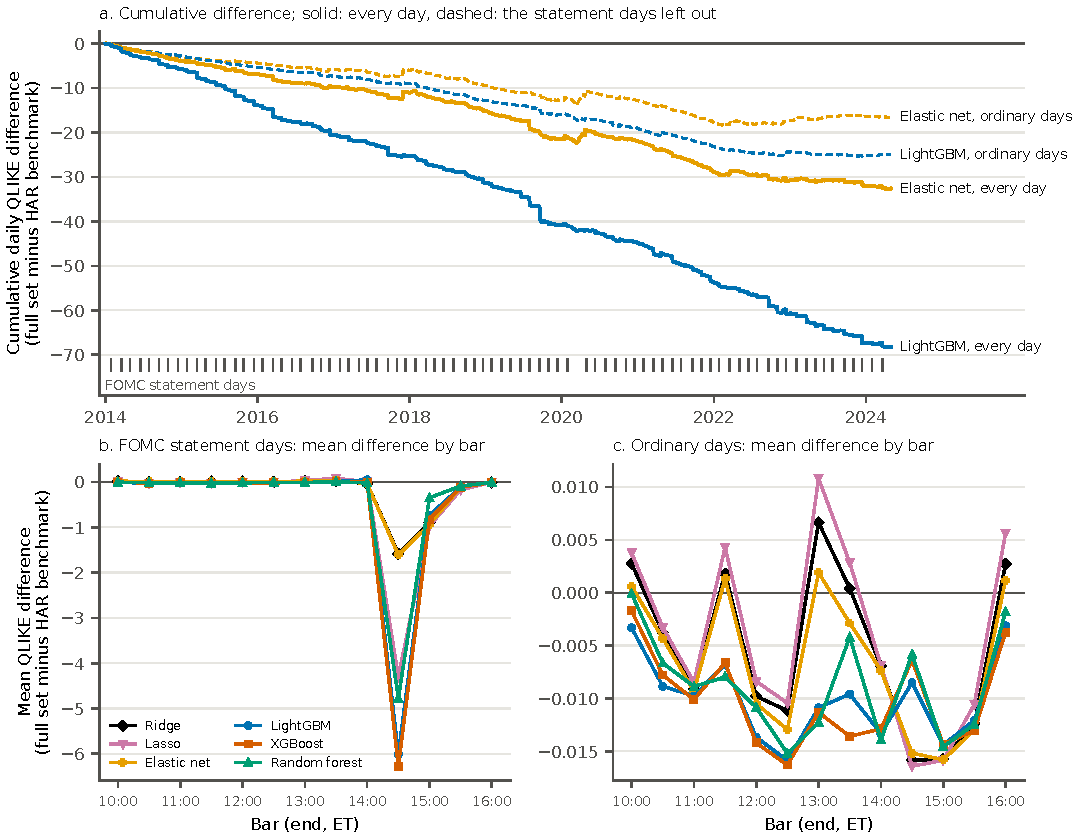
\includegraphics[width=\linewidth]{figures/rehaul_channels_cum.pdf}
\caption{Where the full set's gain over the HAR benchmark falls. (a) Cumulative sum through time of the daily QLIKE difference, full set minus HAR benchmark (the day's mean over its 13 bars; falling: the full set has the lower loss), for the elastic net and LightGBM; solid: every day; dashed: the same sum with the \rhchNEventDays{} scheduled FOMC statement days (ticks under the curves) left out. (b), (c) Mean difference by bar of the day (end stamps, ET) on the statement days and on the \rhchNOrdDays{} ordinary days, every class; note the different scales. Benchmarks as in Table~\ref{tab:rh_oos}; FOMC-patched design, \rhchNBars{} bars.}
\label{fig:rh_channels}
\end{figure}
